\documentclass	[11pt, a4paper, openany]{book} 
\usepackage[utf8]{inputenc}
\usepackage[francais]{babel}
\usepackage[T1]{fontenc}
\usepackage{amsmath}
\usepackage{amsfonts}
\usepackage{amssymb}
\usepackage{lmodern}
\usepackage{amsthm}
\usepackage{url}
\usepackage{graphicx} % ajout image
\usepackage[tt]{titlepic}%Centre le titre

\usepackage{shorttoc} %Permet d'avoir de petites tables des matières

\usepackage{eso-pic} %fond écran page de garde
\usepackage{shapepar} %texte en keur
\usepackage{siunitx} %S.I.

\usepackage{graphicx}
\usepackage{caption} %Permet d'ajouter des légendes en images sans les mettre en float + ds la marge
\usepackage{delarray} % Belles matrices

\usepackage{fancyhdr} %Permet de modifier l'entête & footer
\usepackage{bbding} % Note marge
\usepackage{todonotes}
\usepackage{wrapfig}

\pagestyle{headings} % Titre du ch et numéro page dans l'entete
\usepackage{fullpage} %Utilise toute la page

\usepackage{adjustbox}% empeche les box de sortir de la page

\newcommand{\theor}[1]{\adjustbox{minipage=\linewidth-2\fboxsep-2\fboxrule,fbox}{\textsc{Théorème : }#1}}

\newcommand{\lemme}[1]{\adjustbox{minipage=\linewidth-2\fboxsep-2\fboxrule,fbox}{\textsc{Lemme : }#1}}

\newcommand{\retenir}[1]{\adjustbox{minipage=\linewidth-2\fboxsep-2\fboxrule,fbox}{\textbf{\textit{\textsc{A retenir} : }}#1}}

\newcommand{\cst}{\text{cst}}
\newcommand{\E}{\vec E}
\newcommand{\F}{\vec F}

\newcommand{\corollaire}[1]{\ \\\begin{tabular}{|c}
\begin{minipage}{\textwidth}
  \textsc{Corollaire : } \textit{#1}
\end{minipage}
\end{tabular}}


\newcommand{\proposition}[1]{\adjustbox{minipage=\linewidth-2\fboxsep-2\fboxrule,fbox}{\textsc{Proposition : }#1}}


\newcommand{\questpm}[3]{#1. \textbf{#3} (p.#2)}
\newcommand{\exerc}[2]{\textbf{\Large Exercice #1\normalsize \\#2}}
\newcommand{\serie}{\sum_{k=1}^\infty}
\newcommand{\series}{\sum_{k=0}^\infty}
\newcommand{\dif}{\mathrm{d}}
\newcommand{\comment}[1]{}
\newcommand{\rot}{\text{rot}\,}
\newcommand{\divv}{\text{div}\,}
\newcommand{\phas}[1]{\underline{#1}}
\newcommand{\RE}{\text{Re}}
\DeclareMathOperator{\arccot}{arccot}
\newcommand{\com}[1]{}

%\newcommand{\oiint}{\int\!\!\!\!\!\:\!\!\!\;\!\!\subset\!\!\supset\!\!\!\:\!\!\!\!\!\int}
\newcommand{\oiint}{\int\!\!\!\!\!\!\! \:\!\subset\!\!\supset\!\!\!\!\!\!\!\int}
%%% Background %%%
\newcommand\BackgroundPic{%
\put(0,0){%
\parbox[b][\paperheight]{\paperwidth}{%
\vfill
\centering

\includegraphics[width=\paperwidth,height=\paperheight,%
keepaspectratio]{ulb.jpg}%
\vfill
}}}


\begin{document}
\renewcommand{\proofname}{Démonstration}
\frontmatter
%\mainmatter
\AddToShipoutPicture*{\BackgroundPic}
\begin{titlepage}
\begin{center}	
	
	\newcommand{\HRule}{\rule{\linewidth}{0.5mm}}   			%Titre en gros
	
\includegraphics[scale=0.11]{logo.jpg}~\\[1cm]				%Logo

	\textsc{\LARGE Université Libre de Bruxelles}\\[1.5cm]
	\textsc{\Large Synthèse}\\[0.5cm]

	\HRule \\[0.4cm]
	{ \huge \bfseries Analyse II \ \\MATH-H-200 \\[0.4cm] }


	\HRule \\[1.5cm]
		\begin{minipage}{0.4\textwidth}
		\begin{flushleft} \large
		
		\emph{Auteur :}\\
			Nicolas \textsc{Englebert}

			\end{flushleft}
			\end{minipage}
			\begin{minipage}{0.4\textwidth}
			\begin{flushright} \large
			%\emph{Tuteur :} \\		
			\end{flushright}
		\end{minipage}

	\vfill

% Bottom of the page
{\large Année 2014 - 2015}

\end{center}
\end{titlepage}
\chapter*{Appel à contribution}
\subsection*{Synthèse OpenSource}
\begin{wrapfigure}[5]{l}{4.5cm}
	
\includegraphics[scale=0.5]{git.png}
\end{wrapfigure}
Ce document est grandement inspiré de l’excellent cours donné 
par Marc Haelterman à l’EPB (École Polytechnique de Bruxelles), faculté de l’ULB (Université 
Libre de Bruxelles). Il est écrit par les auteurs susnommés avec l’aide de tous les autres étudiants 
et votre aide est la bienvenue ! En effet, il y a toujours moyen de l’améliorer surtout que si le 
cours change, la synthèse doit être changée en conséquence. On peut retrouver le code source à l’adresse 
suivante
\begin{center}
	\url{https://github.com/nenglebert/Syntheses}
\end{center}\ \\
Pour contribuer à cette synthèse, il vous suffira de créer un compte sur \textit{Github.com}. De
légères modifications (petites coquilles, orthographe, ...) peuvent directement être faites sur le
site ! Vous avez vu une petite faute ? Si oui, la corriger de cette façon ne prendra que quelques 
secondes, une bonne raison de le faire ! \\
\\
Pour de plus longues modifications, il est intéressant de disposer des fichiers : il vous 
faudra pour cela installer \LaTeX, mais aussi \textit{git}. Si cela pose problème, nous sommes 
évidemment ouverts à des contributeurs envoyant leur changement par mail ou n’importe quel autre 
moyen.\\
\\
Le lien donné ci-dessus contient aussi le \texttt{README} contient de plus amples informations, 
vous êtes invités à le lire si vous voulez faire avancer ce projet ! 

\subsection*{Licence Creative Commons}
\begin{wrapfigure}[3]{r}{2.8cm}
	
\includegraphics[scale=0.17]{CC}
\end{wrapfigure}
Le contenu de ce document est sous la licence Creative Commons : \textit{Attribution-NonCommercial-ShareAlike 
4.0 International (CC BY-NC-SA 4.0)}. Celle-ci vous autorise à l'exploiter pleinement, compte-
tenu de trois choses :
\begin{enumerate}
	\item \textit{Attribution} ; si vous utilisez/modifiez ce document vous devez signaler le(s) nom(s)
	      de(s) auteur(s).
	\item \textit{Non Commercial} ; interdiction de tirer un profit commercial de l’œuvre sans 
	      autorisation de l'auteur 
	\item \textit{Share alike} ;  partage de l’œuvre, avec obligation de rediffuser selon la même 
	      licence ou une licence similaire
\end{enumerate}
Si vous voulez en savoir plus sur cette licence :
\begin{center}
	\url{http://creativecommons.org/licenses/by-nc-sa/4.0/}
\end{center}

\begin{flushright}
	\textbf{Merci ! }
\end{flushright}
\tableofcontents



\mainmatter
%\part{Résumé du cours}

\setcounter{chapter}{14}
\chapter{Équations différentielles linéaires et systèmes différentiels linéaires}
\setcounter{section}{7}
\section{EDL à coefficients constants}
Rappelons la forme d'une EDL d'ordre $p$
\begin{equation}
\underbrace{a_0}_{\neq 0} y^{(p)} + a_1y^{(p-1)} + \dots + a_py = b
\end{equation}
Cette équation sera dite à coefficients constant si $\forall i : a_i =\ cste$. Si $b = 0$, l'équation sera dite homogène. Ne pas oublier le $y$ après le terme $a_p$ ! Reprenons le théorème démontré dans la section précédente (15.7)  :

\theor{L'ensemble des solutions de l'EDLH forme un espace vectoriel de dim p sur le corps $\mathbb{K}$}\ \\

Ce théorème a pour corollaire :\\
\corollaire{L'EDLH (régulière) possède $p$ solution linéairement indépendante $y_1, \dots, y_p$ et pour tout choix de telles solution, toute solution de l'EDLH en est combili (sur $\mathbb{K})$
$$S_0 = vect_{\mathbb{K}}\{y_1, \dots , y_p\}$$
$$S_0 = \{c_1y_1 + \dots + c_py_p ; c_i, \dots , c_p \in \mathbb{K}\}$$}
\ \\
L'ensemble des solutions (de l'EDLH) $y_1, \dots , y_p$ linéairement indépendant est appelé \textbf{système fondamental}  de solution de l'EDLH.\\

La forme d'une EDL d'ordre $p$ peut être notée sous une forme plus compacte :
\begin{equation}
Ly = b
\end{equation}
où $L$ est un opérateur différentiel linéaire tel que : 
\begin{equation}
L = P(D) = a_0D^p + \dots + a_{p-1} D + a_p D^0
\end{equation}
\subsection{Polynôme caractéristique et solutions exponentielles $e^{\lambda t}$}
Cherchons maintenant des solutions exponentielles de type $e^{\lambda t}$. Ceci est possible grâce à une \textit{formule magique}. Remarquons :
\begin{eqnarray}
D^1 e^{\lambda t} &=& \lambda e^{\lambda t}\\
D^2 e^{\lambda t} &=& \lambda^2 e^{\lambda t}\\
D^p e^{\lambda t} &=& \lambda^p e^{\lambda t}
\end{eqnarray}
Si $P(D)$ est l'expression ci-dessus alors :
\begin{equation}
P(D) e^{\lambda t} = P(\lambda)e^{\lambda t}
\end{equation}
On remarque que $P(\lambda)$ n'est rien d'autre que le polynôme caractéristique ! Si en plus les coefficients de l'équation sont constant, alors $e^{\lambda t}$ est dans $ker\ P(D) \Leftrightarrow \lambda$ est racine de $P$, c'est à dire si $y = e^{\lambda t}$ est solution de $P(D)y = 0$.\\
Plus mathématiquement, l'égalité ci-dessus montre que $e^{\lambda t}$ est solution de $P(D)y = 0 \Leftrightarrow P(\lambda) = 0$.\\ \textbf{Attention !} Il faut savoir démontrer que $P(D)$ est n opérateur linéaire pour l'examen.\\
On peut ré-écrire l'EDLH tel que:
\begin{equation}
EDL \equiv P(D)y = 0
\end{equation}
où $P$ est un polynôme de degré $p$ à coefficient constant.\\
Si le polynôme $P$ a $p$ racines distinctes $\lambda_1, \dots , \lambda_p$, alors on obtient $p$ solutions "exponentielles" $y_1(t) = e^{\lambda_1t}, \dots$ linéairement indépendantes. D'où la SG de l'EDL\textbf{H} : $y = c_1 y_1 + \dots + c_py_p$\\
Que faire dans le cas ou $\lambda$ est une racine double ? Il faut factoriser pour avoir:
\begin{equation}
D e^{\lambda t} = \lambda e^{\lambda t} \Leftrightarrow (D - \lambda)e^{\lambda t} = 0
\end{equation}
et ensuite appliquer le même résultat que précédemment.
\begin{center}
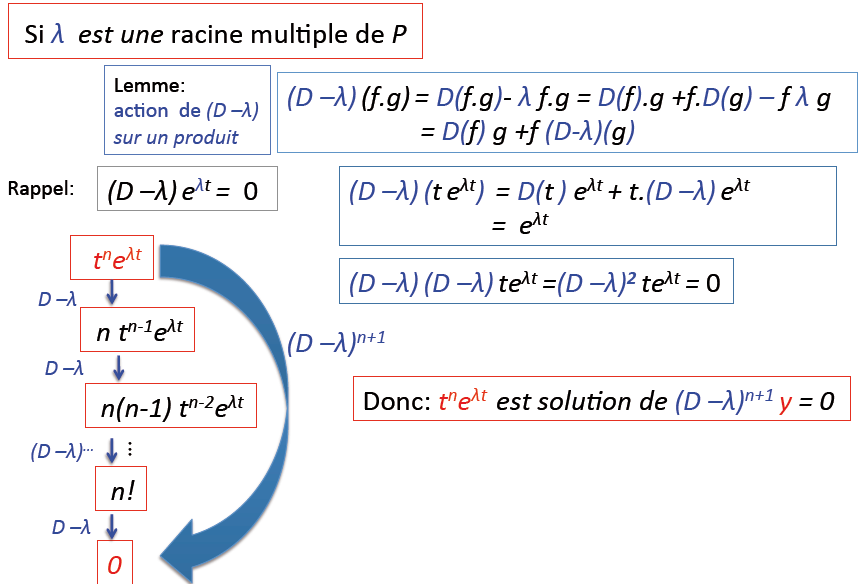
\includegraphics[scale=0.4]{image1.png}
\captionof{figure}{Cas des racines multiples}\footnote{Les solutions de \textbf{toutes} EDL\textbf{H}cc sont des combili d'exponentielles de polynômes $t^qe^{\lambda_j t}$}
\end{center}
Le polynôme en $D$ à coeff. constant, $P(D)$, peut être factoriser :
\begin{equation}
P(D) = (D - \lambda_1)\dots (D-\lambda_p)
\end{equation}
Est-ce aussi le cas de $P(D)$ l'opérateur linéaire ? Oui, car coeff $a_k$ sont constant !\\

Notons également que $D \lambda D = \lambda D^2$. Dès lors $P(D) \circ Q(D) = (P.Q)(D)$. \textbf{Par contre} $tD \circ D \neq D \circ tD$ !!

\subsection{Indépendance linéaire des exponentielles monômes}
Cette partie n'est pas à connaître.

\subsection{Méthodes des coefficients indéterminés}
Le but ici est de trouver une solution particulière à une équation de type :
\begin{equation}
P(D)y = a_0y^{(p)} + a_1 y^{(p-1)} + \dots + a_p y = g(x)
\end{equation}
Trois cas s'offrent à nous :
\subsubsection{1. Si $g(x)$ = polynôme de $deg\ m$}
On cherche une SP de type $y(x) = (c_0 x^n + \dots + c_m).x^s$ où $s$ est la multiplicité de 0 comme racine de $P(\lambda)$.\\
On procède ensuite comme dans le cours d'Analyse I (on dérive, on remplace, ...). \\
Pour savoir ce que vaut $s$, on peut regarder l'ordre de dérivation le plus petit, qui vaudra $s$.

\subsubsection{2. Si $g(x)$ = (polynôme de $deg\ m).e^{\alpha x}$}
On cherche une solution particulière de type $y = e^{\alpha x}(c_0 x^n + \dots + c_m).x^s$ où $s$ est la multiplicité de $\alpha$ comme racine de $P(\lambda)$.


\subsubsection{3. Si $g(x) = P_m(x).e^{\alpha x}.\sin / \cos (x)$}
On cherche une solution particulière de type $y = e^{\alpha x}\left(Q_m(x)\sin(\beta x) + R_m(x) \cos (\beta x)\right)x^s$ où $s$ est la multiplicité de $\alpha + i\beta$ comme racine de $P(\lambda)$.

\subsection{Stabilité asymptotique}
Une EDL dont la partie homogène EDLA n'a que des solutions asymptotiquement nulles est dite asymptotiquement stable.


\section{EDL équidimensionelle d'Euler}
Certaines équations différentielles ne sont pas à coefficients constant, mais on peu se ramener à cette forme en suivant cette méthode.\\
On ne s'est pas beaucoup attardé dessus, ce sera surement vu en séances de TP !

\textbf{Spoil :} elle a dit que généralement dans les examens précédents, il y a une équation à coefficient constant ou une équation d'Euler ! 

\setcounter{section}{6}
\section{Équation différentielles linéaires d'ordre $p$}
\subsection{Théorème général pour les EDL régulière}
Considérons l'EDL d'ordre $p$
\begin{equation}
\underbrace{a_0}_{\neq 0} y^{(p)} + a_1y^{(p-1)} + \dots + a_py = b
\end{equation}
où $a_i, b \in C^\circ(I, \mathbb{K})$ et $y \in C^p(I, \mathbb{K})$. Si $a_0$ ne s'annule pas sur $I$, l'EDL sera dite \textit{régulière}. Si ce n'est pas le cas, l'EDL est dite \textit{singulière} sur I : les zéros sont dits "points singuliers".
La forme "normale" d'une EDL régulière sur $I$ est :
\begin{equation}
y^{(p)} = -\frac{a_1}{a_n}y^{(y-1)} - \dots - \frac{a_p}{a_n}y + \frac{b}{a_n}
\end{equation}

Avant d'énoncer le fameux théorème, revenons sur une définition importante : un \textbf{système fondamental} de solution de $E_0$ est un ensemble de $p$ solutions de $E_0$ linéairement indépendantes.\\

\theor{\begin{enumerate}
\item L'ensemble des solution sur $I$ de l'EDLH est un espace vectoriel $S_0$ de dimension $p$ sur $\mathbb{K}$ (SEV de $C^p(I, \mathbb{K})$).

\item L'ensemble $S_b$\footnote{Sol. de l'EDLH} des fonctions solutions sur I de l'EDL est un translaté de $S_0$\footnote{Sol de l'EDLnH}. En bref : SGEnH = SPEnH + SGEH

\item Tout problème de Cauchy relatif à une EDL régulière sur $I$ possède une et une sole solution sur $I$, notée $t \mapsto y(t;t_0, (y_{0,0}, \dots , y_{0,p-1}), b)$
\end{enumerate}}\ \\
Comment démontrer le 1. ? Il faut commencer par démontrer que l'opérateur linéaire $L : C^p \rightarrow C^0 = y \mapsto L(y) := a_0y^{(p)} + \dots + a_p y$ est une application linéaire. Pour se faire, démontrons la propriété : $L(\lambda y + \mu x) = \lambda L(y) + \mu L(x)$.

\begin{proof}\ \\
$y \rightarrow y^{(k)}$ est linéaire car $\frac{d^k}{dt^k}(\lambda y + \mu x) = \lambda\frac{d^k y}{dt^k} + \mu \frac{d^kx}{dt^k}$.\\
$y \rightarrow a_ky^{(k)}$ est linéaire car : multiplication par une constante.\\
$Ly = \sum^k a_k y^k$ d'où : $a_k(\lambda y + \mu x)^k = \lambda a_k y^k + a_k \mu x^k$.\\
On peut sommer les A.L., donc $L$ est bien un opérateur linéaire.
\end{proof}

Ceci étant démontré, il faut maintenant démontrer que $S_0$ est de dimension $p$. Soit $t_0 \in I$ ("Evaluation de Cauchy" à l'instant $t_0$) et considérons l'application\footnote{Au vu de la C.I. de Cauchy (et du SDL associé à l'EDL) il est naturel d'associer la fonction vectorielle $\phi$} :
\begin{equation}
\phi = S-0 \rightarrow \mathbb{K}^p : y \mapsto \left( \begin{array}{c}
y(t_0)\\
y'(t_0) \\
\vdots \\
y^{(p-1)}(t_0)
\end{array} \right)
\end{equation}
$\phi$ applique l'espace vectoriel $S_0$ dans l'espace vectoriel $\mathbb{K}^p$ de dimension $p$.\\
Or, cette application est : 
\begin{enumerate}
\item linéaire (par la linéarité du problème de Cauchy)
\item surjective (Th. d'existence de la solution d'un problème de Cauchy)
\item injective (Th. d'unicité de la solution d'un problème de Cauchy)
\end{enumerate}
On peut donc dire que $\phi$ est un isomorphisme d'espace vectoriel, d'où : $dim\ S_0 = p$ sur $\mathbb{K}$.

\subsection{Wronskien et Jacobi-Liouville}
A tout ensemble de $p$ fonctions de classes $C^p$, on peut associer une fonction $W(y_1, \dots, y_p)$ et lui associer un "Wronskien" :
\begin{equation}
W(t, y_1,\dots,y_p) = \left|\begin{array}{l}
y_1(t)\ \ \   \ \ \  \  \dots  \  \ \  y_p(t)\\
\ \ \ \ \ \vdots\ \ \ \ \ \ \ \ \ \vdots\ \ \ \ \ \ \ \ \ \vdots\\
y_1^{(p-1)}(t)\ \ \dots\ \ \ y_p^{(p-1)}(t)
\end{array}\right|
\end{equation}
Voyons le théorème fondamental du Wronskien (EDLH d'ordre $p$ et régulière sur $I$): \\
\theor{\ \\$y_1,\dots,y_p$ sont linéairement indépendant\\
$\Leftrightarrow W(y_1,\dots, y_p)$ ne s'annule pas sur $I$\\
$\Leftrightarrow W(y_1,\dots, y_p)$ n'est pas identiquement nulle sur $I$}\ \\

On peut ainsi dire que $W$ s'annule quelque part $\Leftrightarrow W$ est nul partout.\\

Plus fort encore (si si!) on l'\textbf{équation de Jacobi-Liouville} décrit l'équation du wronskien à travers le temps:
\begin{equation}
W(t) = W(t_0)e^{-\int_{t_0}^t \frac{a_1}{a_0}}
\end{equation}
Comme l'exponentielle est toujours positive, $W(t)$ et $W(t_0)$ ont le même signe : l'un ne s'annule pas sans l'autre.

\begin{proof}\ \\
\begin{flalign*}
\text{Il faut prouver que $y_1,\dots,y_p$ sont linéairement dépendant} & \underset{(1)}{\Rightarrow} W(y_1,\dots,y_p) \text{ nul sur }I\\
 & \underset{(2)}{\Rightarrow} W(y_1,\dots,y_p) \text{ s'annule sur }I\\
 & \underset{(3)}{\Rightarrow} y_1,\dots,y_p \text{linéairement dépendant}\\
\end{flalign*}
$(1)$ Comme $y_1,\dots,y_p$ sont linéairement dépendant $\Rightarrow\exists \underbrace{c_1,\dots,c_p}_{\text{p scalaire}}\neq 0\,|\,c_1y_1+\dots+c_py_p=0$ (définition linéairement dépendant, 0 correspondant à la fonction nulle). Donc toutes les dérivées de cette fonction sont nulles, d'où
\begin{align*}
 & c_1y_1'+\dots+c_py_p' = 0\\
 & \vdots\\
 & c_1y^{(p-1)}_1+\dots+c_py^{(p-1)}_p = 0
\end{align*}
Donc, $\forall t\in I$, le système algébrique :$\left\{\begin{array}{l}
c_1(t)y_1(t)+\dots+c_p(t)y_p(t) = 0\\
\vdots\hspace{8cm}(*)\\
c_1(t)y^{(p-1)}_1(t)+\dots+c_p(t)y^{(p-1)}_p(t) = 0
\end{array}\right.$\\
possède 1 solution non triviale ($c_1(t),\dots,c_p(t)$). Donc le $\det = 0$ (qui est précisément le Wronskien $W(t;y_1,\dots,y_p)$)\\\\
$(2)$ Si $W(t;y_1,\dots,y_p)=0\,\forall t\Rightarrow W(t_0;y_1,\dots,y_p)=0, t_0\in I$\\\\
$(3)$ Si $W(t_0;y_1,\dots,y_p)=0\Rightarrow\exists (c_1,\dots,c_p),$ solution non triviale du système linéaire $(*)$ pour $t=t_0$. Considérons la fonction $\tilde{y} := c_1y_1+\dots+c_py_p$, solution de $(*)$ (combili de solution) et de plus, on peut dire que $\left\{\begin{array}{l}
\tilde{y}(t_0) := c_1y_1(t_0)+\dots+c_py_p(t_0)=0\\
\tilde{y}'(t_0) := c_1y_1'(t_0)+\dots+c_py_p'(t_0)=0\\
\vdots\\
\tilde{y}^{(p-1)}(t_0) := c_1y_1^{(p-1)}(t_0)+\dots+c_py_p^{(p-1)}(t_0)=0
\end{array}\right.$ Donc $\tilde{y}$ est solution au problème de Cauchy $\tilde{y}(t_0)=\tilde{y}'(t_0)=\dots=\tilde{y}^{(p-1)}(t_0)=0$ (pour $(*)$). Or la solution triviale satisfait le même problème, d'où $\tilde{y}=0$ par unicité de la solution. Ceci signifie donc que $y_1,\dots,y_p$ sont linéairement dépendant
\end{proof}


\subsection{Méthode de la variation des constantes}
Cette méthode - pour trouver une solution particulière - fonctionne toujours mais les calculs s'avèrent souvent plus longs.(Je suppose ça sera vu en TP!)\\
L'idée est la même que celle utilisée en BA1, il s'agit d'une généralisation : voici le slide associé :
\begin{center}
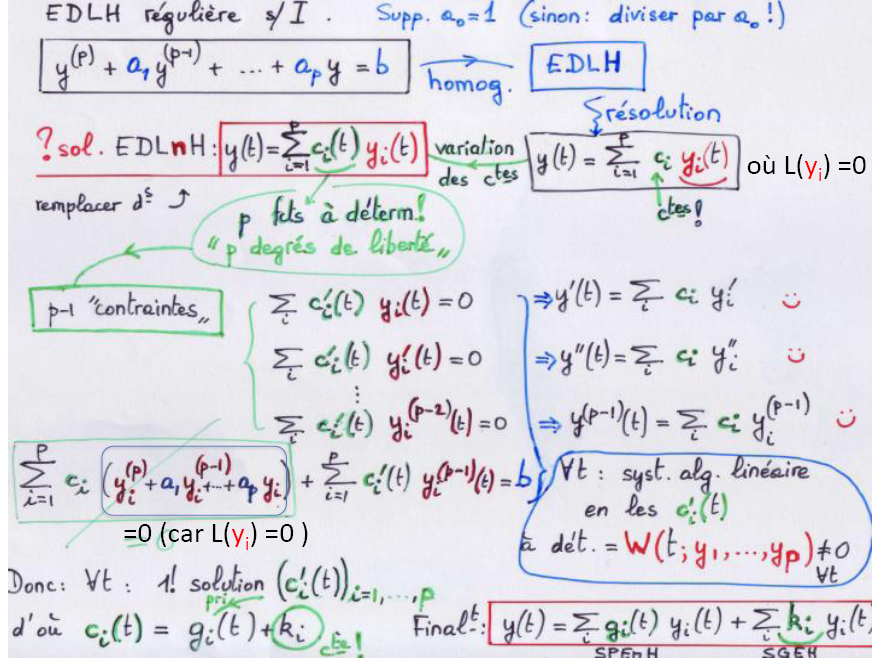
\includegraphics[scale=0.35]{image2.png}
\captionof{figure}{Justification de la méthode de la variation des constante}
\end{center}

\subsection{Fonction de Lagrange}
La j'avoue que je ne suivais plus trop, voici le slide associé..
\begin{center}
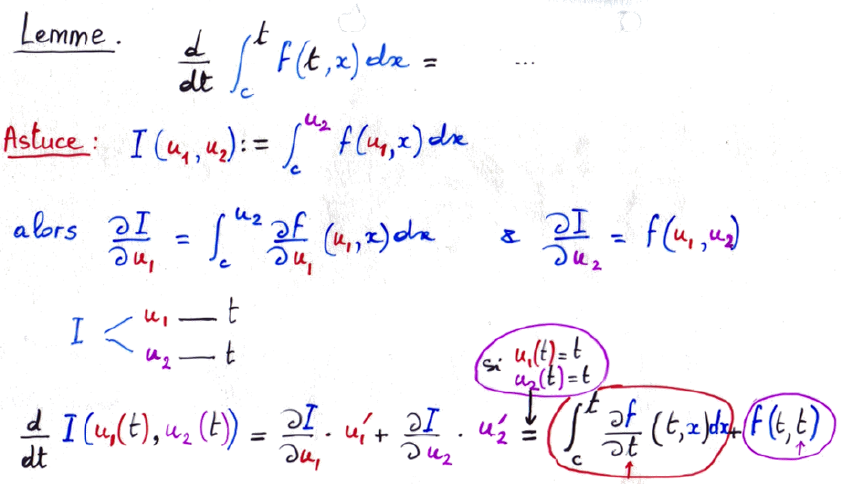
\includegraphics[scale=0.45]{image3.png}
\captionof{figure}{Fonction de Lagrange}
\end{center}
\begin{proof}\ \\
\begin{align*}
y'(t) & =\int_{t_0}^t\frac{\partial\ell}{\partial t}(t;\tau)f(\tau)\,d\tau+\ell(t;t)f(t)=\int_{t_0}^t\frac{\partial\ell}{\partial t}(t;\tau)f(\tau)\,d\tau\\
y''(t) & =\int_{t_0}^t\frac{\partial^2\ell}{\partial t^2}(t;\tau)f(\tau)\,d\tau+\frac{\partial\ell}{\partial t}(t;t)f(t)=\int_{t_0}^t\frac{\partial^2\ell}{\partial t^2}(t;\tau)f(\tau)\,d\tau\\
\vdots\\
y^{(p-1)}(t) &=\int_{t_0}^t\frac{\partial^{p-1}\ell}{\partial t^{p-1}}(t,\tau)f(\tau)\,d\tau+0\\
y^{(p)}(t) & =\int_{t_0}^t\frac{\partial^{p}\ell}{\partial t^{p}}(t,\tau)f(\tau)\,d\tau+\frac{\partial{p-1}\ell}{\partial t^{p-1}}(t,\tau)|_{\tau=t}f(\tau)|_{\tau=t}\\
 & =\int_{t_0}^t\frac{\partial^p\ell}{\partial t^p}(t,\tau)f(\tau)\,d\tau+\frac{f(t)}{a_0(t)}
\end{align*}
D'où le résultat (remplacer dans EDL, linéarité de $\int_{t_0}^t$ et la définition de $\ell(t,t_0)$)
\end{proof}
\iffalse
\subsection{Les opérateurs différentiels $D$ et $P(D)$}
Prochain cours ! 
Je teste l'ajout avec Dropbox
\fi 



\setcounter{section}{2}
\section{SDL à coefficients constants}
Soit 
\begin{equation}
Y' = AY + B
\end{equation}
où $A = (a_{ij})$ une matrice $m\times m$ indépendante de $t$.\\
$Y$ et $Y'$ sont des vecteurs colonnes tels que $Y = \left(\begin{array}{l}
y_1\\
\vdots\\
y_m
\end{array}\right)$ et $Y' = \left(\begin{array}{l}
y_1'\\
\vdots\\
y_m'
\end{array}\right)$
On connait les résultats pour $m=1$, on va tenter de généraliser. Ce sera facilement le cas si, par chance, la matrice $A$ est diagonalisable.

\subsection{Solutions exponentielles élémentaires du SDLHcc}
Si $m=1, SGENH \equiv y = ce^{At}$. Cherchons une solution particulière de la forme $Y = e^{\lambda t}V$ (tentons de généraliser le cas $m=1$) où $\lambda \in \mathbb{K}, V \in \mathbb{K}^m$.\\
Comme $\frac{d}{dt}(e^{\lambda t}V) = \lambda e^{\lambda t}V$ :\footnote{On remplace et on regarde la solution}
\begin{eqnarray}
Y &=& e^{\lambda t}V\ est\ solution\ de\ Y'=AY\\
&\Leftrightarrow & \lambda e^{\lambda t}V = Ae^{\lambda t}V\\
&\Leftrightarrow & \lambda V = AV\\
&\Leftrightarrow &V\ est\ vecteur\ propre\ de\ A\ de\ valeur\ propre\ \lambda
\end{eqnarray}
En effet, on sait que $AV = \lambda V \Leftrightarrow(A-\lambda I)V = 0$.\\
Géométriquement, le graphe de cette solution est une courbe (intégrale) plane de type exponentielle positive, constante ou exponentielle négative en fonction du signe de $\lambda$.\\
L'\textbf{orbite} de la solution (une \textbf{courbe} dans l'espace des phases) est incluse dans une droite passant par l'origine.

\subsection{Exemple}
Prenons un petit SDL tout gentil, tout mignon : $\left\{\begin{array}{l}
x' = x\\
y' = x-y
\end{array}\right.$. On peut le ré-écrire matriciellement comme :
\begin{equation}
\left(\begin{array}{l}
x\\
y
\end{array}\right)' = \left(\begin{array}{l}
1\ \ \  \ \ 0\\
1\ \ -1
\end{array}\right)\left(\begin{array}{l}
x\\
y
\end{array}\right)
\end{equation}
Il suffit de trouver les valeurs propres de $A$ (-1 et 1) ainsi que les vecteurs propres associés (flemme) et on trouve directement la solution en prenant une combili de $c_ie^{\lambda_i t}V_i$.

\subsection{Solution générale de $Y' = AY$ lorsque $A$ est diagonalisable}
\retenir{Si $V_1,\dots , V_m$ sont $m$ \textbf{vecteurs propres} de $A$ linéairement indépendants, de \textbf{valeurs propres} resp. $\lambda_1,\dots,\lambda_m$ sont $m$ \textit{solutions} de $Y' = AY$.\\
La solution générale de $Y' = AY$ est :
\begin{equation}
y(t) = \sum_{k=1}^m c_ke^{\lambda_k t}V_k
\end{equation}
On sait que si la matrice $A$ est diagonalisable, on n'aura pas besoin de chercher de "nouveaux" vecteurs propres, on en a suffisamment que pour écrire $m$ solutions linéairement indépendantes.}\ \\

Si l'on a une C.I. de Cauchy $y(0) = Y_0$ on peut écrire :
\begin{equation}
 \sum_{k=1}^m c_k e^0 V_k = Y_0
\end{equation}
On est dès lors ramené à un système dont la matrice est non-nulle car les vecteurs sont L.I $\rightarrow c_1, \dots,c_m$ sont univoquement déterminé et c'est d'ailleurs ce qui justifie l'unicité de la solution d'un problème de Cauchy !\\

Si la C.I. est plutôt $Y(t_0) = Y_0$, la solution n'est qu'un translaté :
\begin{equation}
 \sum_{k=1}^m c_k e^{\lambda_k(t-t_0)} V_k = Y_0
\end{equation}


\setcounter{subsection}{5}
\subsection{Exemples 2D lorsque A est diagonalisable}
\subsubsection{Deux valeurs propres de même signe}
\begin{wrapfigure}[7]{r}{4.5cm}
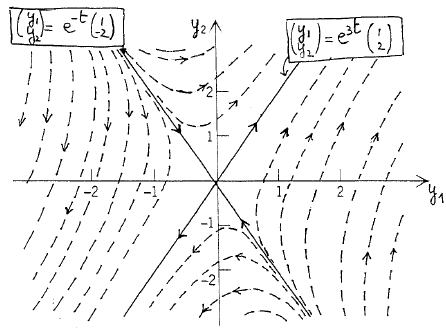
\includegraphics[scale=0.5]{image4.png}
\captionof{figure}{Valeurs propres de signe opposés}
\end{wrapfigure}
L'origine est un nœud.

\subsubsection{Deux valeurs propres de signe opposé}
L'origine est un point de selle.

\subsubsection{Cas de valeurs propres complexes non réelles}
Si $A$ est \textbf{réelle} et que $\vec y$ est une solution complexe de $\vec y' = A\vec y$ alors $Re\vec{y}\ et\ Im\vec{y}$ sont des solutions de ce système.\\ \

Si notre valeur propre est complexe, on peut écrire une solution complexe associée à ce groupe valeur propre/vecteur propre. On voit donc que à partir de la solution complexe, on peut en tirer deux solutions : une solution sera la partie réelle de cette solution et l'autre sera simplement la partie imaginaire.
\begin{center}
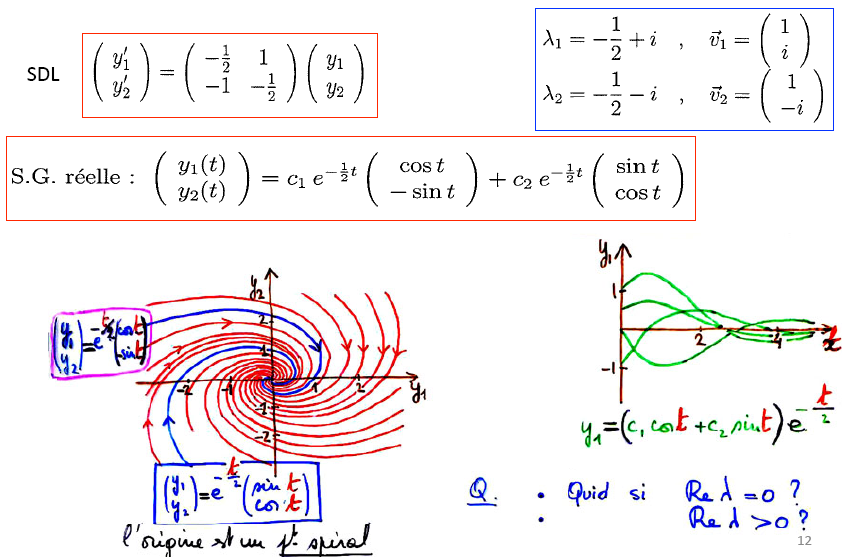
\includegraphics[scale=0.45]{image5.png}
\captionof{figure}{Valeurs propres complexes conjuguées - Exemple}
\end{center}
Si les deux valeurs propres sont conjuguées, l'origine est un point spiral. Ceci est logique du à la présence de sin et cos ainsi qu'à l'exponentielle positive/négative.


\setcounter{section}{1}
\section{Solution générale d'un SDL}
Avant tout, un $SDL$ régulier est est un SDL pouvant être mis sous cette forme :
\begin{equation}
Y'(t) = A(t)Y(t) + B(t)
\end{equation}
où les coeff $a_{ij}$ de $A$ sont des fonctions continues sur le connexe $I\subseteq \mathbb{R}$.\\
Un autre pré-requis important est le théorème d'existence et d'unicité :\\
\theor{Pour un tel $SDL$, tout problème de Cauchy (avec C.I. $Y(t_0) = 0$ où $t_0 \in I$) admet \textbf{une et une seule solution} $t \mapsto Y(t)$ sur $I$}
\subsection{L'espace vectoriel des solution d'un SDL$H$}
Soit le SDLH : $Y' = A(t)Y$. Soit $S$ l'ensemble des solutions de ce EDLH de I dans $\mathbb{K}^m$. La linéarité de ce SD nous indique directement qu'il s'agit d'un espace vectoriel sur $\mathbb{K}$.\\
Considérons l'application d'évaluation au temps $t_0$\footnote{Mes solutions sont des fonctions de $t$ et je l'évalue à $t_0$ : je regarde "ou on se trouve".}
\begin{equation}
\phi_{t_0} : S \rightarrow \mathbb{K}^m : Y \rightarrow Y/_{t_0}
\end{equation}
Cette application est :
\begin{itemize}
\item[Linéaire :] car $(\lambda Y + \mu Z)_{t_0} = \lambda Y_{t_0} + \mu Z_{t_0}$
\item[Bijective :] car $\forall Y_0 \in \mathbb{K}^m, \exists$ une seule solution (pb. de Cauchy)
\end{itemize}
Une application linéaire bijective est un isomorphisme : on peut en conclure que $dim\ S = m$.\\
\begin{center}
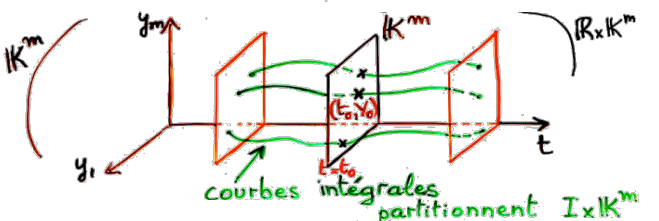
\includegraphics[scale=0.45]{image6.png}
\captionof{figure}{Courbes intégrales et problème de Cauchy}
\end{center}

Quand je prends un instantané je prends une section hyperplane et je regarde la valeur des courbes intégrales en celle-ci : si on fixe $t_0, y_0$, il passe une et une seule solution qui est une courbe intégrale.\\

\theor{L'ensemble des solution du SGH est un espace vectoriel de dimension $m$ et l'opérateur "évaluation des fonctions en $t=t_0$ est un isomorphisme d'espace vectoriel.}\ \\

\corollaire{Les $m$ solution $Y_1, \dots, Y_m$ sont linéairement indépendantes\\
 $\Leftrightarrow$ Les vecteurs $Y_1/_{t_0}, \dots, Y_m/_{t_0}$ sont linéairement indépendante (valable $\forall t$ fixé)}
 
\subsection{L'espace affin des solutions d'un SDLnH}
Pour faire simple, on peut dire que $SGSnH = SGSH +\ une\ SPSnH$. Il suffit de prendre une solution particulières (peut importe laquelle) et de l'additionner à la solution générale du système différentiel homogène.

\subsection{Système fondamental}
Un système \textbf{fondamental} de solutions du SDLH $Y'(t) = A(t)y(t)$ où $A \in M_m(\mathbb{K})$ est un ensemble de solution formant une base de l'espace $S$ des solutions, autrement dit c'est un ensemble de $m$ solutions linéairement indépendantes.\\
\textbf{Inclure slide 31  + la proposition}

\subsection{Wronskien et Jacobi-Liouville pour SDL}
\begin{eqnarray}
W' = (Trace\ A)W\\
W(t) = e^{\int_{t_0}^t (Trace\ A)}W(t_0)
\end{eqnarray}
Rappellons le beau corollaire :\\
\corollaire{Si $W(t)$ est nul une fois, il l'est $\forall t$. Réciproquement, s'il n'est pas nul pour un $t$, il ne sera jamais nul.}

\subsection{SHLnH : variation des constantes}
La démo n'est pas à connaître et ce résultat est plus de la matière du TP. La solution générale d'un système non-homogène sera :
\begin{equation}
Y(t) = \int_{t_0}^t M(t)(M^{-1}B)|_s + \underbrace{M(t)C}_{SGSH}
\end{equation}
où $M(t)$ est la matrice fondamentale $(y_1,\dots,y_m)$.

\setcounter{section}{0}
\section{ED, SD, courbes intégrales et orbites}
Clôturons ce chapitre par l'introduction (car plus "pédagogique")! 
\subsection{SD, champ de direction et courbes intégrales}
Une courbe intégrale du SD est le graphe de la solution du SD.

\subsection{Condition initiale (CI) (de Cauchy)}
Par le théorème d'existence et unicité du problème de Cauchy, on peut en déduire que deux courbes intégrales ne se coupent jamais.

\subsection{Orbites et espace des phases}
On dira que $(y_1(t), y_2(t)) :=$ la \textit{phase} à l'instant $t$ ou encore la \textit{position} dans le plan $oy_1y_2$.\\
La phase représente ainsi chacun des états successifs d'un phénomène en évolution. Si le mouvement est circulaires, notons que le graphe de $Y$ sera une hélice.

\subsection{SD autonomes}
On le sait maintenant, un système différentiel est :
\begin{equation}
Y'(t) = F(t, Y(t))
\end{equation}
Deux cas particuliers importants : 
\begin{enumerate}
\item $F$ indépendant de $t\ \ \Leftrightarrow : $ SD autonome
\item $F$ linéaire en $Y\ \ \ \ \ \ \ \Leftrightarrow : $ SDL
\end{enumerate}













\setcounter{chapter}{10}
\chapter{Séries numériques}
\section{Séries numériques : convergence et C.A.}
\subsection{Introduction}
Une séries est une somme contenant une infinité de termes. On appelle \textbf{série numérique} une expression du type :
\begin{equation}
a_1 + a_2 + a_3 + \dots = \sum_{k=1}^\infty a_k\ \ \ \ \ \ où\ \ \forall k : a_k \in \mathbb{C}
\end{equation}

\subsection{Suites arithmétiques et géométriques}
\subsubsection{Série arithmétique}
Une suite arithmétique est une suite $(s_k)_{k \geq 0}$ tel qu'il existe $a, a_0 \in \mathbb{C}$ tels que $s_k = ak + a_0\ \ \forall k \in \mathbb{N}_0$.\\
On lui associe facilement la série $a_0 + a + a + a + \dots = \sum_{k=0}^\infty a_k$ dont  le \textbf{terme général est constant} (ou presque) : $a_k = a$.
Cette série diverge ($+\infty$)

\subsubsection{Série géométrique}
On définit d'abord une suite $u_0 = u_0, u_1 = u_0\rho, u_2 = u_0\rho^2,\dots, u_3 = u_0\rho^k$. On peut lui associer la série $\sum_{k=0}^\infty u_0\rho^k$.\\
Si la raison ($\rho$) $\geq 0$, la série divergera si $\rho > 1$, convergera vers $u_0$ si $\rho = 1$ et vers $0$ si $\rho < 1$.

\subsubsection{Série harmoniques}
La première série (non trivialement divergente) dont on a montré rigoureusement la divergence est :
\begin{equation}
1 + \frac{1}{2} + \frac{1}{3} + \frac{1}{4} + \dots = \sum_{k=1}^\infty \frac{1}{k}
\end{equation}

\setcounter{subsection}{3}
\subsection{Convergence d'une série}
$\sum_{k=1}^\infty a_k$ \textbf{converge} ssi ($s_n$) converge.\\
La convergence de $s_n$ est donnée par $\forall \epsilon > 0 : \exists N : \forall n \geq N = |S_n - S| < \epsilon$.\\
Ou encore, $\sum_{k=1}^\infty a_k$ a pour \textbf{somme} $S$ ssi $s_n \rightarrow S$.

\setcounter{subsection}{5}
\subsection{Linéarite de la sommation des séries convergentes}
Attention, la réciproque ($\Leftarrow$) est fausse ! 
\begin{eqnarray}
\sum_{k=0}^\infty a_k\ converge\ &\Rightarrow & \sum_{k=0}^\infty \lambda a_k\\
\sum_{k=0}^\infty a_k\ et\ \sum_{k=0}^\infty b_k\ convergent \text{ (vers $A$ et $B$)} & \Rightarrow & \sum_{k=0}^\infty (a_k + b_k)\ converge\text{ (vers $A+B$)}
\end{eqnarray}

\subsection{Critère de Cauchy pour les séries}
Petit rappel du critère de Cauchy : $u_n$ est une suite de Cauchy $\Leftrightarrow$ :
\begin{equation}
\forall \varepsilon > 0, \exists N \in \mathbb{N}_0 : n,m \geq N \Rightarrow |u_n - u_m| < \varepsilon
\end{equation}
Le \textbf{critère de Cauchy} (pour les suites !) est : \\
\theor{Soit $(u_n)$ une suite de nombre réels. $(u_n)$ converge dans $\mathbb{R}$ ssi $(u_n)$ est une suite de Cauchy.}

\subsubsection{Critère de Cauchy pour les séries}
On dira que $\sum_{k=1}^\infty a_k$ converge $\Leftrightarrow$
\begin{equation}
\forall \epsilon > 0 : \exists K > 0 : \forall k \geq K, \forall h \geq 1 : |s_{k+h} - s_k| < \epsilon
\end{equation}

\subsection{Évanescence du terme général}
Une proposition nécessaire mais \textbf{non suffisante} importante est la suivante : \\

\proposition{Une condition nécessaire pour que la série $\sum_{k=1}^\infty a_k$ converge est que la suite $(a_k)_{k\geq 1}$ tende vers 0.}\ \\

Cette proposition est très utilisée sous sa forme contra posée :
\begin{equation}
a_k \nrightarrow 0 \Rightarrow \sum_{k=1}^\infty a_k\ \ \ diverge
\end{equation}
\begin{proof}\ \\
Nous avions que $|s_{k+h} - s_k| < \varepsilon$, ce qui peut aussi s'écrire $$\left|\sum_{n=k+1}^{k+h}a_n\right| < \varepsilon\Leftrightarrow\forall\varepsilon>0,\exists K>0:\forall m\geq k\geq K : \left|\sum_{i=k}^ma_i\right|<\varepsilon$$ et donc en particulier si $k=m$, on a $$|a_k|<\varepsilon$$
\end{proof}
\subsection{Convergence absolue}
Une nouvelle définition spécifique aux séries est nécessaire. On dira que la série $a_k$ \textbf{converge absolument}$\Leftrightarrow$ cette même série en valeur absolue converge. Cette définition nous amène à la proposition :

\proposition{Une condition suffisante pour que $\sum_{k=1}^\infty a_k$ converge est que $\sum_{k=1}^\infty a_k$ converge absolument}\ \\

Ce qui peut se résumer à : convergence absolue $\Rightarrow$ convergence\footnote{La réciproque est fausse : considérer la "série harmonique alternée" : $\sum_{k=1}^\infty a_k \frac{(1-)^k}{k}$}. $$\sum_1^{\infty}|a_k|\ conv\Rightarrow \sum_1^{\infty}a_k\ conv$$
\begin{proof}
\ \\
Il faut traduire la convergence dans le langage de Cauchy (Application du critère de Cauchy) et y appliquer l'inégalité triangulaire : $\sum_{k=1}^\infty |a_k|$ converge :
\begin{eqnarray}
&\Leftrightarrow & \forall \epsilon > 0, \exists K > 0 : \forall k \geq K, \forall l \geq 1 : \left|\sum_{i=k}^{k+l} |a_i| \right| < \epsilon\\
&\Rightarrow & forall \epsilon > 0, \exists K > 0 : \forall k \geq K, \forall l \geq 1 : \left|\sum_{i=k}^{k+l} a_i \right| < \epsilon\\
&\Leftrightarrow & \sum_{k=1}^\infty a_k\ \ \text{converge}
\end{eqnarray}
\end{proof}


\subsection{Séries à termes positifs}
Une série à termes positifs (= si le premier terme est positif) est définie :
\begin{equation}
\sum_{k=1}^\infty a_k\ \ \ \ \ \ où\ \ \ \ \forall k : a_k \geq 0
\end{equation}
Cette série étant croissante par propriété, elle ne convergera que si elle est majorée $ssi$ : 
\begin{equation}
\exists M \in \mathbb{R} : \forall n \in N \sum_{k=1}^\infty a_k\ \leq M
\end{equation}  On peut conclure que une série à termes positifs croissante converge $ssi \sum_{k=1}^\infty a_k\ < \infty$.

\section{Critères comparatifs}
Introduisons d'abord les intégrales généralisées. Si $f$ est positive ou nulle, bornée et intégrale alors l'intégrale généralisable à pour définition :
\begin{equation}
\int_0^\infty f := \lim\limits_{r \rightarrow +\infty}  \int_1^r f
\end{equation}
Si $f \geq 0$ alors $\lim\limits_{r \rightarrow \infty}  \int_1^r f$ existe dans $\mathbb{R} \Leftrightarrow$ l'ensemble $\{\int_1^r f\}$ est borné supérieurement dans $\mathbb{R}$. Dit de façon plus sympathique :
\begin{equation}
\lim\limits_{r \rightarrow \infty} f < \infty
\end{equation}
\subsection{Critère intégral de Cauchy}
Le \textbf{critère intégral de Cauchy} s'énonce :\\

\proposition{Si $f$ est positive, décroissante et intégrable sur tout compact $\subset \mathbb{R}^+_0$, alors
\begin{center}
  $\sum_{k=1}^\infty f(k)$ converge $ssi\ \int_1^\infty f(x)\ \text{dx}$ converge.
 \end{center}}
 
\begin{proof}
\ \\
Soit $f$ une fonction tel que $\forall k \in \mathbb{N}_0 : f(k) = a_k$. Comme la fonction décroit, je peux  écrire :
\begin{equation}
f(k) \geq f|_{[k, k+1]} \geq f(k+1)
\end{equation}
En passant à l'intégrale sur chaque membre (Sur les deux termes extrêmes $f(k)$ est constant et l'intégrale donne juste $k+1-k = 1$) :
\begin{equation}
f(k) \geq \int_k^{k+1} f \geq f(k+1)
\end{equation}
En multipliant par $\sum_k$ :
\begin{equation}
\sum_{k=1}^n f(k) \geq \int_1^{n+1} f \geq \sum_{k=1}^n \underbrace{f(k+1)}_{a_{k+1}}
\end{equation}
D'où on tire, par def. de $a_k$ :
\begin{equation}
\sum_{k=1}^n a_k \geq \int_n^{n+1} f(x)\ dx \geq \sum_{k=2}^{n+1} a_k
\end{equation}
\end{proof}

\setcounter{subsection}{4}
\subsection{Série de Riemann}
\proposition{\begin{equation}
\sum_{k=1}^\infty \frac{1}{k^\alpha}\ \text{converge}\ ssi\ \alpha > 1
\end{equation}}
\begin{proof}\ \\
\begin{itemize}
\item Si $\alpha \leq 0$, le terme général ne tend pas vers 0, d'où la divergence de la série.
\item Si $\alpha > 0$, on peut utiliser le critère intégral de Cauchy. La fonction $x \rightarrow \frac{1}{x^\alpha}$  est positive et décroissante et l'intégrale généralisée $\int_1^\infty \frac{1}{x^\alpha}dx$ converge $ssi\ \alpha > 1$ d'où le résultat annoncé.
\end{itemize}
\end{proof}
\begin{center}
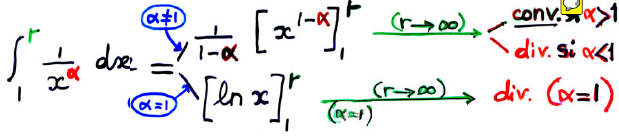
\includegraphics[scale=0.7]{image7.png}
\captionof{figure}{Série de Riemann}
\end{center}

\subsection{Critère de comparaison}
\theor{S'il existe $K$ tel que $\forall k \geq K : |a_k| \leq b_k$, alors la convergence de $\sum_{k=1}^\infty b_k$ entraîne la convergence absolue de $ \serie a_k$.\\
Autre version, plus mathématique :
\begin{equation}
\left.\begin{array}{l}
\forall k : |a_k| \leq M_k\\
\serie M_k\ \ \text{converve}
\end{array}\right\}\ \Rightarrow \serie a_k\ \ \text{C.A.}
\end{equation}}\ \\
\begin{proof}
\ \\
Par hypothèse $\serie b_k$ converge. Il en résulte directement de l'hypothèse que :
\begin{equation}
\exists M \in \mathbb{R}, \forall n : \sum_{k=1}^n b_k < M
\end{equation}
Ceci étant supérieure à l'expression suivante :
\begin{equation}
\exists M \in \mathbb{R}, \forall n : \sum_{k=1}^n |a_k| < M
\end{equation}
Il en résulte que cette dernière est croissante et majorée dans $\mathbb{R}$, donc convergente.
\end{proof}

\subsection{Critère d'équivalence}
\proposition{Supposons qu'il $\exists K : \forall k \geq K : a_k \geq 0, b_k > 0$ et que la limite suivant existe au sens large : $\lim\limits_{k \rightarrow \infty} \dfrac{a_k}{b_k} =: l \in \overline{\mathbb{R}^+}$.\\
Distinguons les cas suivants :
\begin{enumerate}
\item Si $0 < l < +\infty$ : $\serie a_k\ \text{converge} \Leftrightarrow\ \serie b_k\ \text{converge}$
\item Si $l = 0:\ \ \ \ \ \ \ \ \Leftarrow$
\item Si $l = +\infty :\ \ \ \ \ \Rightarrow$
\end{enumerate}}\ \\
Le sens de l'implication est logique, car (par exemple) pour le cas $l=0$ cela signifie que $b_k$ grandit plus vite que $a_k$, d'où le $\Leftarrow$.

\section{Critères absolus}
\subsection{Critères du quotient}
La critère du quotient s'exprime (en couleur, ça faisait longtemps) :
\begin{center}
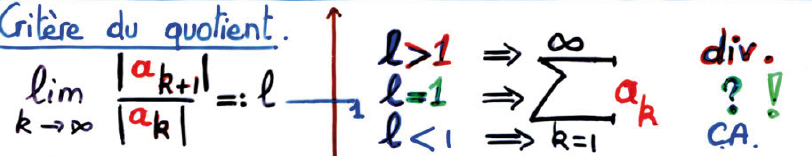
\includegraphics[scale=0.55]{image8.png}
\captionof{figure}{Critère du quotient}
\end{center}
Le cas de $l = 1$ ne donne aucune information. Dans l'exemple suivant, le quotient $l$ vaut chaque fois l'unité :
\begin{equation}
\left\{\begin{array}{l}
\serie \dfrac{1}{k}\ \text{diverge}\ \ \ \ \ mais\ \lim\limits_{k \rightarrow \infty} \dfrac{\frac{1}{k+1}}{\frac{1}{k}} = 1\\
\serie \dfrac{1}{k^2}\ \text{converge}\ \ \ mais\ \lim\limits_{k \rightarrow \infty} \dfrac{(\frac{1}{k+1})^2}{\frac{1}{k^2}} = 1
\end{array}\right.
\end{equation}

\setcounter{subsection}{2}
\subsection{Critère de la racine}
\proposition{Si $\lim\limits_{k \rightarrow \infty} \sqrt[k]{|a_k|} = r$ (si la limite existe et vaut $r$), alors :
\begin{enumerate}
\item Si $r < 1$ alors $\serie a_k$ converge absolument
\item Si $r = 1$ alors $\serie a_k$ peut converger ou diverger
\item Si $r > 1$ alors $\serie a_k$ diverge
\end{enumerate}}\ \\
\begin{proof}\ \\
1. $r<1\rightarrow r+\varepsilon<1$ et $\sqrt[k]{|a_k|}\leq r+\varepsilon\Rightarrow |a_k|\leq(r+\varepsilon)^k$ et par le critère de comparaison  $\sum_1^{\infty}(r+\varepsilon)^k\ conv$ car $(r+\varepsilon)<1$ et donc $$\Rightarrow\sum_1^{\infty}|a_k|\ conv\Rightarrow\sum_1^{\infty}a_k\ C.A.$$\ \\
2. Par Riemman\\\\
3. $l>1\rightarrow\sqrt[k]{|a_k|}>1\Rightarrow|a_k|>1$ La CN de convergence ($a_k\rightarrow0$) n'est donc pas respectée, la série diverge
\end{proof}
\section{Séries alternées et généralisation}
\subsection{Critère des séries alternées}
Une série $\serie a_k$ est dite \textbf{alternée} si son terme général alterne de signe. Toute série alternée peut donc se mettre sous la forme $\serie (-1)^kb_k$ ou $\sum_{k=0}^{\infty} (-1)^kb_k$\\

\proposition{Si la suite $b_k$ est décroissante et tend vers 0, alors $\serie (-1)^kb_k$ converge.}\ \\

L'implication est bien $b_k$ décroissant $\Rightarrow$ la convergence mais la réciproque est fausse ($\nLeftarrow$) !

\subsection{Démonstration du critère}
\begin{proof}\ \\
Soit la somme partielle $s_n=\sum_{k=0}^n(-1)^kb_k$, décomposons la en termes pairs et impairs : $s_{2n+1}$ et $s_{2n}$. Comme les termes $b_k$ décroissent, on peut dire :\begin{enumerate}
\item $s_{2n+2}-s_{2n}=b_{2n+2}-b_{2n+1}\leq0$, on voit donc que la suite $(s_{2n})$ est décroissante, donc : $$s_{2n}=\underbrace{(b_0-b_1)}_{\geq0}+\underbrace{\dots}_{\geq0}+b_{2n}\geq0$$ Elle est donc décroissante et minorée, impliquant sa convergence vers $s_2$
\item $s_{2n+3}-s_{2n+1} = b_{2n+2}-b_{2n+3}\geq0$, on voit donc que la suite $(s_{2n+1})$ est croissante, donc : 
$$ s_{2n+1} = b_0-\underbrace{(b_1-b_2)}_{\geq0}-\dots-\underbrace{(b_{2n-1}-b_{2n})}_{\geq0}-b_{2n+1}\leq b_0$$ Elle est donc croissante et majorée, impliquant sa convergence vers $s_1$
\item $s_1$ et $s_2$ coïncident car : $s_2-s_1=\lim\limits_{n\rightarrow\infty}s_{2n}-\lim\limits_{n\rightarrow\infty}s_{2n+1} = \lim\limits_{n\rightarrow\infty}(s_{2n}-s_{2n+1})=\lim\limits_{n\rightarrow\infty}b_{2n+1}=0$ (puisque par hypothèse, $b_k\rightarrow0$)
\end{enumerate}
\end{proof}

\subsection{Erreur de troncature pour les séries alternées amorties}
\begin{equation}
\left| \serie (-1)^kb_k - \sum_{k=0}^n (-1)^kb_k \right| = |s - s_n| \leq b_{n+1}
\end{equation}
Cela signifie que la valeur absolue de l'erreur de troncature d'une série alternée amortie est majorée par la valeur absolue du premier terme.
\begin{proof}\ \\
Comme $(s_{2n})\searrow s\ \ (0\leq s_{2n}-s\Rightarrow s\leq s_{2n})$ et $(s_{2n+1})\nearrow s\ \ (-s\leq -s_{2n+1}\Rightarrow s-s{2n+1}\geq0)$, on peut dire que :$$\left\{\begin{array}{l}
0\leq s_{2n}-s\leq s_{2n}-s_{2n+1}=b_{2n+1} \\
0\leq s-s_{2n+1}\leq s_{2n+2}-s_{2n+1} = b_{2n+2}
\end{array}\right.\Rightarrow |s-s_n|\leq b_{n+1}$$
\end{proof}
\setcounter{subsection}{5}
\subsection{Critère d'Abel}
Le critère d'Abel nous informe que si $b_k$ tend vers zéro et que l'ensemble des sommes partielles est bonré ($|\sum_{k=0}^n \epsilon_k | \leq M$) alors la série $\serie \epsilon_kb_k$ converge.
\begin{equation}
\left.\begin{array}{l}
a_k \searrow0\\
|\serie \epsilon_k| \leq M
\end{array}\right\}\ \Rightarrow \serie (\epsilon_k a_k)\ \ \text{converge}
\end{equation}
C'est une condition suffisante, mais non nécessaire. Ce critère est particulièrement utile dans l'étude de la convergence des séries "amorties", c'est-à-dire dont la valeur absolue du terme général tend vers zéro en décroissant.

\section{Regroupement et permutation de termes}
\subsection{Regroupement de termes}
Petite propriété sympa (bien qu'un peu simple) ! Elle dit que si $\serie a_k$ \textbf{converge}, l'introduction de parenthèses ne change rien à la convergence de la série.


\subsection{Permutation de termes d'une série à terme $\geq 0$}
On ne modifie ni la convergence ni la somme d'une série à termes positifs en modifiant l'ordre de ses termes.\\
Si $\pi$ est une permutation dans $\mathbb{N}_0$ alors :
\begin{equation}
\serie a_k = S \Rightarrow \serie a_{\pi(k)} = S
\end{equation}

\begin{proof} (pas a connaitre)\\
Il suffit de montrer que le suprémum d'une série vaut celui de l'autre. Posons $M_n = \text{max}\{\pi(1), \dots, \pi(n)\}$ alors $\forall n$ :
\begin{equation}
a_{\pi(1)} + \dots + a_{\pi(n)} \leq a_1 + a_2 + \dots + a_{M_n} \leq \text{sup}_n \sum_{k=1}^n a_k
\end{equation}
On en tire que le le suprémum de la série permutée est inférieur au suprémum de la série initiale.\\
En faisant pareil raisonnement avec le minimum, on retrouve l'inverse.
\end{proof}

\subsection{Parties positive et négative d'une série}
\begin{wrapfigure}[10]{r}{4.5cm}
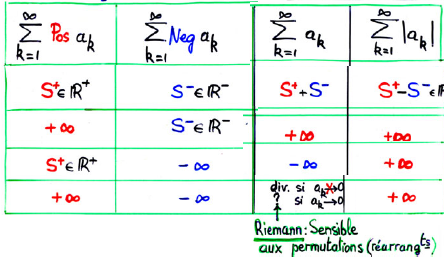
\includegraphics[scale=0.5]{image9.png}
\captionof{figure}{Semi-convergence en fonction de $a$}
\end{wrapfigure}
Imaginons une série donnant lieu à des termes parfois positifs et d'autres fois négatifs. Définissons les parties positives et négatives d'une réel $a$ de la sorte :
\begin{equation}
\text{Pos }a := \left\{\begin{array}{l}
a\ si\ a \geq 0\\
0\ si\ a <0
\end{array}\right. \ \ \ \ \ \ \text{Neg }a := \left\{\begin{array}{l}
0\ si\ a \geq 0\\
a\ si\ a <0
\end{array}\right. \ \
\end{equation}
On a ainsi $a =$ Pos $a$ + Neg $a$ et $|a| =$ Pos $a$ - Neg $a$.\\
Le tableau ci-contre reprend la semi-convergence (car pas de C.A.) de $\serie a_k$.


\setcounter{subsection}{4}
\subsection{Désordre chaotique de la semi-convergence}
\proposition{Soit $\sigma \in \vec{\mathbb{R}}$. Si $\serie a_k$ est une série réelle semi-convergente, alors il existe une permutation $\pi$ de $\mathbb{N}_0$ telle que $\serie a_{\pi(k)} = \sigma$.}\ \\

On en conclut que si une série converge absolument, on peut permuter les termes sans risque. Par contre, en cas de semi-convergence (converge mais pas absolument) la "sous-série positive" (et négative) ne sont pas bornées : On peut arranger les termes pour obtenir n'importe quoi !!!


\section{Produits de deux séries}
\subsection{Que faire ?}
Soient $\serie a_k$ et $\serie b_k$. Par analogie, on aurait envie de dire que leur produit donne :
\begin{equation}
\sum_{(k,l) \in \mathbb{N}\times\mathbb{N}} a_kb_l
\end{equation}
Mais il ne faut pas oublier que l'ordre des termes peut avoir une importance! Ce sera sans importance si tous les termes sont positifs ou en cas de convergence absolue mais pas en cas de semi-convergence.

\subsection{Le produit de deux séries absolument convergentes}
\theor{Si les séries $\serie a_k$ et $\serie b_l$ convergent absolument, alors $\sum_{(k,l) \in \mathbb{N}\times\mathbb{N}} a_kb_l$ converge absolument quel que soit l'ordre de sommation.}\ \\
La démonstration n'est pas à connaître, on peut "admettre" ce résultat dans le cadre de ce cours.

\newpage
\subsection{Le produit de Cauchy}
\begin{wrapfigure}[10]{l}{3.5cm}
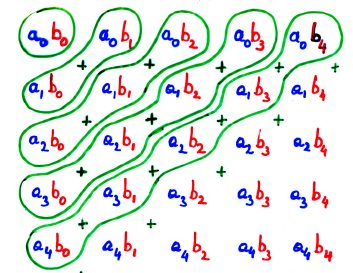
\includegraphics[scale=0.3]{image10.png}
\captionof{figure}{Produit de Cauchy}
\end{wrapfigure}
Pour dénombrer $\mathbb{N}\times\mathbb{N}$ il est naturel de choisir l'ordre de succession des couples $(k,l)$ proposée dans la figure ci-contre.\\

Par \textbf{définition}\footnote{Le slide 46 et la page 50 donne la motivation de cette définition.}, le \textit{produit de Cauchy} des séries $\serie a_k$ et $\serie b_k$ est la série :
\begin{equation}
\serie\left(\sum_{j=0}^k a_j b_{k-j}\right)
\end{equation}

\subsection{De la convergence du produit de Cauchy}
Le produit de Cauchy de deux série ne converge pas nécessairement même si les deux séries initiales l'étaient toutes deux.\\

Heureusement, nous savons que si deux séries convergent absolument, alors leur produit de Cauchy converge. Le théorème suivant (\textbf{Cauchy-Mertens}), que nous admettrons, généralise ce fait :\\

\theor{Si les deux séries $\serie a_k$ et $\serie b_k$ convergent et que l'une d'entre elles converge absolument, alors leur produit de Cauchy converge.}

\section{Séries complexes, séries vectorielles}
\begin{center}
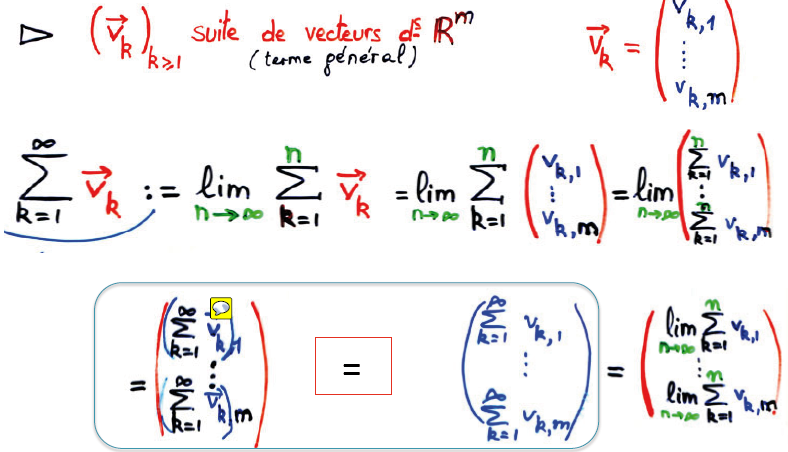
\includegraphics[scale=0.55]{image11.png}
\captionof{figure}{Série vectorielle}
\end{center}
Ce slide montre que la convergence d'une série de vecteurs peut se calculer composante par composante.\\
En 2D, on peut dire que :
\begin{equation}
\serie \left(\begin{array}{l}
x_k\\
y_k
\end{array}\right) = \left(\begin{array}{l}
X\\
Y
\end{array}\right)\ \ \ \ \Leftrightarrow\ \ \ \ \left\{\begin{array}{l}
\serie x_k = X\\
\serie y_k = K
\end{array}\right.
\end{equation}
Considérons maintenant le cas de la série complexe : $\serie z_k$ où $z_k \in \mathbb{C}$.\\
Toujours en 2D, on peut dire que :
\begin{equation}
\serie (x_k + iy_k) = X + iY\ \ \ \ \Leftrightarrow\ \ \ \ \serie \left(\begin{array}{l}
x_k\\
y_k
\end{array}\right) = \left(\begin{array}{l}
X\\
Y
\end{array}\right)\ \ \ \ \Leftrightarrow\ \ \ \ \left\{\begin{array}{l}
\serie x_k = X\\
\serie y_k = K
\end{array}\right.
\end{equation}
On peut ainsi décomposer une série complexe en séries réelles.\footnote{Re($\serie z_k$) : $\serie Re(z_k)$}

\subsection{Critère de Cauchy et CN de convergence}
Si $||\vec{v_k}|| \nrightarrow 0\ \ \Rightarrow \serie v_k$ diverge.

\subsection{Convergence absolue}
\proposition{$\serie \vec{v_k}$ C.A. $\Leftrightarrow\ \serie ||\vec{v_k}||$ converge.}\ \\
La convergence absolue implique (par Cauchy) que $\serie\vec{v_k}$ converge, mais la réciproque est fausse (la convergence absolue est une notion plus forte). Rappelons le nous avec notre contre-exemple fétiche :
\begin{equation}
\serie \frac{(-1)^k}{k}
\end{equation}
Cette série converge, mais ne converge pas absolument.

\section{Séries de puissances entières et positives}
\subsection{Séries de Taylor}
La \textbf{série de Taylor} de $f$ autour de $x_0$ en $x\in I$ est :
\begin{equation}
T_{f,x_0,\infty}(x) := \series \frac{f^{(k)}(x_0)}{k'}(x-x_0)^k\ \ \ \ \ f \in C^\infty
\end{equation}
On s'occupera plus tard de la bonne convergence de la série vers la "bonne somme (c'est à dire $f(x)$. Mais pour le moment, généralisons les séries  de Taylor en écrivant :
\begin{equation}
\series c_k(x-x_0)^k
\end{equation}
Il s'agit d'une \textbf{série de puissances (entière et positives)} définie $\forall x \in \mathbb{C}$.\footnote{Plus facile de travailler dans $\mathbb{C}$ dans ce cas!}

\subsection{Domaine de convergence d'une série entière dans $\mathbb{C}$}
Cherchons le \textit{domaine de convergence}, c'est à dire l'ensemble des $z$ pour lesquels la série numérique complexe
\begin{equation}
\series c_k(z-z_0)^k
\end{equation}
converge.
En utilisant le \textit{critère du quotient} et le \textit{critère de la racine}\footnote{Page 57-58.} :
\begin{center}
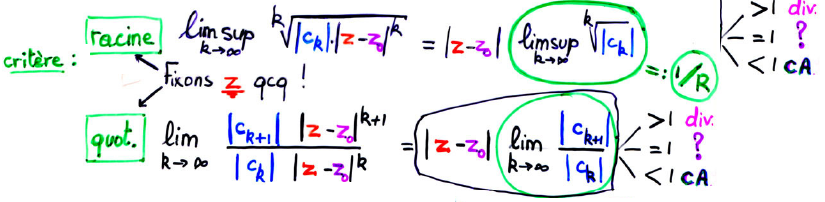
\includegraphics[scale=0.55]{image12.png}
\captionof{figure}{Domaine de convergence d'une série entière}
\end{center}
\theor{On trouve alors le \textbf{Théorème de Cauchy-Hadamard} stipulant que la série :
\begin{itemize}
\item \textit{Diverge} si $|z-z_0| > R$
\item \textit{C.A.} si $|z-z_0| < R$
\item \textit{Indet.} si $|z-z_0| = R$
\end{itemize}
où $R = \text{lim sup} \dfrac{1}{\sqrt[k]{|c_k|}}$.}

\subsection{Convergence au bord du domaine}
\begin{wrapfigure}[10]{r}{3cm}
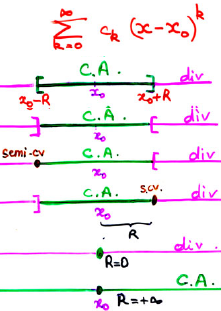
\includegraphics[scale=0.5]{image13.png}
\captionof{figure}{Six possibilités réelles}
\end{wrapfigure}
Les deux théorèmes (racines et quotient) ne savent rien nous dire sur la convergence au bord du domaine (au bord du disque de convergence, c'est à dire si $|z-z_0| = R$.\\
Ils ne savent rien dire car trois cas sont possibles (donc six possibilités au total):
\begin{enumerate}
\item La série C.A. sur le bord.
\item La série diverge sur le bord.
\item La série diverge en un point du bord, mais est semi-convergente en tous les autres points du bord.
\end{enumerate}
Le domaine de convergence d'une série sera donc l'un des six présentés ci-contre.

\setcounter{subsection}{4}
\subsection{Séries géométriques dans $\mathbb{C}$}
Cf. page 61 - 64 (La faute de Térence, Cédric et Enes)("Non détaillé au cours").\\
\textbf{A retenir} (pour $|z| < 1$) :
\begin{eqnarray}
\frac{1}{1-z} = \series z^k\\
\frac{1}{1+z} = \series (-1)^kz^k
\end{eqnarray}

\setcounter{subsection}{7}
\subsection{La série du binôme}
La fameuse formule, dite du \textbf{binôme de Newton} :
\begin{equation}
(1+x)^n = \sum_{k=0}^n \left(\begin{array}{l}
n\\
k
\end{array}\right) x^k
\end{equation}
peut être généralisé sous la forme\footnote{Les preuves de cette généralisation est donnée dans le slide 11.} (si $r \in \mathbb{N}$, un nombre fini)
\begin{equation}
\left(\begin{array}{l}
r\\
k
\end{array}\right) := \frac{r(r-1) \dots (r-k+1)}{k!}
\end{equation}

\subsection{La série de Maclaurin de $\ln(x+1)$}
La série du binôme pour $r=-1$ nous permet d'écrire que $\frac{1}{1+t}=1-t+t^2-t^3+t^4-\dots$, donc : $$\int_0^x\frac{1}{1+t}=\int_0^x\series(-1)^kt^k=\series(-1)^k\int_0^xt^k=\series(-1)^k\frac{x^{k+1}}{k+1}$$ $$\Rightarrow\ln(1+x)=\series(-1)^k\frac{x^{k+1}}{k+1}$$





\chapter{Séries de fonctions}
\section{Les surprises de la convergence simple}
\subsection{Introduction}
Certaines propriétés valable pour les sommes finies de fonctions ne sont pas valables pour les séries, comme par exemple le passage à la limite sur la variable $x$, l'intégration et la dérivation. C'est ce que l'on va montrer dans le présent chapitre.

\subsection{Problème de continuité}
Prenons la suite de fonction $s_k(x) = \left\{\begin{array}{l}
x^k\ \ \ sur\ \ [0,1]\\
1\ \ \ \ \ sur\ \ ]1,\infty[
\end{array}\right.$.\\
En prenant la limite $k \rightarrow \infty$ on trouve la série $S(x) = \left\{\begin{array}{l}
0\ \ \ sur\ \ [0,1[\\
1\ \ \ \ \ sur\ \ [1,\infty[
\end{array}\right.$\\
On voit apparaître un premier problème :\textit{ la limite de fonction continue n'est pas  continue.}

\subsection{Problème d'intégration}
Ce résultat a déjà été rencontré en \textit{Analyse I}. Il se traduit par le fait que \textit{la limite d'une intégrale n'est pas égale à l'intégrale de la limite.}
\begin{equation}
\lim\limits_{k \rightarrow +\infty} \int_0^2 s_k(x) dx \neq \int_0^2 (\lim\limits_{k \rightarrow 0} s_k(x))dx
\end{equation}

\subsection{Problème de dérivation}
Soit la fonction $f_k(x) := \frac{\sin kx}{k}$. On sait bien que $\frac{d}{dx}f_k(x) = f_k'(x) = \cos(kx)$.\\
Or : $\lim\limits_{k \rightarrow \infty} = 0$. Pourtant $\lim\limits_{k \rightarrow \infty} f_k'(x) =\ \nexists$.\\
On peut en conclure que l'on ne peut pas effectuer une opération de dérivation comme on le souhaite dans le cas d'une série ($k \rightarrow \infty$).

\section{Convergence  uniforme}
Notion clé définie par \textit{Weierstrass} dans le seul but de résoudre les soucis de la section 1.\\
Soit $(s_k)_{k\leq 1}$ une suite de fonctions $s_k : A \subseteq \mathbb{R}^n \rightarrow \mathbb{R}$

\subsection{Convergence simple de suites de fonctions}
On dira que $s_n$ converge simplement vers $S$ ssi :
\begin{equation}
\forall x\in I,\forall\varepsilon>0,\exists N>0:\forall n\geq N:|s_n(x)-S(x)|<\varepsilon
\end{equation}
Dans ce cas-ci, $x$ est fixé et le rang $N$ dépend de $x$ (et de $\epsilon$). Je dois donc prendre un $N$ suffisamment grand.

\subsection{Convergence uniforme de suites de fonction}
La seule différence avec la convergence simple est la place du $\forall x \in I$ et cela change tout. $s_n$ converge uniformément vers $s$ ssi :
\begin{equation}
\forall \varepsilon > 0, \exists N>0 : \forall n \geq N, \forall x \in I : |s_n(x) - S(x)| < \varepsilon
\end{equation}
Comme ici je donne un $\epsilon$ il faudra qu'il existe un $N$ suffisamment loin tel que la distance entre $s_n(x)$ et $S(x)$ soit plus petite que $\epsilon$. Il faut que ce $N$ soit suffisamment "loin" quel que soit $x$.\\
Cette expression est équivalente à dire que le suprémum de la différence doit être inférieur à $\epsilon$.
\begin{equation}
\forall \varepsilon > 0, \exists N >0: \forall n \geq N : \sup\limits_{x \in I} |s_n(x) - S(x)| < \varepsilon
\end{equation}
\begin{center}
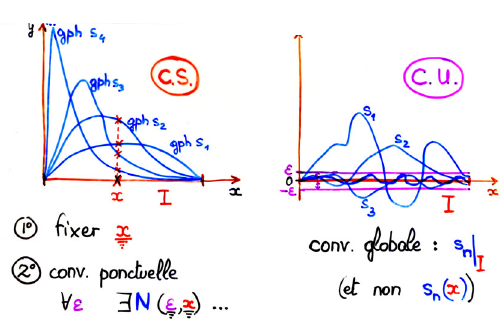
\includegraphics[scale=0.55]{image14.png}
\captionof{figure}{Convergence simple et uniforme}
\end{center}

\subsection{La norme suprémum $||\ ||_\infty$}
Dans l'espace vectoriel des fonctions bornées de $I$ dans $\mathbb{R}$ :
\begin{equation}
||\ ||_{\infty, I} : f \rightarrow ||f||_{\infty, I} := \sup\limits_{x \in I}\ |f(x)|
\end{equation}
est une norme\footnote{Elle possède bien toutes les propriétés d'une norme} : la \textit{norme suprémum}. On peut voir cette norme suprémum comme l'écart mesuré verticalement. \\
On peut re-écrire la convergence uniforme de la sorte :
\begin{equation}
\forall \varepsilon > 0, \exists N >0: \forall n \geq N :  ||s_n - S||_\infty < \varepsilon
\end{equation}

\setcounter{subsection}{4}
\subsection{Convergences de séries de fonctions}
La suite $(s_n)_{n\leq 1}$ est la \textit{suite des sommes partielles} de la série $\serie f_k$. On retrouve les implications suivantes :
\begin{itemize}
\item La série $\serie f_k$ C.S. ssi la suite $(s_n)_{n\leq 1}$ C.S.
\item La série $\serie f_k$ C.U. ssi la suite $(s_n)_{n\leq 1}$ C.U. 
\end{itemize}
Mais aussi :
\begin{equation}
\text{La série} \serie f_k\ \ \text{C.N. ($\left\{\begin{array}{l}
\text{normalement}\\
\text{en norme}
\end{array}\right.$) ssi} \serie ||f_k||_\infty \text{converge}.
\end{equation}

\setcounter{subsection}{6}
\subsection{Lien entre C.U. et C.N.}
Les critères de Cauchy pour les séries de fonctions sont les mêmes que ceux du chapitre précédent. Un corolaire liant C.U. et C.N. peut en être tiré :
\corollaire{\begin{equation}
\serie f_k\ \ \text{C.N.}\ \ \underset{\nLeftarrow}{\Rightarrow}\ \ \serie f_k\ \ \text{C.U.}
\end{equation}}

\section{Les critères de Weiestrass et d'Abel}
\subsection{Critère de Weiestrass}
Rappelons le critère de comparaison pour séries numériques:
\begin{equation}
\left.\begin{array}{l}
\forall k : |a_k| \leq M\\
\serie M_k\ \ \text{converve}
\end{array}\right\}\ \Rightarrow \serie a_k\ \ \text{C.A.}
\end{equation}

Le critère de Weiestrass n'est que l'extention du critère de comparaison, mais pour les séries de fonctions !
\begin{equation}
\left.\begin{array}{l}
\forall k : |f_k| \leq M_k\ (sur\ I)\\
\serie M_k\ \ \text{converve}
\end{array}\right\}\ \Rightarrow \serie f_k\ \ \text{C.N. sur I}
\end{equation}


\setcounter{subsection}{2}
\subsection{Critère d'Abel (pour la C.U. de séries de fonctions}
Rappelons  le critère d'Abel pour les séries numériques :
\begin{equation}
\left.\begin{array}{l}
a_k \searrow\\
|\serie \epsilon_k| \leq M
\end{array}\right\}\ \Rightarrow \serie (\epsilon_k a_k)\ \ \text{converge}
\end{equation}

Le critère d'Abel pour les séries de fonctions est donc :
\begin{equation}
\left.\begin{array}{l}
\forall x f_k(x) \searrow ; f_k  \overset{C.U.}{\rightarrow} 0 \\\
|\serie \epsilon_k(x)| \leq M
\end{array}\right\}\ \Rightarrow \serie (\epsilon_k f_k)\ \ \text{C.U.}
\end{equation}







\section{Limite uniforme d'une suite de fonctions continues}
Les sections suivantes (y compris celle-ci) sont consacrées aux qualités garanties par la convergence uniforme (d'une suite ou d'une série de fonctions). Mais avant tout , prouvons que la limite uniforme d'une suite de fonctions bornées est bornées.  
\setcounter{subsection}{-1}
\subsection{Fonction limite bornée}
\theor{Soit $\forall n \in \mathbb{N}_0, s_n : I \rightarrow \mathbb{R}$ une fonction bornée. Si $s_n \overset{C.U.}{\rightarrow} S$, alors $S$ est bornée.}
\begin{proof}
\begin{equation}
\forall \epsilon > 0, \exists N : \forall n \leq N : \sup\limits_{x \in I} |s_n - S| < \epsilon
\end{equation}
En prenant $\epsilon = 1$ et un $N(1)$, on trouve :
\begin{equation}
\forall n \leq N(1), \forall x \in I : |S(x)| < |s_n(x)|+1
\end{equation}
et donc :
\begin{equation}
\forall x \in I : |S(x)| \leq \sup\limits_{x \in I} |s_{N(1)}(x)|+1
\end{equation}
\end{proof}



\subsection{Fonction limite continue}
\theor{Soit $\forall k \in \mathbb{N}_0$, $s_k : A \subseteq \mathbb{R}^n \rightarrow \mathbb{R}$ une fonction continue.
Si $s_n \overset{C.U.}{\rightarrow} S$, alors $S$ est continue.}\ \\

\subsection{La C.U. sur tout compact suffit}
L'exemple 12.1.1 montre que si la convergence n'est pas uniforme, la continuité de la limite d'une suite de fonction continue n'est pas assurée. 
\begin{equation}
s_k : [0,1] \rightarrow \mathbb{R} : x \rightarrow x^k
\end{equation}
Si l'on restreint le domaine de cette fonction à $]0,1[$ la convergence n'est toujours pas uniforme mais la fonction limite est continue.\\
Sur tout intervalle fermé $[\eta, 1-\eta]$, la convergence est uniforme. Ceci illustre la \textbf{convergence uniforme sur tout compact inclus dans $A$} (C.U.C. sur $A$).

\subsection{Intégrale de la limite d'une suite de fonction}
\theor{Soit $A$ un compact de $\mathbb{R}^n$ dont la frontière est \textit{Riemann négligeable}, soit $\forall k \in \mathbb{N}_0, s_k : A \rightarrow \mathbb{R}$ bornée et intégrable (au sens de Riemann) si $s_n \overset{C.U.}{\rightarrow} S$, alors $\int_A S = \lim\limits_{k\rightarrow \infty} \int_A s_k$.}\ 


\section{Limite de la suite des fonctions dérivées}
\theor{Soit $\forall k\in\mathbb{N}_0:s_k\in C^p(A,\mathbb{R})$, si $\forall q=0,1,\dots,p-1:s_k^{(q)}\overset{C.S.}{\rightarrow}S_q\text{ (Notons }S:=S_0)$ et si $s_k^{(p)}\overset{C.U.}{\rightarrow}S_p$, alors $(\Rightarrow)\forall q=1,\dots,p:S^{(q)}=S_q$ et $S\in C^p$. De plus, $\forall q=0,\dots,p:s_k^{(p)}\overset{C.U.}{\rightarrow}S_q$ }\ 

\setcounter{section}{6}
\section{Continuité, intégrale, dérivées de la somme d'une série de fonctions}
\subsection{Continuité}
La somme d'une série de fonctions continues convergeant uniformément est continue.\\
Si la série C.U., la limite de sa somme vaut la somme des limites.
\subsection{Intégration}
On peut intégrer terme à terme toute série de fonctions intégrables qui converge uniformément.
\begin{equation}
\int_A \serie f_k = \serie \int_A f_k
\end{equation}

\subsection{Dérivation}
On peut dériver terme à terme toute érie de fonctions de classe $C^1$ qui converge simplement et dont la série dérivée converge uniformément sur tout compact.\\
Si la série des dérivées C.U., alors sa somme est la dérivée de la somme.

\section{Sommes de séries de puissances}
\subsection{Rayon de convergence}
A la section 11.8, nous avions vu que l'intérieur du domaine de convergence de la série 
\begin{equation}
\series c_k(z-z_0)^k
\end{equation}
avait pour \textit{rayon de convergence} dans le plan de Gauss
\begin{equation}
R := \frac{1}{\limsup\sqrt[k]{|c_k|}}
\end{equation}
La série diverge donc pour tout point en $z$ qui n'est situé ni dans le disque, ni sur son bord.

\subsection{Rayon de convergence de la série dérivée}
\theor{La série dérivée a le même rayon de convergence que la série initiale.}\ 

\corollaire{Le rayon de convergence de $\series$ est égal au rayon de convergence de $\series$ dérivées.}
\begin{proof}
\begin{eqnarray}
\sum ' := \series \frac{d}{dx}c_k(x-x_0)^k &=& \serie k c_k(x-x_0)^{k-1}\\
 &=& \series (k+1)c_{k+1}(x-x_0)^k\\
\underbrace{\limsup \sqrt[k]{(k+1)|c_{k+1}|}}_{\text{1/rayon de $\sum '$}} &=& \underbrace{\lim \sqrt[k]{k+1}}_{=1}.\limsup\sqrt[k]{|c_{k+1}|}\\
  &=& \underbrace{\limsup \sqrt[k]{|c_k|}}_{\text{1/rayon de $\sum$}}
\end{eqnarray}

\end{proof}

\subsection{CUC des séries entières}
\theor{La série $\sum := \series c_k(x-x_0)^k$ converge uniformément sur toute boule fermée incluse dans son domaine de convergence.}\

\subsection{Régularité des sommes de séries entières}
\theor{Soient $R \in \overline{\mathbb{R}}$ le rayon de convergence, $D$ le domaine de convergence et $S(x)$ la somme de la série $\series c_k(x-x_0)^k$. Alors :
\begin{enumerate}
\item $S : \text{int} D \rightarrow \mathbb{R} : x \mapsto S(x)$ est continue
\item La série dérivée $\serie kc_k(x-x_0)^{k-1}$ converge vers $S'(x)$, c'est à dire que la série initiale peut être dérivée terme à terme dans 
$B(x_0, R)$.
\item $S \in C^\infty$ et $S(x)= \series \dfrac{S^{(k)}(x_0)}{k!}(x-x_0)^k$, c'est à dire que $S(x)$ est la somme de la série de Taylor de $S$ autour de $x_0$ en tout point $x \in B(x_0,R)$.
\end{enumerate}}\ \\

Ce théorème nous montre compte que l'on peut effectuer les dérivées terme à terme et qu'en faisant ceci, on se rend compte que notre fonction peut être identifiée à sa série de Taylor.\\
\textbf{Attention !} Ceci n'est vrai que dans le domaine de convergence !\ \\
 
 Une fonction $f \in C^\infty$ est \textbf{analytique} sur $A$ ssi\footnote{$\nu_{x_0}$ est un voisinage de $x_0$.} :
\begin{equation}
\forall x_0 \in A, \exists \nu_{x_0} : \forall x \in \nu_{x_0} : f(x) = \series \dfrac{f^{(k)}(x_0)}{k!}(x-x_0)^k
\end{equation}
Comme contre-exemple, on peut prendre la fonction $f : x \rightarrow e^{-1/x^2}$ si $x \neq 0$. Dans ce cas la, le développement autour de 0 donne également 0 ($\forall x \neq 0$), ce qui est bien différent de $e^{-1/x^2}$.\\

Des fonctions comme sin, cos sont par exemple analytique. La convergence est dès lors uniforme sur tout compact et absolue sur $\mathbb{R}$.
\chapter{Intégrales généralisées, dérivations d'intégrales}
\setcounter{section}{-1}
\section{Introduction}
On est souvent en pratique confronté à des intégrales sur un domaine non borné ou dont l'intégrande n'est pas bornée. Ce ne sont donc pas des intégrales de Riemann ordinaires mais des \textit{intégrales généralisées.}\\
Trois cas vont nous intéresser ici :
\begin{enumerate}
\item $f$ varie dans le temps mais son domaine $D$ reste fixe.
\item $f$ est indépendante de $t$ mais son domaine spatial varie dans le temps.
\item Les deux bougent.
\end{enumerate}

\section{Intégrales sur un domaine constant}
Dans ce cas précis, on se pose les même questions qu'au chapitre 12 : peut on effectuer les opérations limites, dérivées et intégration librement sur une intégrale généralisée?\\
Par souci de terminologie, on dira que $x$ est la variable spatiale et que l'on intègre son domaine $D$ dans l'espace. Pareil pour $t$, cela peut être n'importe quelle valeur mais par "simplicité" on la définit comme étant le temps.

\subsection{Où limite et intégration ne permutent pas}
On ne peut pas toujours permuter l'un avec l'autre : $\lim\limits_{t \rightarrow t_0} \int_D f(x,t) dx \neq \int_D \lim\limits_{t \rightarrow t_0} f(x,t)dx$. Prenons comme exemple cette fonction (qui est la primitive de la dérivée ci-contre) :
\begin{equation}
f(x,t) := \frac{x^2 - t^2}{(x^2+t^2)^2} = \frac{\partial}{\partial x} \left(\frac{-x}{x^2+t^2}\right)\ \ \ \ \ \ pour(x,t) \neq (0,0)
\end{equation} 
En effectuant les permutations, on confirme le résultat prédit.
\begin{itemize}
\item $\lim\limits_{t \rightarrow 0} \int_0^1 f(x,t) = -1$
\item $\int_0^1 \lim\limits_{t \rightarrow 0} f(x,t) = +\infty$
\end{itemize}
Ceci est du au fait que $f$ est \textit{non bornée} au voisinage de (0,0) et qu'elle est continue sur $([0,1]\times[0,1])\backslash\{0,0)\}$) ce qui n'est pas un compact !\\

\subsection{Passage à la limite sous le signe intégral}
Pour passer la limite sous le signe intégral, il faut que $f$ soit \textbf{continue sur un compact}\footnote{Un compact est un ensemble fermé et borné. Une fonction sur un compact atteint ses bornes et est uniformément continue.}.
\theor{
\begin{equation}
\lim\limits_{t \rightarrow t_0, t \in T_0} \int_D f(x,t) dx = \int_D \lim\limits_{t \rightarrow t_0, t \in T_0} = \int_D f(x,t_0)dx
\end{equation}
si :$\left\{\begin{array}{l}
D \text{est un compact mesurable}\\
T_0 \text{est un compact et $t_0 \in T_0$.}\\
f \text{est continue sur $D \times T_0$}
\end{array}\right.$
}\ \\

\corollaire{Ce résultat est aussi valable si :\\
si :$\left\{\begin{array}{l}
D \text{est un compact mesurable et $t_0 \in\ $int$\ T  \subseteq\mathbb{R}$.}\\
f \text{est continue sur $D \times T$}
\end{array}\right.$
}\ \\

\corollaire{
\begin{enumerate}
\item Si $D$ est un compact mesurable, $T$ est un compact et que $f$ est continue sur $D \times T$, alors la fonction $I(t) := \int_D f(x,t)dx$ est continue sur $T$.
\item Si $D$ est un compact mesurable et $f$ est continue sur $D \times T$, alors la fonction $I$ est continue sur int $T$.
\end{enumerate}}


\subsection{Dérivation sous le signe intégral}
Si $D$ est fixé, il est forcément indépendant de $t$. Il me suffit dès lors de dériver sous le signe intégrale\footnote{La démo est dans le syllabus (p.6) pour "ceux qui aiment ça".} :\\

\theor{
\begin{equation}
\frac{d}{dt}\int_D f(x,t) dx = \int_D \frac{\partial f}{\partial t}(x,t) dx
\end{equation}
si : $\left\{\begin{array}{l}
D \text{est un compact mesurable}\\
f\ et\ \frac{\partial f}{\partial t} \text{sont continues sur $D \times T$}
\end{array}\right.$}

\subsection{Intégration sous le signe intégral}
En reprenant le même exemple que précédemment, on se rend compte que l'on ne peut permuter les intégrales. Cela semble contredire le \textit{théorème de Fubini} mais ce n'est pas le cas : en réalité l'intégrale double n'existe pas car on ne travaille pas sur un compact (on a exclu (0,0)). 

\section{Intégrales sur un domaine variable}
Nous allons maintenant considéré le cas ou $f$ est indépendante de $t$, mais pas le domaine. Dans la suite, on considèrera que le "domaine grandit avec $t$" (et donc que le bord du domaine bouge).

\subsection{Continuité par rapport au domaine d'intégration}
Supposons que $D_t$ est mesurable compact $\forall t \in T$ et qu'il croît lorsque $t$ augmente. Dans ce cas, nous avons :\\
\theor{$I(t) := \int_{D_t} f(x)dx$ est continue sur tout compact $\subset T$.}
\begin{proof}(pas connaitre)\\
Considérons l'accroissement $I(t_0 + \Delta t) - I(t_0)$ :
$$|\Delta I| = \left|\int_{D_{t_0 + \Delta t}} f - \int_{D_{t_0}}\right| = \left|\int_{\Delta D} f \right| \leq \mu(\Delta D).\sup\limits_{D_M}|f|$$
où $D_M$ est un compact $\supseteq D$.
\end{proof}

\subsection{Règle de Leibniz en $1D$}
Lorsque $D_T := [a,t]$\footnote{Cela signifie que la bord du domaine progresse à vitesse unité.}, on retrouve le résultat fondamental de la règle de Leibniz (Ch.9) :
\begin{equation}
\frac{d}{dt}\int_a^t f(x)dx = f(t)
\end{equation}
Si le domaine progresse en fonction de $\psi(t) : D_t := [a, \psi(t)]$. Nous avons dans ce cas : 
\begin{equation}
\frac{d}{dt}\int_a^{\psi(t)} F(x) dx = F'(\psi(t)).\psi'(t)
\end{equation}


\subsection{Règle de Leibniz en $2D$}
Si seul le domaine variée, la dérivée par rapport à $t$ de cette intégrale c'est la limite pour $\Delta t \rightarrow 0$ du quotient différentiel :
\begin{equation}
\frac{d}{dt} \iint_{D_t} f(x,y) dxdy = \lim\limits_{\Delta t \rightarrow 0} \dfrac{\iint_{t + \Delta D} f(x,y) dxdy - \iint_{D_t} f(x,y)dxdy}{\Delta t} =\  ?
\end{equation}
\begin{wrapfigure}[10]{r}{3cm}
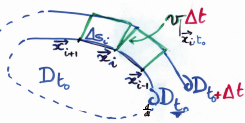
\includegraphics[scale=0.7]{image16.png}
\captionof{figure}{Décomposition du domaine}
\end{wrapfigure}
Supposons qu'on connaisse en chaque point la vitesse de variation du domaine. On va approcher l'aire de la couronne par la somme d'aire de petits pavés à l'aide d'une ligne polygonale. \\

Je nomme $\Delta s_i$ la longueur d'une telle arrête de ma ligne et la vitesse de la frontière du domaine progresse à vitesse $v$.\\
La progression sur le temps $\Delta t$ sera dès lors $v.\Delta t$. Comme j'approche $f$, je dois chaque fois le multiplier par les approximations d'aires\footnote{Je note $\vec{x} = (x,y)$ et $d\vec{x} = dxdy$.} :
\begin{equation}
\dfrac{\iint_{\Delta D} f(\vec{x})d\vec{x}}{\Delta t} \approx \sum_i f|_{\vec{x_i}}v|_{\vec{x_i}}\Delta s_i \ \ \ \ \rightarrow \oint_{\partial D_{t_0}}fv\ ds
\end{equation}
En faisant tendre $\Delta s_i \rightarrow 0$ j'obtiens comme limite l'intégrale curviligne de $f.v$ sur le bord $\partial D_{t_0}$.
On a donc la fameuse \textbf{formule de Leibnitz}\footnote{Terminologie utilisée par les ingénieurs} :
\begin{equation}
\frac{d}{dt}\iint_{D_t} f(x,y) dx dy = \oint_{\partial D_t}fv\ ds
\end{equation}

\subsection{Leibniz sur des domaines $D_t \equiv h(x,y) <t$}
Imaginons par exemple un domaine de rayon $t$ variant à vitesse unité $\vec{1_r}\ (= \vec{\nabla}h)$ :
\begin{equation}
D_t := B(\vec{0},t) \equiv \underbrace{\sqrt{x^2 + y^2}}_{h(x,y)} < t
\end{equation}
Dans le cas particulier ou $f=1$ :
\begin{equation}
\frac{d}{dt}\iint_{D_t} 1 = \oint_{C_t} 1 ds
\end{equation}
On retrouve que la dérivée de l'aire d'un disque de rayon $t$ vaut le périmètre de ce disque !\\

En prenant $h = t$ on défini un ensemble de niveau de $h$ qui est à priori le bord du domaine. Le gradient de $h$ est perpendiculaire à la courbe de niveau et pointe du côté ou $h$ augmente.\\
On se rappelle que $\vec{\nabla}h$ donne la plus grande pente et que sa norme donne la vitesse de cette plus grande pente (et que le vecteur unitaire gradient donne la direction du plus grand accroissement de $h$ (toujours en un point)). \\
On peut dire que :
\begin{equation}
\frac{\Delta h}{||(\Delta x, \Delta y)||} \approx ||\vec{\nabla}h||_{(x,y)}
\end{equation}
En supposant que $\Delta h = \Delta t$\footnote{Car vitesse unitaire ? A vérif.}, on trouve :
\begin{equation}
\frac{||(\Delta x, \Delta y)||}{\Delta t} \approx \frac{1}{||\vec{\nabla}h||} = v
\end{equation}
La formule de Leibniz devient dans ce cas :
\begin{equation}
\frac{\partial}{\partial t} \iint_{D_t} f(x,y) dxdy = \oint_{\partial D_t} \dfrac{f}{||\vec{\nabla}||}ds
\end{equation}

\subsection{Bord mouvant := partie du bord qui varie}
Pour pouvoir écrire la formule de façon plus générale, il arrive que l'on travaille dans un certain secteur par exemple le secteur A. Le bord mouvant est la partie qui "varie",le reste du bord ne varie pas.\footnote{Oublier l'astérisque = FAUX !}
\begin{equation}
\frac{\partial}{\partial t} \iint_{D_t} f(x,y) dxdy = \oint_{\partial * D_t} \dfrac{f}{||\vec{\nabla}||}ds
\end{equation}

\subsection{Leibniz en $3D$}
C'est la même chose, mais avec des intégrales de surface et de volume :
\begin{equation}
\frac{d}{dt} \iiint_{h(x,y,z) < t} f(x,y,z)dxdydz = \iint_{h(x,y,z) = t} \frac{f}{||\vec{\nabla}h||}d\sigma
\end{equation}

\subsection{Domaine et intégrande variant indépendamment}
C'est le dernier cas à traiter, celui ou $f$ et $D$ dépendent de $t$.\\
Pour simplifier les choses, on va inclure une troisième variable $u$ (on aura alors $t, x$ et $u$). L'avantage est que l'on "fixera" la dérivée partielle par rapport à $t$ pour chaque composante à son tour :\\

\theor{Si $F(t,u) := \int_{D_t} f(x,u) dx$ avec comme  hypothèse que $f$ est continue sur $D \times U$, alors:
\begin{enumerate}
\item $F$ est continue sur $T \times U$
\item $\dfrac{\partial}{\partial t}\int_{h(x) < t} f(x,u) dx = \oint_{h(x) = t} \dfrac{f(x,u)}{||\vec{\nabla} h|_x||}ds$
\item $\dfrac{\partial}{\partial  u}\int_{D_t} f(x,u) dx = \int_{D_t} \frac{\partial f}{\partial u} (x,u) dx$
\end{enumerate}
}\ \\

Dans le deuxième cas, on "fixe" $f$ dans le temps et l'on utilise la formule de Leibniz lorsque seul le domaine varie et dans le troisième cas, seul $f$ dépend de $t$ : il suffit de dériver sous le signe intégrale.

\subsection{Règle de Leibniz pour $\int_{D_t} f(x,t) dx$}
La borne supérieur et inférieur dépend de $t$ : la dérivée se calcule en tenant compte séparément de chaque cas :
\begin{equation}
\frac{d}{dt}\int_{\phi(t)}^{\psi(t)} f(x,t) =  \frac{d}{dt}\left[\int_c^{\psi(t)}f(x,t) - \int_c^{\phi(t)}f(x,t)\right]
\end{equation}
Mais encore :
\begin{equation}
\frac{d}{dt}\int_{\phi(t)}^{\psi(t)} f(x,t) = \int_{\phi(t)}^{\psi(t)} \frac{\partial f}{\partial t}(x,t) + f|_{(\psi(t),t)} \psi'(t) - f|_{(\phi(t), t)}
\end{equation}

L'idée est toujours la même : introduire des variables auxiliaires pour traiter une difficulté à la fois.
\begin{equation}
\frac{d}{dt}\int_{D_t} f(x,t) dx = \int_{D_t} \frac{\partial f}{\partial t}(x,t) + \int_{\partial D_t} \frac{f(x,t)}{||\vec{\nabla}h||}ds
\end{equation}


\chapter{Séries de Fourier}
\section{Introduction}
\subsection{Approche locale d'une fonction par Taylor}
La série de Taylor est une approche \textit{locale} près d'un point $x_0$, relatives aux puissances $(x-x_0)^k : \sum^\infty c_k(x-x0)^k$ et à la troncature $\mathcal{O}((x-x_0)^n)$.

\subsection{Approche globale d'une fonction par Fourier}
Ici on travaille sur un intervalle (un domaine déterminé) on cherche une forme de développement de la fonction qui traduise plutôt son comportement global sur $I$ tout entier : c'est le développement de Fourier.\\
Cette série donne une approche globale relativement aux fonctions $\phi_k(x) : \sum^\infty c_k\phi_k(x)$.

\section{Systèmes orthonormés de fonctions}
\setcounter{subsection}{-1}
\subsection{Rappel : base orthonormée dans espace vectoriel $V$}
Une base $(\vec{e_k})$ est orthonormée s'il existe une et une seule décomposition de $\vec{v}$ tel que:
\begin{equation}
\vec{v} = \sum_{k\in \mathbb{K}} c_k\vec{e_k}
\end{equation}
et si :
\begin{itemize}
\item $V$ est muni du produit scalaire dans lequel $(\vec{e_k})$ est orthonormée
\end{itemize}
Sinon il faudra orthogonaliser la base (Gram-Schmidt)

\subsection{Dans un espace vectoriel muni d'un produit scalaire (espace préhilbertien)}
On défini un produit scalaire particulier pour Fourier :
\begin{equation}
\left\{\begin{array}{l}
\text{Produit scalaire}\ \ \ \ \langle f,g \rangle := \int_a^b f.g\\
\text{Produit hermitien} \ \langle f,g \rangle := \int_a^b f.g^*
\end{array}\right.
\end{equation}
La norme sera quant à elle définir par : 
\begin{equation}
||f|| = \sqrt{\int_a^b |f|^2} = \sqrt{\langle f,f\rangle}
\end{equation}
\subsection{"La" classe $L^2$}
La classe $L^2[a,b]$ est la classe des fonctions de carrés sommables (ou "intégrables"), c'est à dire des fonctions $f$ définies et intégrales sur $[a,b]$ telles que (au cas ou il s'agit d'une intégrale généralisée) :
\begin{equation}
\int_a^b |f|^2 < +\infty
\end{equation}
Cette appellation vient du fait que \textit{l'intégralité de $f^2$ entraine l'intégrabilité de $f$ sur $[a,b]$} ce qui est vrai en considérant l'intégrale de Lebesgue.\\
Ceci est aussi vrai si la fonction est localement intégrable sauf en un nombre fini de pôles\\

\retenir{Si $f$ a un pôle en $a^+$ mais $\left\{\begin{array}{l}
bornée\\
intérable\ sur\ tout\ [a,b]
\end{array}\right.$ alors

\begin{equation}
\int_{a^+}^b |f|^2 < +\infty  \Rightarrow \int_{a^+}^b |f| < +\infty \Rightarrow \int_{a^+}^b f\ \text{converge}
\end{equation}}
$\langle , \rangle$ est bien définir sur $L^2$ (démonstration pas à connaître.)\\
Néanmoins, un point pose problème : $\langle f,f \rangle \geq 0 \Rightarrow f = 0$. Ceci n'est pas toujours vrai, si l'intégrale de $f^2$ est nulle cela n'implique pas que $f$ est toujours nulle\footnote{La fonction 1 si $x=0$ et 0 si $x\neq 0$ à une intégrale nulle mais n'est pas rigoureusement nulle}.\\

On dira alors que $f$ vaut "presque partout zéro". $\langle f,f \rangle$ est un vrai produit scalaire sur $C^0([a,b])$ mais comme $C^0$ est trop restrictif on dira que $\langle f,f \rangle$ est "presque" un produit scalaire sur $L^2$ et on identifiera les fonctions comme "presque égales".
\setcounter{subsection}{4}
\subsection{Systèmes libres, orthogonaux, orthonormés}
Soit $\Phi =  \{\phi_j\ |\ j \in \mathbb{N}\}$ un ensemble dénombrable (dit \textit{système}) de fonction de $L^2([a,b], \mathbb{C})$.\\
$\Phi$ est un système
\begin{description}
\item[Libre] si toute parties finie de $\Phi$ est libre 
\item[Orthogonal] si $j \neq k \rightarrow \langle \phi_j, \phi_k \rangle = 0$
\item[Orthonormé] si $\langle \phi_j, \phi_k \rangle = \delta_{ij}$
\end{description}


\section{Définition des séries de Fourier relativement à  un système orthonormé}
On travaille dans l'EV $L^2([a,b],\mathbb{K})$ où le produit scalaire est défini par :
\begin{equation}
\langle f,g \rangle_p = \int_a^b fg^*p
\end{equation}
où $p$ est une fonction poids.\\
$L^2$ devient ainsi un \textit{espace pré-hilbertien}. On définit $\Phi$ comme précédemment, c'est à dire un système orthogonal de vecteur de $L^2$. Attention, ce n'est pas forcément une base !! Il n'est pas forcément assez fourni\footnote{En effet, $L^2$ est infini non-dénombrable}.

Par exemple si on prend un système simple comme les monômes : $\phi_k(x) = x^k (k =0,1,\dots)$. Si on considère l'EV engendré parles monômes on obtiendra l'ensemble des polynômes. Par contre, on considèrera les séries entières des sommes infinies.

\retenir{Soit $\Phi$ un système orthogonal dans $L^2([a,b])$. Soit $f \in L^2([a,b], \mathbb{K})$.\\
La série de Fourier de $f$ relativement à $\Phi$ est :
\begin{equation}
f \sim \series \dfrac{\langle f, \phi_k \rangle}{\langle \phi_k, \phi_k \rangle}\phi_k
\end{equation}}
Les $c_k = \frac{\langle f, \phi_k \rangle}{\langle \phi_k, \phi_k \rangle}$ sont appelées \textit{coefficients de Fourier de $f$} relativement à $\Phi$.
\setcounter{subsection}{1}
\subsection{Trois types usuels de convergence d'une suite ou d'une série de fonctions}
Convergence Simple ($C.S.$) : $$\series f_k\overset{C.S.}{=}f\Leftrightarrow\forall x\in [a,b]:\left|\sum_{k=0}^nf_k(x)-S(x)\right|\overset{n\rightarrow\infty}{\rightarrow}0$$
Convergence uniforme ($C.U.$) : $$\series f_k\overset{C.U.}{=}f\Leftrightarrow\sup_{x\in [a,b]}\left|\sum_{k=0}^nf_k(x)-S(x)\right|\overset{n\rightarrow\infty}{\rightarrow}0$$
Convergence en moyenne quadratique ($C.L^2$) : $$\series f_k\overset{L^2}{=}f\Leftrightarrow\int_a^b\left|\sum_{k=0}^nf_k(x)-S(x)\right|^2\,dx\overset{n\rightarrow\infty}{\rightarrow}0$$
\begin{center}
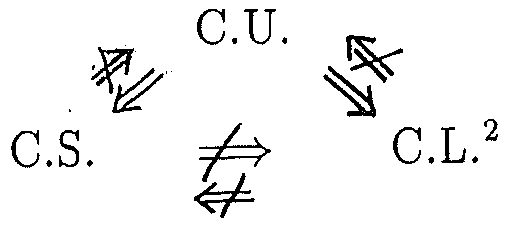
\includegraphics[scale=0.3]{CSCUCL}
\captionof{figure}{Lien entre ces différents types de convergence}
\end{center}
\setcounter{subsection}{3}
\subsection{Calcul des coefficients de Fourier en cas de C.U.}
\theor{Si $\{\phi_k\}_{k \in \mathbb{N}}$ est orthogonal et si $\serie c_k\phi_k$ converge uniformément vers $f$, alors 
\begin{equation}
c_k = \dfrac{\langle f, \phi_k \rangle}{\langle \phi_k, \phi_k \rangle}
\end{equation}}
\begin{proof}
\ \\
Par hypothèse $f = \serie c_j\phi_j$.\\
Calculons le produit scalaire en considérant un poids de 1 :
\begin{equation}
\langle f, \phi_k\rangle = \int_a^b \left(\serie c_j\phi_j \right)\phi_k^*
\end{equation}
$\phi_k$ multiplie chacun des termes de la série
\begin{equation}
\langle f, \phi_k\rangle = \int_a^b \serie c_j\phi_j\phi_k^*
\end{equation}
Comme nous avons convergence absolue, on peut calculer terme à terme et permuter sommation et intégration.
\begin{equation}
\langle f, \phi_k\rangle = \serie c_j \int_a^b \phi_j\phi_k^*
\end{equation}
Sachant que $\phi_j\perp \phi_k$ si $j\neq k$ on peut ré-écrire :
\begin{equation}
\langle f, \phi_k\rangle = \serie c_j\delta_{jk} \int_a^b |\phi_k|^2
\end{equation}
Ou encore :
\begin{equation}
\langle f, \phi_k\rangle = c_k\langle \phi_k, \phi_k\rangle
\end{equation}
Donc :
\begin{equation}
c_k = \dfrac{\langle f, \phi_k \rangle}{\langle \phi_k, \phi_k \rangle}
\end{equation}
\end{proof}

\section{Coefficients des séries de Fourier classiques}
\subsection{Série sinus et cosinus sur $L^2([-\frac{T}{2}, \frac{T}{2}], \mathbb{R})$}
Comme la période est $2/\pi$ on peut travailler sur tout  intervalle de cette taille. Comma la période est $T$, autant la centrer sur l'origine.
\begin{equation}
\Phi = \left\{ \frac{1}{2}, \cos\left(\frac{2k\pi}{T}x\right), \sin\left(\frac{2k\pi}{T}x\right) ; k \in \mathbb{N}_0\right\}
\end{equation}
Le développement de Fourier de $f$ :
\begin{equation}
f(x) \sim \frac{a_0}{2} + \serie (a_k\cos(k\omega_0x) + b_k\sin(k\omega_0x))
\end{equation}
où $\omega_0$ est la \textit{pulsation fondamentale} et :
\begin{equation}
\left\{\begin{array}{l}
a_k = \frac{2}{T}\int_{-T/2}^{T/2} f(u)\cos\left(\frac{2k\pi}{T}u\right)du\\
b_k = \frac{2}{T}\int_{-T/2}^{T/2} f(u)\sin\left(\frac{2k\pi}{T}u\right)du
\end{array}\right.
\end{equation}

\subsubsection{Forme exponentielle pour une fonction réelle}
A l'aide de l'expression du sinus et cosinus en nombre complexe, on peut écrire 
\begin{equation}
f \sim \sum_{k=-\infty}^\infty c_ke^{ik\omega_0x}
\end{equation}
où $c_k = \dfrac{a_k - ib_k}{2}$.

\subsection{Série sinus dans $L^2([0, L], \mathbb{R})$} 
\begin{equation}
\Phi = \left\{\sin\left(\frac{k\pi}{T}x\right) ; k \in \mathbb{N}_0\right\}
\end{equation}
\begin{equation}
b_k=\frac{2}{L}\int_0^Lf(x)\sin\left(\frac{k\pi}{T}x\right)\,dx
\end{equation}
\subsection{Série cosinus dans $L^2([0, L], \mathbb{R})$} 
\begin{equation}
\Phi = \left\{\cos\left(\frac{k\pi}{T}x\right) ; k \in \mathbb{N}_0\right\}
\end{equation}
\begin{equation}
a_k=\frac{2}{L}\int_0^Lf(x)\cos\left(\frac{k\pi}{T}x\right)\,dx
\end{equation}

\subsection{Série de Fourier complexe de $f$}
Le développement en série de Fourier de $f :[-T/2; T/2] \rightarrow \mathbb{C}$ est donné par :
\begin{equation}
f \sim \sum_{k=-\infty}^\infty c_ke^{ik\omega_0x}
\end{equation}
où :
\begin{equation}
c_k = \dfrac{\langle f(x), e^{ik\omega_0x}\rangle}{\langle e^{ik\omega_0x}, e^{ik\omega_0x} \rangle}
\end{equation}
On voit donc qu'il n'y a nul besoin de passer par la trigonométrie pour écrire un développement de Fourier sous forme exponentielle.

\subsection{Partie inconnue}
\retenir{La projection de $f$ sur $\phi_k$ est $c_k\phi_l$ où $c_k$ est le coefficient de Fourier de $f$ relativement à $\phi_k$, i.e. le coefficient de $\phi_k$ dans le développement de Fourier de $f$ :
\begin{equation}
proj_{\phi_k}(f) = \dfrac{\langle f, \phi_k \rangle}{\langle \phi_k, \phi_k \rangle}\phi_k
\end{equation}
}\ \\
Regardons dans notre espace à $n$ dimension et prenons sa projection : on travaille dans un espace $n+1$.
\begin{center}
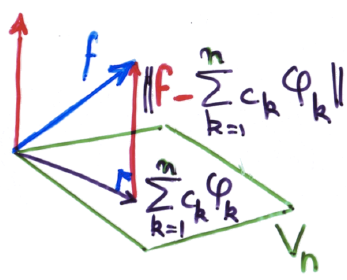
\includegraphics[scale=0.55]{image17.png}
\captionof{figure}{Projection}
\end{center}
La projection vaut $||f - \sum_{k=1}^n a_k\phi_k||$. En repant la norme (pythagore), on trouve :
\begin{equation}
||f||^2 = \sum_{k=1}^n |c_k|^2||\phi_k||^2 + R_n^2\ \ \ \text{où}\ R_n = ||f - \sum_{k=1}^n a_k\phi_k||
\end{equation}

\retenir{La meilleure approximation en moyenne quadratique $(L^2)$ de $f$ sur $\Phi_n$ est le vecteur $\sum_{k=1}^n a_k\phi_k$ de $\Phi$ qui minimise :
\begin{equation}
\left|\left| f - \sum_{k=1}^n a_k\phi_k \right|\right|_2
\end{equation}
Les coefficients $a_k$ réalisant la meilleure approximation en moyenne quadratique de $f$ sur $\Phi_n$ sont les n premiers  coefficients de Fourier de f par rapport à $\Phi$.\\
 La meilleure approximation en moyenne quadratique de $f$ relativement à $\Phi_n$ est le
développement limité (de Fourier) à l'ordre $n$ de $f$.\\

Lorsque le système partiel $\Phi_n$ croît (lorsque $n$ augmente), il suffit d'ajouter des termes au développement (et non de recalculer tous les coefficients)}

\section{Bessel, Parseval, complétude et conv. $L^2$}
\subsection{Inégalité de Bessel}
La suite des coefficients de Fourier tend vers zéro. Si le système est orthonormé, on obtient une égalité qui est l'\textit{inégalité de Bessel}. Elle découle de l'égalité $||f||^2 = \sum_{k=1}^n |c_k|^2||\phi_k||^2 + R_n^2 \Rightarrow \sum_{k=1}^n |c_k|^2||\phi_k||^2 \leq ||f||^2$.\\

\theor{Soit $\Phi$ un système orthogonal de fonctions de $L^2$. Soit $f \in L^2$ et soit $c_k$ le coefficient de Fourier de $f$ relativement à $\phi_k$. Il tient 
\begin{equation}
\serie |c_k|^2||\phi_k||^2 \leq ||f||^2
\end{equation}}\ \\
\corollaire{Si le système est orthonormé, il s'ensuit :
\begin{equation}
\serie |c_k|^2||\phi_k||^2 \leq \infty
\end{equation}}

\subsection{Théorème de Parseval}
Pour rappel, $R_n$ est la distance de $f$ à $\Psi_n$ et en particulier $R_n$ décroit lorsque $n$ augmente.
\begin{equation}
R_n \rightarrow 0 \Leftrightarrow \series |c_k|^2||\phi_k||^2 = ||f||^2
\end{equation}
En effet : $R_n^2 = ||f - \sum_{k=1}^n c_k\phi_k||^2 = \int_a^b |f - \sum_{k=1}^n c_k\phi_k|^2 \rightarrow 0 \Leftrightarrow f = \series |c_k|^2||\phi_k||^2 = ||f||^2$.\\
On voit que cette série converge et converge exactement vers la norme de $f$ si et seulement si la série de fourier converge en moyenne quadratique.\\

\theor{Si $f_{L^2} = \serie c_k\phi_k$ alors $\serie |c_k|^2||\phi_k||^2 \leq ||f||^2$}\ \\

On définit ça comme "complet" ssi la série de Fourier de $f$ relativement à un tel système converge en moyenne quadratique et ce pour tout $f$.\\

Par \textbf{définition}, le système orthogonal $\Phi$ est \textit{complet dans $L^2([a,b])$ ssi $f \overset{L^2}{=}\serie c_k\phi_k$ pour tout $f \in L^2$}.


\subsubsection*{Unicité de la décomposition}
Si la fonction $f = 0$ c'est parce que $f$ est orthogonale à tous le s$\phi_k$, donc tous les $c_k$ seront nuls. Par Parseval, la norme de $f$ devrait être nulle, mais on sait que $f$ ne sera réellement null que si $f$ est continue.\\

\retenir{Dans un système orthogonal $\Phi$ complet sur $L^2([a,b])$, si $f \in L^2$ est tel que $f \perp \phi_k \forall k \in \mathbb{N}_0$, alors $||f||=0$. Si  de plus $f\in C^0$, alors $f=0$ sur $[a,b]$.}\ \\

\begin{proof}
Par l'égalité de Parseval :
\begin{equation}
||f||^2 = \series |c_k|^2||\phi_k||^2  = 0,\ \text{i.e. }\ \int_a^b |f|^2 = 0
\end{equation}
\end{proof}

\corollaire{Soit le système orthogonal $\Psi$ complet sur $L^2([a,b])$, si $c_k(f) = c_k(g) \forall k \in \mathbb{N}_0$, alors $f=g$ presque partout, c'est à dire $\int_a^b |f-g|^2 = 0$.}\ \\
Cela signifie que les coefficients de Fourier déterminent univoquement leur fonction génératrice.\\


\retenir{Si deux séries de Fourier convergent (au sens $L^2$) vers une même fonction, alors, celles-ci sont égales}\ \\
\begin{proof}
\begin{equation}
\series c_k\phi_k = f\ \ \text{et}\ \ \series d_k\phi_k = f\ \ \Rightarrow \series (c_k-d_k)\phi_k = 0
\end{equation}
En appliquant l'égalité de Parseval, on trouve : 
\begin{equation}
\series |c_k-d_k|^2||\phi_k||^2 = 0 \Rightarrow c_k = d_k \forall k \in \mathbb{N}_0
\end{equation}
\end{proof}
\setcounter{subsection}{3}
\subsection{Meilleure approximation en moyenne quadratique de $f$ dans $V_n$}
Les coefficients $a_k$ qui réalisent la meilleure approximation en moyenne quadratique ($L^2$) de $f$ relativement à $\Phi|_{\leq n}$ sont les $n+1$ premiers coefficients de Fourier de $f$ relativement à $\Phi$
\begin{proof}\ \\
Il faut $a_k$ qui minimise l'erreur quadratique $\left\|f-\sum_{k=0}^na_k\phi_k\right\|_2$ \begin{align*}
 & \Rightarrow \left\|f-\sum_{k=0}^na_k\phi_k\right\|_2^2=\left<f-\sum_{k=0}^na_k\phi_k,f-\sum_{k=0}^na_k\phi_k\right>\\
 & =\left<f,f\right> - \sum_{k=0}^na_k^*\left<f,\phi_k\right>- \sum_{k=0}^na_k\left<\phi_k,f\right> + \sum_{j,k=0}^na_ka_j^*\left<\phi_k,\phi_j\right>\\
 & = \underbrace{\left<f,f\right>}_{donné}+\sum_{k=0}^n\underbrace{(c_k-a_k)(c_k^*-a_k^*)}_{\geq 0}-\underbrace{\sum_{k=0}^nc_kc_k^*}_{donné}
\end{align*}
Donc $\left\|f-\sum_{k=0}^nc_k\phi_k\right\|_2^2$ est minimum $\Leftrightarrow \forall k=0,\dots,n : c_k=a_k$
\subsubsection{Remarque}
Soit $V_n=\text{vect}\{\phi_0,\dots,\phi_n\}$, le vecteur de $V_n$ le plus proche de $f$ est la projection orthogonale de $f$ sur $V_n$ $$\text{proj}_{V_n}f=\sum_kc_k\phi_k\quad\text{où}\quad c_k:=\text{ coef. de Fourier def. relativement à }\phi_k$$
\end{proof}
\section{Fonctions régularisées}
\subsection{Fonction régularisée}
S'il existe une subdivision de $[a,b]\,|\,f$ est continue sur chaque subdivision et que sur chaque borne de cette subdivision, la limite à gauche et à droite existent, alors $f$ est continue par morceaux sur $[a,b]$. On peut alors la régulariser $$\tilde{f}=\left\{\begin{array}{l}
\frac{f(x^-)+f(x^+)}{2}\quad x\in ]a,b[\\
\frac{f(a^+)+f(b^-}{2}\quad x=a\text{ ou }x=b
\end{array}\right.$$ $\tilde{f}$ étant la fonction régularisée de $f$, les \textit{points réguliers} sont les points tels que $f=\tilde{f}$\\ On définit aussi un prolongement périodique de $\tilde{f}$ (période $b-a$) : $\tilde{f}_{pro}$. Si $\tilde{f}_{pro}$ est continue sur $[a,b]$ alors $\tilde{f}$ et $f$ sont continue par morceaux.
\section{Convergence simple des séries classiques}
\subsection{Théorème de Dirichlet}
\theor{Si $f$ et $f'\in C_{morc}^0[-\pi,\pi]$, alors $$\frac{a_0(f)}{2}+\serie(a_k(f)\cos(kx)+b_k(f)\sin(kx))\overset{C.S.}{=}\frac{f(x^+)+f(x^-)}{2}$$ c-a-d que la \textit{série de Fourier de f converge vers la régularisée de f}}\ \\
\corollaire{Si $\tilde{f}_{proj}\in C^0(\mathbb{R})$ et $f'\in C^0_{morc}[-\pi,\pi]$, alors $\sum\limits^{\infty}\ Fourier\ class.(f)\overset{C.S.}{=}f_{proj}(x)$}
\section{Théorèmes de convergence uniforme}
\subsection{Convergence uniforme des séries classiques}
pp.53--55

\setcounter{chapter}{15}
\chapter{EDL - Problèmes aux limites et fonctions propres}
\section{Problèmes aux limites linéaires pour EDL}
\subsection{Conditions aux limites linéaires}
On recherche parmis les solutions $y$ d'une ED d'ordre $n$ celles qui sont de classe $C^n$ sur $[a,b]$ et satisfont à une condition qui porte sur les valeurs de $y,y',\dots,y^{(n-1)}$ au bord du domaine $[a,b]$, c'est à dire en $a$ et en $b$, parfois appelés "limites" du domaine.


\subsection{Conditions aux limites séparées}
Il existe trois cas particulier pour une EDL d'ordre 2 sur $[a,b]$ :
\begin{enumerate}
\item \textbf{CL de Dirichlet} ; impose $y$ sur le bord du domaine. En version homogène (CLH) :
\begin{equation}
\left\{\begin{array}{l}
y(a) = 0\\
y(b) = 0
\end{array}\right.
\end{equation}
\item \textbf{CL de Neumann} ; impose $y'$ sur le bord du domaine. En version homogène (CLH) :
\begin{equation}
\left\{\begin{array}{l}
y'(a) = 0\\
y'(b) = 0
\end{array}\right.
\end{equation}
\item \textbf{CL périodique} ; de période $b-a$. En version homogène ;
\begin{equation}
\left\{\begin{array}{l}
y(a)-y(b) = 0\\
y'(a) - y'(b) = 0
\end{array}\right.
\end{equation}
\end{enumerate}
\subsubsection{Espace vectoriel}
Considérons les conditions aux limites homogènes pour une EDL d'ordre 2 sur $[a,b]$
\begin{equation}
\left\{\begin{array}{l}
cl_a(y) := \alpha_0y(a) + \alpha_1y'(a) = 0\ \ \ \ \ (CL_a)\\
cl_b(y) := \beta_0y(b) + \beta_1y'(b) = 0\ \ \ \ \ (CL_b)\\
\end{array}\right.
\end{equation}
où $\alpha_i,\beta_i \neq 0$. Les différents espaces associés sont :
\begin{itemize}
\item L'EV des fonctions satisfaisant $CL_a$ est un hyperplan de $C^2\ ([a,b], \mathbb{R})$
\item L'espace des solution de l'EDLH est de dimension 2.
\item L'espace des solution de l'ELDH satisfaisant à $CL_a$ est de dimension 1
\item L'espace des solutions de l'EDLH satisfaisant à $CL_a$ et $CL_b$ est de dimension 0 ou 1
\end{itemize}
Ce résultat se généralise simplement ($cl_i$ est une application linéaire).

\subsection{Problème homogène}
Soit $L$, un opérateur différentiel régulier d'ordre $n$ ainsi que les conditions au limites linéaires homogènes $cl_i(y) =0\ (i=1,\dots,n)$. On cherche à résoudre
\begin{equation}
\left\{\begin{array}{ll}
L(y) &=0\\
cl_i(y) &= 0
\end{array}\right.
\end{equation}
Soit $y_1,\dots,y_n$, $n$ solutions linéairement indépendantes de l'EDLH (c'est à dire telles que $W(y_1,\dots,y_n)\neq 0$, on a donc un système fondamental). La solution peut s'écrire
\begin{equation}
y = c_1y_1 + \dots + c_ny_n\ \ \ \text{où}\ c_i \in \mathbb{R}
\end{equation}
Il faut donc trouver les $c_i$ tels que les conditions aux limites soient satisfaites, c'est-à-dire :
\begin{equation}
cl_i(c_1y_1 + \dots + c_ny_n) = 0
\end{equation}
Ce qui donne, par linéarité des conditions aux limites homogènes (CLH)
\begin{equation}
c_1cl_i(y_1) + \dots + c_ncl_1(y_n) = 0
\end{equation}
On peut en construire un système algébrique linéaire homogène en les $c_i$ de matrice
\begin{equation}
Mcl(y_1, y_2, \dots, y_n) := \left(\begin{array}{ccc}
cl_1(y_1) & cl_1(y_2) & \dots cl_1(y_n)\\
cl_2(y_1) & cl_2(y_2) & \vdots\\
\vdots & \vdots & \vdots \\
cl_n(y_1) & cl_n(y_2) & \dots cl_n(y_n)\\
\end{array}\right)
\end{equation}

\proposition{L'espace des solutions du problème homogène EDLH + CLH est donc
\begin{itemize}
\item Réduit à la seule solution travaille $\Leftrightarrow$ le rang de $Mcl$ est maximal $\Leftrightarrow$ det$(Mcl) \neq 0$
\item Un sous-espace vectoriel de dimension $n-rang(Mcl)$ en général
\end{itemize}\  \\
$\Rightarrow$ Le rang($Mcl$) est indépendant du choix du système fondamental de solutions $y_1, \dots, y_n$}


\subsection{Théorème de l'alternative}
Considérons cette fois ci le problème non homogène suivant, associé à au problème EDLH+CLH
\begin{equation}
\left\{\begin{array}{lll}
L(y) &= f & (EDLnH)\\
cl_i(y) &= d_i & (i=1,\dots,n)
\end{array}\right.
\end{equation}
Comme à la section précédente, considérons $y_1,\dots,y_n$ les solutions de l'équation homogènes dont la SGEnH est
\begin{equation}
c_1y_1 + \dots + c_ny_n + y_p
\end{equation}
On retrouve le même système algébrique en les $c_i$ que précédemment, au deuxième membre près et donc une même matrice $Mcl$. On peut donc dire que ce système admet une et une seule solution $ssi$ det($Mcl$) $\neq 0$ :\\

\theor{\textsc{Théorème de l'Alternative}\\
Soit un problème non homogène \textit{PnH = EnH + CLnH}.\\ Soit $PH$ le problème homogène associé.
\begin{enumerate}
\item $PnH$ est bien posé ssi $PH$ n'a que la solution triviale.
\item $PnH$ n'a pas de solution ou en a une infinité\footnote{Sous-espace affin translaté de l'ensemble des solutions du PH.} ssi $PH$ admet une solution non triviale.
\end{enumerate}}

\subsection{Résolution d'un problèmes aux limites non homogène}
La linéarité de l'ED et des conditions aux limites permet d'utiliser le \textbf{principe de superposition} : \textit{on peut séparément résoudre (EDLH) et (CLnH) d'une part, et (EDLnH) et (CLH) d'autre part, puis sommer les deux solutions.}

\setcounter{section}{2}
\section{Identités de Green et de Lagrange}
\setcounter{subsection}{-1}
\subsection{Forme réduite et forme normale d'une $EDL_2$}
(NB : ceci remplace la section 16.2)\\

\proposition{toute $EDLH$ du second ordre\footnote{$P,Q,R$ sont continues sur $[a,b]$ et $P$ ne s'annule pas sur $[a,b]$.}
\begin{equation}
Py'' + Qy' + Ry = 0
\end{equation}
\begin{enumerate}
\item est \textit{équivalente} à une EDLH \textbf{réduite}, c'est-à-dire de la forme (\textit{sans} changement de la fonction inconnue)
\begin{equation}
-(py')' + qy = 0
\end{equation}
\item \textit{peut être ramenée}, en posant $y(x) := u(x)e^{-\frac{1}{2}\int_{x_0}^x \frac{Q}{P}}$, à une $EDLH$ de la forme\footnote{On obtient cette équation en divisant par $P$, puis en multipliant par $p := e^{\int_{x_0}^x \frac{Q}{P}}$}\footnote{Posons $q:= -\frac{R}{P}e^{\int_{x_0}^x \frac{Q}{P}}$}
\begin{equation}
u'' + q\ u = 0
\end{equation}
appelée \textbf{forme normale} de \textbf{(16.12)}
\end{enumerate}}

\subsection{Identité de Green-Lagrange (sans CL)}
Pour rappel, la \textit{deuxième formule de Green} (cf. $Ch.10$) en dimension à savoir :\\
\begin{equation}
\int_a^b (u''v-uv'') = [u'v-uv']^b_a
\end{equation}
L'\textbf{identité de Green} généralise cette formule\\

\retenir{\textsc{Identité de Green}\\Si $L := -DpD + q$ (opérateur réduit), alors
\begin{equation}
\forall u,v \int C^2([a,b],\mathbb{R}) : \int_a^b (L(u)v -uL(v)) = [-p(u'v-uv')]_a^b
\end{equation}}

\begin{proof}
\ \\
Elle consiste en deux intégrations par parties successives. 
\end{proof}

Le résultat de cette démonstration donne l'\textbf{identité de Lagrange}\\
\retenir{\textsc{Identité de Lagrange}
\begin{itemize}
\item Version intégrale
\begin{equation}
\int_a^x (L(u)v - uL(v)) = [-p(u'v-uv')]_a^x = [p(x)W(u,v;x)]_a^x
\end{equation}
\item Version différentielle
\begin{equation}
L(u)v - uL(v) = (pW)'
\end{equation}
\end{itemize}}\ \\

\corollaire{\begin{enumerate}
\item Si $u$ et $v$ sont des solutions de l'EDL réduite $-(py')'+qy=0$, alors $pW(uv)$ = cste. Et donc :
\begin{equation}
\frac{W(x;u,v)}{X(x_0;u,v)}=\frac{p(x_0)}{p(x)}
\end{equation}
\item Si $u$ et $v$ sont solutions de l'EDL $Py'' + Qy' + Ry = 0$, alors $e^{\int_{x_0}^x \frac{Q}{P}}W(u,v)$ = cste. Et donc
\begin{equation}
W(x;u,v) = W(x_0;u,v)e^{-\int_{x_0}^x \frac{Q}{P}}
\end{equation}
C'est la formule de \textbf{Jacobi-Liouville} rencontrée en (15.7.2).
\end{enumerate}}


\subsection{Identité de Green-Lagrange (pour C.L. séparées)}
Soient $CLH \equiv cly = 0$ des conditions aux limites séparées. Si $L$ est réduit, alors $\forall u,v \in C^2([a,b],\mathbb{R})$ satisfaisant à des C.L. séparées
\begin{equation}
\int_a^b (uL(v) - L(u)v) = 0
\end{equation}
\textbf{Attention !} $u$ et $v$ ne sont pas nécessairement des solutions de $L(y) = 0$.
\begin{proof}
\ \\
Notons que
\begin{equation}
-p(u'v - uv') = +p\left|\begin{array}{cc}
u & v\\
u' & v'
\end{array}\right| = pW(u,v).
\end{equation}
D'autre part, \textbf{si}, $u$ et $v$ satisfont à $CL_a$ alors
\begin{equation}
\left\{\begin{array}{ll}
\alpha_0u(a) + \alpha_1u'(a) &= 0\\alpha_0v(a) + \alpha_1v'(a) &= 0
\end{array}\right.
\end{equation}
Comme $cl_a$ est non triviale $\alpha_0$ ou $\alpha_1 \neq 0$, cela implique que le déterminant de ce système en $\alpha_0$ et $\alpha_1$ est nul, c'est à dire que
\begin{equation}
\left|\begin{array}{cc}
u(a) & u'(a)\\
v(a) & v'(a)
\end{array}\right| = 0
\end{equation}
Autrement dit, le Wronskien $W(u,v)$ s'annule en $a$. Il en est de même en $b$. Donc
\begin{equation}
[p(x)W(x;u,v)]_a^b = 0
\end{equation}
L'identité de Lagrange permet de conclure.
\end{proof}

\subsection{Opérateur adjoint de L}
\subsubsection{Rappel dans $\mathbb{C}^n$}
Si $T = \mathbb{C}^n \rightarrow \mathbb{C}^n$ est un opérateur linéaire dans un espace vectoriel de dimension finie $n$, alors l'\textbf{opérateur adjoint} de $T$ est défini comme l'unique opérateur $T^+$ tel que
\begin{equation}
\forall u, v \in \mathbb{C}^n : <Tu,v> = <u,T^+v>
\end{equation}

\subsubsection{Retour dans $\mathbb{C}^n([a,b],\mathbb{C})$}
La définition de l'adjoint $L^+$ d'une opérateur différentiel linéaire $L$ d'ordre $n$ est née du besoin de généraliser l'identité de Green-Lagrange aux opérateurs non nécessairement réduits, ni même d'ordre 2.\\
S'en suit alors une loooongue démonstration page 15-17 pour finalement établir :\\

\retenir{\textsc{Identité de Green-Lagrange}\\
\begin{equation}
\int_a^x (Lu)v^* - \int_a^x u(L^+v)^* = \left[\sum_{j=1}^n\sum_{m=0}^{j-1}(1-)^l(a_{n-j}v^*)^{(m)}u^{(j-1-m)} \right]_a^x
\end{equation}}

\subsection{Opérateur formellement auto-adjoint}
L'\textit{opérateur différentiel} $L$ est dit formellement \textbf{auto-adjoint} ssi $L = L^+$.\\
Dans le cas $n=2$, cela revient à exiger que
\begin{equation}
\left\{\begin{array}{ll}
a_0^* &= a_0\\
2a_{0}^{*'}- a_1^* &= a_1\\
a_0^{*''} - a_1^{*'} + a_2^* &= a_2
\end{array}\right.
\end{equation}
Si $L:= a_0D^2 + a_1D + a_2$ un opérateur différentiel à \textbf{coefficients réels}, alors : $L = L^+ \Leftrightarrow a_1 = a_0' \Leftrightarrow L = Da_0D + a_2$.

\subsection{Opérateur différentiel auto-adjoint}
Soit $L$ un opérateur différentiel d'ordre $n$ et $Cl$ la classe des fonctions $C^n([a,b],\mathbb{K})$ satisfaisant à des CL linéaires. L est dit \textbf{auto-adjoint} (ou \textbf{hermétique}) \textbf{dans $Cl$} $\Leftrightarrow$
\begin{equation}
\forall u,v \in Cl : <Lu,v> = <u,L,v>
\end{equation}
Ceci force $L$ à être formellement auto-adjoint et $n$ à être pair.  On comprendra que la classe $Cl$ est extrêmement importante : $L$ peut être auto-adjoint dans une classe $Cl$ et ne pas l'être si on change les conditions aux limites !


\newpage
\section{Problème de Sturm-Liouville}
\subsection{Origine du problème de Sturm-Liouville}
Prenons pour exemple l'évolution de la température d'un fil de longueur $L$ dont les extrémités ont une température constante. Admettons l'EDP de la chaleur $\dfrac{\partial u}{\partial t} = a^2\dfrac{\partial^2u}{\partial x^2}$. La méthode de séparation des variables\footnote{Plus d'informations sur ce lien, page 42 : \url{http://tinyurl.com/orfemnp}} permet d'écrire le problème en la seule variable $x$ : 
\begin{equation}
\left\{\begin{array}{ll}
y''+\lambda y &=0\\
y(0)=y(L) &=0
\end{array}\right.\ \ \ \ \Leftrightarrow
\left\{\begin{array}{ll}
-D^2y &= \lambda y\\
y|_0 = y|_L &= 0
\end{array}\right.
\end{equation}
On s'intéresse aux valeurs (propres) $\lambda$ pour lesquelles un tel problème admet une solution $y$ non triviale (non identiquement nulle) et ces solution $y$ (fonctions propres). Ces problèmes sont dits de \textbf{Sturn-Liouville}.


\subsection{Les problèmes de Sturm-Liouville}
On considère la famille d'EDL\footnote{On remplace l'opérateur $D^2$ par un opérateur réduit $-DyD+q$.}\footnote{$r$ est une fonction poids. }\footnote{On remplace les $CL$ d'annulation aux bords par des $CLH$ séparées quelconques.}
\begin{equation}
L(y) = \lambda ry,\ \ \text{où } \lambda \in \mathbb{C}
\end{equation}
et on cherche les solutions $y$ du problème
\begin{equation}
(1)\ \left\{\begin{array}{ll}
-(py')' + qy &= \lambda r y\\
cl_a(y) &= 0\\
cl_b(y) &= 0
\end{array}\right.
\end{equation}
Lors de la résolution de ce problème, il faudra discuter du paramètre $\lambda$.\\

\begin{itemize}
\item $\lambda$ est \textbf{valeur propre} du problème de Sturm-Liouville  (1) \textit{ssi} le problème admet, pour ce $\lambda$, une solution non triviale $y$.
\item $y_\lambda$ est \textbf{fonction propre} du problème de Sturm-Liouville associée à la valeur propre $\lambda$ \textit{ssi} $y_\lambda$ est solution du problème (1) pour ce $\lambda$.
\end{itemize}
Deux ensembles sont à connaître :
\begin{enumerate}
\item Le \textbf{spectre} du problème est l'ensemble des valeurs propres. 
\item L'ensemble des fonctions propres de valeur propres $\lambda$ et la fonction nulle est un sous-vectoriel de $Cl_a\cap Cl_b \cap C^2([a,b])$\footnote{Les fonctions popres sont les fonctions telles qu'il existe une constante $\lambda$ tel que $Ly = \lambda r y$} (fonctions admissibles).\begin{enumerate}
\item = vect\{Fonctions propres de valeurs propre $\lambda$\}.
\item = Sous-espace propre associé à la valeur propre $\lambda$.
\end{enumerate}
\end{enumerate}

\subsection{Rappel d'algèbre linéaire}
Si $V \approx C^n$, un EV complexe de dim n$< \infty$ avec le produit scalaire. Si $T = V \rightarrow V$ est un opérateur linéaire dans $V$, alors $T$ est \textbf{hermétique} ssi:
\begin{equation}
\forall u,v \in V : \langle Tu,v \rangle = \langle u,Tv\rangle
\end{equation}
ssi toutes les valeurs propres de $T$ sont réelles \textbf{et} $T$ possède une base $\perp$ de vecteurs propres.


\subsection{Toutes les valeurs propres sont réelles}
\begin{proof}
\ \\
Comme $L$ est hermétique :
\begin{equation}
<Ly,y> = <y,Ly>
\end{equation}
Si $\lambda$ est valeur propre, il existe un $y$ non nul tel que (comme $y$ est fonction propre)
\begin{equation}
<\underbrace{\lambda r}_{L}y, y> = <y, \lambda r y>
\end{equation}
En appliquant le produit hermitien
\begin{equation}
\lambda \int_a^b r yy^* = \lambda^* \int_a^b r yy^*
\end{equation}
or $r$ est à valeur réelle, donc
\begin{equation}
(\lambda-\lambda^*) \int_a^b \underbrace{r}_{>0} \underbrace{|y|^2}_{\geq 0} = 0
\end{equation}
Comme l'intégrante est supérieure à zéro (fonction continue et positive qui n'est nulle que si $\phi.\phi^* = 0$, ce qui est exclu) $\Rightarrow$ $\lambda = \lambda^*$.
\end{proof}

Notons que \textit{toutes valeur propre d'un problème de Sturm-Liouville est simple\footnote{Démo à connaître !!}.}

\setcounter{subsection}{5}
\subsection{Toute valeur propre d'un problème de Sturm-Liouville admet une fonction propre réelle}
Énonçons et démontrons un lemme permettant de démontrer la proposition\footnote{"Exercice cadeau que l'on peut avoir à l'examen."}.\\
\lemme{Si $z$ est solution d'un problème différentiel linéaire homogène à coefficient réel, alors $Re(z)$ et $Im(z)$ aussi.}
\begin{proof}
\ \\
Par linéarité
\begin{equation}
L(z) = L(Re(z) +i\ Im(z)) = L(Re(z)) +i\ L(Im(z))
\end{equation}
donc $L(z) = 0 \Rightarrow \left\{\begin{array}{ll}
L(Re(z)) &=0\\
L(Im(z)) &=0
\end{array}\right.$\\
De même pour les (CI) ou (CL) linéaire à coefficients réels
\begin{equation}
cl_i(z) = cl_i(Re(z) +i\ Im(z)) = cl_i(Re(z)) +i\ cl_i(Im(z))
\end{equation}
donc $cl_i(z) = 0 \Rightarrow \left\{\begin{array}{ll}
cl_i(Re(z)) &=0\\
cl_i(Im(z)) &=0
\end{array}\right.$
\end{proof}\ \\

\newpage
\textbf{Démontrons} maintenant notre beau titre de sous-section
\begin{proof}
\ \\
$z$ est fonction propre de valeur propre $\lambda \Leftrightarrow$
\begin{equation}
\left\{\begin{array}{ll}
L(z) - \lambda r z &=0\\
cl_a(z) &=0\\
cl_b(z) &=0
\end{array}\right.
\end{equation}
donc $Re(z)$ ou $Im(z)$ sont fonctions propres réelles de valeur propre $\lambda$.
\begin{enumerate}
\item Soit l'une est triviale
\item Soit elles sont $\propto$ non triviale (comme toute valeur propre est simple)(elles ne peuvent pas être nulles toutes les deux car $Re(z) + i\ Im(z)$ est non trivial).
\end{enumerate}
\end{proof}

\subsection{Des fonctions propres associées à des valeur propres distinctes sont "r-orthogonale}
Deux définitions sont à connaître
 :
\begin{enumerate}
\item $y$ et $z$ sont \textbf{orthogonales} ssi $<y,z> = 0$ ssi $ \int_a^b yz^* = 0.$
\item $y$ et $z$ sont \textbf{r-orthogonales} ssi $<y,z>_r = 0$ ssi $ \int_a^b r\ yz^* = 0.$
\end{enumerate}\ \\

\retenir{Soit $y_1, y_2$, deux fonctions propres (non triviales) de valeur propre $\lambda_1$ et $\lambda_2$ différentes $\Rightarrow y_1 \perp_r y_2$.}
\begin{proof}
\ \\
Comme (Sturm-Liouville) $L|_{cl}$ est hermétique
\begin{eqnarray}
<Ly_1,y_2> - <y_1,Ly_2> = 0\\
<\lambda_1 ry_1,y_2> - <y_1, \lambda_2 ry_2>  =0
\end{eqnarray}
C'est à dire
\begin{equation}
\lambda_1\int_a^b ry_1y_2^* - \lambda_2^* \int_a^b ry_1y_2^* = 0
\end{equation}
Ou encore
\begin{equation}
\underbrace{(\lambda_1 - \lambda_2^*)}_{\neq 0 \text{hyp.}}\int_a^b r y_1y_2^* = 0
\end{equation}
Comme $\lambda_1 \neq \lambda_2$ (car les valeurs propres sont simples et réelles ($\lambda_2^* \in \mathbb{R}$), nous avons bien :
\begin{equation}
<y_1,y_2>_r = 0
\end{equation}
\end{proof}


\subsection{Les valeurs propres d'un problème de Sturm-Liouville sont positives, dénombrables et tendent vers $+\infty$}
Le titre en dit long sur le spectre : les valeurs propres d'un  problème de S-L sont positives ($\geq 0)(p>0)$, forment une suite croissantes ($\lambda_1 < \dots < \lambda_n < \dots$) et tendent vers l'$\infty$.\\
En particulier, l'\textit{ensemble des valeurs propres est infini dénombrable et discret.}\\
"Nous passons discrètement la démonstration."

\subsection{Théorème du développement de Hilbert-Schmidt pour le problème de S-L}
\theor{\begin{enumerate}
\item $(\varphi)_{n \geq 1}$ est complet au sens de la convergence en moyenne quadratique dans $M^2_r[a,b]$, c'est-à-dire que
\begin{equation}
\forall f \in L^2_r[a,b] : f = \series <f,\varphi_k>_r\varphi_k.
\end{equation}
\item Si de plus, $f$ satisfait aux conditions aux limites (C.L.H) $f$ et $f' \in \mathbb{C}^0_{mor}[a,b]$, alors la série ci-dessus converge vers la régularisée de $f$.
\item Si de plus les conditions aux limites ne sont pas de Dirichlet que que $f \in C^0[a,b]$ (et pas seulement par morceaux), alors la série ci-dessus converge absolument et uniformément vers $f$ sur $[a,b]$.
\end{enumerate}}\ \\ 
\setcounter{section}{7}
\section{Fonction de Green}
\subsection{Introduction - Opérateur diff. lin. $L$ dans $Cl$}
Considérons un opérateur différentiel régulier ($a_0(x) \neq 0$) $L$ sur $[a,b]$. Par définition:
\begin{equation}
Cl := \{y \in C^n([a,b],\mathbb{R}); cl_i(y) = 0\ \text{pour } i = 1,\dots,n\}
\end{equation}
Pour ce chapitre, on va considérer la \textbf{restriction} de $L$ à l'espace $Cl : \mathcal{L} = L|_{Cl}$\\
\retenir{Pour $f \in C^0([a,b], \mathbb{R})$
\begin{equation}
\mathcal{L}y = f \Leftrightarrow (PnH)\ \left\{\begin{array}{lll}
Ly &= f & (EDnH)\\
cl(y) &= 0 & (CLH)
\end{array}\right.
\end{equation}}\\

On travaillera avec l'hypothèse que le problème homogène (PH) n'admet que la solution triviale.\\ $\Rightarrow \mathcal{L} := L|_{Cl} : Cl \rightarrow C^0 : y \mapsto Ly$ est une application linéaire
\begin{proof}
La solution est unique $\Leftrightarrow Ly = 0$ n'a que la solution triviale dans $Cl$. \\Par le théorème de l'Alternative : $\forall f \in C^0, \mathcal{L}y = f$ possède une et une seule solution, donc $\mathcal{L} : Cl \rightarrow C^0 : y \mapsto \mathcal{L}y$ est bijective (et donc $\mathcal{L}$ est un isomorphisme et  $\mathcal{L}^{-1}$ aussi).
\end{proof}

\proposition{Les fonctions propres de $\mathcal{L}$ sont les mêmes que celles de $\mathcal{L}^{-1}$}
\begin{proof}
\ \\ Sous l'hypothèse que $\mathcal{L}$ est \textbf{injective} :
\begin{eqnarray}
y = \text{vecteur propre de }\mathcal{L}\\
\Leftrightarrow \mathcal{L}y = \lambda y\ \ \ (\lambda \neq 0)\\
\Leftrightarrow \mathcal{L}^{-1}(\mathcal{L}y) = \mathcal{L}^{-1}(\lambda y)\\
\Leftrightarrow y = \lambda \mathcal{L}^{-1}(y)\\
\Leftrightarrow \mathcal{L}^{-1}(y) = \frac{1}{\lambda}y
\end{eqnarray}
\end{proof}
Autrement dit, $y$ est vecteur propre de $\mathcal{L}^{-1}$ de valeur propre $\frac{1}{\lambda}$. En quoi est-ce mieux de travailler avec $\mathcal{L}^{-1}$ plutôt que $\mathcal{L}$? Car comme $\mathcal{L}$ est différentiel, $\mathcal{L}^{-1}$ est intégral ce qui est "plus sympathique".\\
\textbf{A partir d'ici, on considère $n=2$ pour alléger l'écriture}.\\

\proposition{Les solutions de toute EDL régulière d'ordre 2 sont de classe $C^2$.}\ \\
En effet, $y''$ existe $\Rightarrow y'$ dérivable $\Rightarrow y' \in C^0 \Rightarrow y \in C^1$. Or $L$ est régulier 
\begin{equation}
\Rightarrow y'' = -(a_1y' + a_2y-f)/a_0\ \ \ \ \in C^0
\end{equation}
Donc $y \in C^2$.

\subsubsection{Astuce de Green}
On cherche à construire une famille de fonctions $G$ non nulle "presque solution" du (PH) avec singularité en $x = \xi$ ($\xi$ = paramètre
\begin{equation}
\left\{\begin{array}{ll}
y'' &= f\\
y(0)=y(1) &= 0
\end{array}\right.
\end{equation}
sur $[0,1]$. Ce problème admet 1! solution car le problème homogène associé n'admet que la solution triviale. Pour tout $\xi \in ]0,1[$, on va construire une fonction $x \rightarrow G(x;\xi)$, qui serait solution non-triviale du problème homogène si sa dérivée n'admettait pas un saut de discontinuité d'une unité au point $\xi$.
\begin{equation}
\left\{\begin{array}{l}
x \mapsto G(x;\xi) \text{continue sur }  [a,b]\\
x \mapsto \frac{dG}{dx} \text{a un "saut de discontinuité" en } x=\xi\ \ \ \text{(impossible)}\\
x \mapsto \frac{d^2G}{dx^2} \text{n'est pas une fonction (car infinie en } x=\xi \text{)}
\end{array}\right.
\end{equation}
\retenir{On ne peut pas dire que $x \mapsto G(x;\xi)$ est solution du (PH) mais bien que $\forall \xi \in ]a,b], x \mapsto G(x;\xi)$ est solution de l'EDLH sur $[a,\xi[$ et sur $]\xi,b]$ et satisfait (CLH).}

\subsection{La fonction de Green pour $D^2$ dans $[0,1]$}
Considérons le (PH) et tirons-en sa solutions générale
\begin{equation}
y'' = 0 \Rightarrow y = k_1 + k_2x
\end{equation}
En appliquant les conditions aux limites, on trouve
\begin{equation}
\left\{\begin{array}{lll}
y(0) = 0 & \Rightarrow y = c_0x &:= y_0(x)\\
y(1) = 0 & \Rightarrow y = c_1(x-1) &:= y_1(x)
\end{array}\right.
\end{equation}
Si $y_0(x)$ et $y_1(x)$ coïncident en un point $\xi \in ]0,1[$, alors la \textbf{fonction de Green} est :
\begin{equation}
G = [0,1]\times ]0,1[ \rightarrow \mathbb{R} : (x,\xi) \mapsto G(x;\xi) := \left\{\begin{array}{ll}
x(\xi-1) &\ si\ x \leq \xi\\
\xi(x-1) &\ si\ x \geq \xi
\end{array}\right.
\end{equation}
On remarque que
\begin{itemize}
\item Pour $\xi$ fixé et $x \leq \xi$ : G est solution de (EH) et ($CL_0$)
\item Pour $\xi$ fixé et $x \geq \xi$ : G est solution de (EH) et ($CL_1$)
\item Pour $\xi$ fixé : $y=G(x;\xi)$
\end{itemize}

\newpage
\subsection{Fonction de Green : définition et propriétés}
Notons $C := [a,b] \times ]a,b[$, $B \equiv \{(\xi,xi); <\xi\b\}$, $\xi$ un paramètre et $x$ la variable.\\

\retenir{La \textbf{fonction de Green} associée à $\mathcal{L} : L|_{Cl}$ est une fonction
\begin{equation}
G = C \rightarrow \mathbb{R} = (x,\xi) \mapsto G(x;\xi)
\end{equation}
telle que
\begin{enumerate}
\item $G \in C^0 (C, \mathbb{R})$ et $\frac{\partial G}{\partial x} \in C^0(([a,b]\times ]a,b[)\backslash B, \mathbb{R})$\ \ \ $[\rightarrow$ Régulière]
\item $\forall \xi \in ]a,b[ : \frac{\partial G}{\partial x}(\xi^+;\xi) - \frac{\partial G}{\partial x}(\xi^-;\xi) = \frac{1}{a_0(\epsilon)}$\ \ \ $[\rightarrow$ Continu partout]
\item $\forall \xi \in ]a,b[: x\rightarrow G(x;\xi)$ est solution de $L(y) =0$ sur $[a,\xi[$ et sur $]\xi,b]$\ \ \ $[\rightarrow$ EDL]
\item $\forall \xi \in ]a,b[: x\rightarrow G(x;\xi)$ satisfait (CLH)\ \ \ $[\rightarrow$ CLH]
\end{enumerate}
Le \textbf{noyau élémentaire} est une fonction $G$ satisfaisant à 1,2 et 3.}\ \\

\theor{\textsc{Green existe et résout $Ly = f$}\\
\begin{wrapfigure}[10]{r}{3cm}
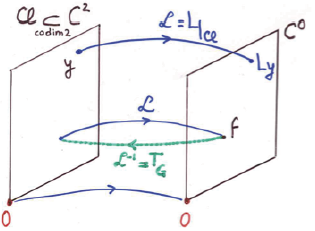
\includegraphics[scale=0.3]{image18.png}
\captionof{figure}{Existence}
\end{wrapfigure}


Si $Ly=0$ n'admet que la solution triviale dans $Cl$
\begin{enumerate}
\item $L|_{Cl}$ admet une et une seule fonction de Green $G(x;\xi)$
\item Si $f\in C^0([a,b],\mathbb{R})$, alors la solution du problème non-homogène $Ly = f$ admet pour seule solution la fonction $y$ dans $Cl$ définie par
\begin{equation}
y(x) = \int_a^b G(x,\xi)f(\xi)d\xi
\end{equation}
\end{enumerate}}

\subsection{Existence et unicité de la fonction de Green}
\proposition{Si le problème homogène n'admet que la solution triviale, alors il existe une et une seule fonction de Green associée à $\mathcal{L}$ sur $[a,b]$.}\ \\

\setcounter{subsection}{5}
\subsection{Résolution du PnH grâce à Green}
Si le problème homogène associé $Ly = 0$ a une seule solution dans $C^n([a,b]) \cap Cl$, alors le problème non homogène $Ly = f$ a une et une seule solution dans $C^n([a,b]) \cap Cl$, à savoir la fonction $y$ donné par
\begin{equation}
y(x) := \int_a^b f(\xi)G(x;\xi)d\xi
\end{equation}
\begin{proof}
Longue et fastidieuse, cf. syllabus page 56.
\end{proof}

\newpage
\subsection{$G$ calculée pour Sturm-Liouville}
Soit $L(y) := -(py')' + qy$ un opérateur régulier et $p$ ne s'annule pas sur $[a,b]$. Considérons les (CLH)
\begin{equation}
\left\{\begin{array}{ll}
\alpha_0y(a) + \alpha_1y'(a) &=0\\
\beta_0y(b) + \beta_1y'(b) &=0
\end{array}\right.\ \ \ \ \ (\alpha_0,\alpha_1- \neq (\beta_0,\beta_1)
\end{equation}
Considérons
\begin{itemize}
\item $y_a$ := la solution du problème de Cauchy : $Ly_a = 0,y_a(a) = \alpha_1, y'_a(a) = -\alpha_0$
\item $y_a$ := la solution du problème de Cauchy : $Ly_b = 0,y_b(b) = \beta_1, y'_b(b) = -\beta_0$
\end{itemize}
\textbf{Si} le problème n'admet \textbf{que} la solution triviale, alors $y_a$ et $y_b$ sont linéairement indépendants et la fonction de Green associée à $L|_{Cl}$ est la fonction symétrique
\begin{equation}
G(x;\xi) = \left\{\begin{array}{ll}
\dfrac{-1}{pW(y_a,y_b)}y_a(x)y_b(\xi) &\ si\ x\leq \xi\\
\dfrac{-1}{pW(y_a,y_b)}y_a(\xi)y_b(x) &\ si\ x\geq \xi
\end{array}\right.
\end{equation}
\begin{proof}
A étudier ? Page 57-58.
\end{proof}

\subsection*{Une histoire !}
\begin{wrapfigure}[14]{r}{3cm}
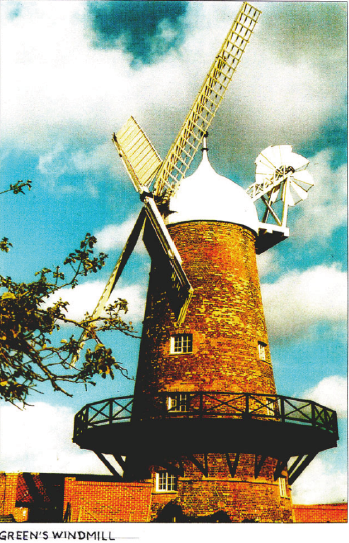
\includegraphics[scale=0.3]{image19.png}
\captionof{figure}{Moulin de Green}
\end{wrapfigure}
Comme on a bien travaillé, voici une petite histoire sur la vie de Mr. Green et son fameux moulin\footnote{Source : Wikipédia} !\\
George Green (juillet 1793 - 31 mai 1841) est un physicien britannique.L'histoire de la vie de George Green a ceci d'exceptionnel qu'il était presque totalement autodidacte. Il est né et a vécu la plus grande partie de sa vie dans la ville anglaise de Sneinton, qui fait aujourd'hui partie intégrante de la ville de Nottingham. Son père (également prénommé George) était un boulanger qui avait construit et possédait un moulin à vent utilisé pour moudre le grain. Le jeune George Green n'a passé qu'un an environ à l'école, entre 8 et 9 ans.\\
Le moulin à vent des Green.
Au cours de sa vie adulte, George Green a travaillé dans le moulin de son père, en héritant à la mort de celui-ci en 1829. Il commença à étudier les mathématiques à un moment indéterminé de sa vie. La ville de Nottingham ayant à cette époque une vie intellectuelle restreinte, la manière dont il obtint des informations sur les développements de cette science n'est pas claire pour les historiens. Une seule personne possédant une instruction reconnue en mathématiques, John Toplis, aurait vécu à Nottingham à cette époque. Lorsque Green publia son essai en 1828, il fut édité sur la base d'une souscription de 51 personnes, dont la plupart faisaient partie de ses amis et ne pouvaient probablement pas comprendre ses travaux. Le mathématicien Edward Bromhead en acheta une copie et encouragea Green à poursuivre son travail en mathématiques. Ne croyant pas l'offre sincère, Green ne prit pas contact avec lui avant 2 ans.\\
Green finit toutefois par contacter Bromhead, qui lui permit d'entrer à l'université de Cambridge. Il l'intégra comme étudiant en 1833 à l'âge de 40 ans. Sa carrière fut excellente, et une fois son diplôme obtenu en 1837, il demeura à la faculté de "Gonville et Caius College". Il écrivit des publications dans le domaine de l'optique, de l'acoustique et de l'hydrodynamique. Cependant, il tomba gravement malade en 1840 et rentra à Nottingham, où il mourut l'année suivante. En 1986, son moulin a été restauré. Il sert maintenant à la fois d'exemple de fonctionnement d'un moulin du xixe siècle et de musée consacré à sa vie et à son travail.


\setcounter{chapter}{21}
\chapter{Classification des EDP quasi-linéaires du second ordre}
\section{Les solutions d'une EDPL}
\subsection{Introduction}
Une équations aux dérivées partielles (EDP) du second ordre en une fonction inconnue $u$ de 2 variables $x$ et $y$ est une expression du type
\begin{equation}
F\left( x,y,u,\frac{\partial u}{\partial x},\frac{\partial u}{\partial y}, \frac{\partial^2 u}{\partial x^2}, \frac{\partial^2 u}{\partial x\partial y}, \frac{\partial^2 u}{\partial y^2}\right)
\end{equation}
non triviale en $\left(\frac{\partial^2 u}{\partial x^2}, \frac{\partial^2 u}{\partial x\partial y}, \frac{\partial^2 u}{\partial y^2}\right)$.Pour alléger l'écriture, on écrit souvent $u_{xx}$ pour $\dfrac{\partial^2u}{\partial x^2}$, $u_{xy}$ pour $\dfrac{\partial^2u}{\partial x \partial y}, \dots$ \\
Lors que la variable est le temps ($t$), on parlera d'équation d'\textit{évolution}.


\subsection{Linéarité}
Une EDP est \textbf{linéaire} ssi elle peut être écrite sous la forme 
\begin{equation}
Lu = g
\end{equation}
où $g$ est fonction des variables indépendantes et $L$ un opérateur différentiel linéaire.\\
Toute combilis de $L$ est aussi linéaire : les dérivées partielles, mixtes, ... seront également linéaires : l'ensemble des solution de l'EDPH est un espace vectoriel.\\
La \textbf{forme générale d'une EDP linéaire du second ordre} où l'inconnue $y$ est fonction de $x$ et $y$ :
\begin{equation}
a\frac{\partial^2u}{\partial x^2} + 2b\frac{\partial^2u}{\partial x\partial y} + c\frac{\partial^2u}{\partial y^2} + d\frac{\partial u}{\partial x} + e\frac{\partial u}{\partial y} + fu = g
\end{equation}
où $a,b,c,d,e,f,g$ sont des fonctions de $(x,y)$ (fonction cubique, quadratique, exponentielle, bref salade tout).\\On définit la notion d'EDP \textbf{quasi-linéaire}\footnote{Car terme en $u$ non linéaire.} : 
\begin{equation}
a\frac{\partial^2u}{\partial x^2} + 2b\frac{\partial^2u}{\partial x\partial y} + c\frac{\partial^2u}{\partial y^2} = f\left(x,y,u,\frac{\partial u}{\partial x}, \frac{\partial u}{\partial y}\right)
\end{equation}


\setcounter{subsection}{3}
\subsection{Quel problème poser ?}
\subsubsection{EDP et ED : "analogie"}
On va ici chercher à généraliser les propriétés obtenues pour les problèmes de Cauchy dans une ED (existence et unicité). Tentons de faire l'analogie en partant d'une \textbf{EDL du second ordre }:
\begin{equation}
u'' = 0
\end{equation}
La solution générale $u(x) = ax+b$ (EV de dimension 2) dépend de deux constantes arbitraire. En imposant une \textbf{CI} :$\left\{\begin{array}{ll}
u(0) &= u_0\\
u'(0) &= u_1
\end{array}\right.$. Cela revient à imposer que le graphe de $u$ passe par le point $(0,u_0)$ et que sa pente en ce point soit $u_1$ : le problème admet \textbf{une et une seule} solution. Inspirons nous de ceci pour aborder d'\textbf{EDP} :
\begin{equation}
\frac{\partial^2u}{\partial x^2} = 0
\end{equation}
Par double intégration, on trouve la solution générale : $u(x,y) = a(y)x + b(y)$ (EV de dimension infinie) ou cette fois $a$ et $b$ sont deux \textbf{fonctions arbitraires}  suffisamment dérivable. En s'inspirant du problème de Cauchy pour l'ED :
\begin{equation}
\left\{\begin{array}{ll}
u(0,y) &= y_0(y)\\
\frac{\partial y}{\partial x}(0,y) &= u_1(y)
\end{array}\right.
\end{equation}
$\rightarrow$ Notre problème n'admet qu'une et une seule solution.  L'interprétation graphique est :
\begin{enumerate}
\item La première partie impose que la graphe de $u$ s'appuie sur la courbe $C \equiv \left\{\begin{array}{l}
u = u_0(y)\\
x = 0
\end{array}\right.$
\item La deuxième partie impose que la pente de la tangente de chacune des sections de la surface du gph $u$ par des plan $y=y^*=c^{ste}$. Si l'on prolonge tous ces segments tangents, on obtiendrait le graphe de $u$, une surface réglée.
\end{enumerate}
Ce problème est \textbf{bien posé} en ce sens qu'il n'admet qu'une unique solution.

\subsubsection{Permutation $x$ et $y$}
En effectuant cette permutation dans les conditions initiales, celles-ci restent toujours "du même type" que la précédente et donc intrinsèquement bonne...
\begin{equation}
\left\{\begin{array}{ll}
u(x,0) &= f(x)\\
\frac{\partial u}{\partial y}(x,0) &= g(x)
\end{array}\right.
\end{equation}
... mais pour cette EDP, c'était ce qu'il ne fallait pas faire : la résolution du problème est impossible sauf si $f$ et $g$ sont de degré $\leq 1$ et même si c'est le cas on trouverait une infinité de solution car $a$ et $b$ ne seraient pas  univoquement déterminée : le problème est \textbf{mal posé}\footnote{Il serait bien posé dans le cas ou l'on aurait pour EDP : $\frac{\partial^2y}{\partial y^2} =0$.}.
\subsubsection{Condition intrinsèquement mauvaise}
Le problème de Cauchy :
\begin{equation}
\left\{\begin{array}{ll}
u(x,0) &= f(x)\\
\frac{\partial u}{\partial x}(x,0) &= g(x)
\end{array}\right.
\end{equation}
impose que $g(x) = f'(x)$ ce qui peut être contradictoire ou au mieux redondant.\\

Le type de condition dépend de l'ordre de L'EDP mais aussi de l'EDP ! Pour s'y retrouver on défini les \textit{courbes caractéristiques}, c'est à dire les courbes ou il ne faut \textbf{pas} imposer de CI. En gros :
\begin{itemize}
\item Ne jamais donner sur une droite : $u$ et sa dérivée dans cette direction
\item Ne jamais donner sur une droite : $u$ et sa dérivée le long de cette courbe
\end{itemize}


\section{Problème de Cauchy et courbes caractéristiques}
\setcounter{section}{2} 
\subsection{Problème de Cauchy pour les EDM QL d'ordre 2}
\begin{wrapfigure}[10]{r}{5cm}
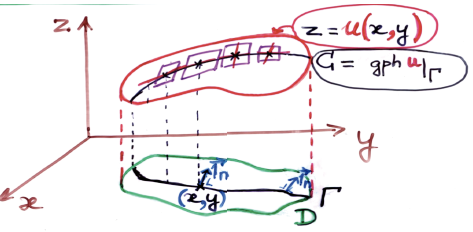
\includegraphics[scale=0.5]{image20.png}
\captionof{figure}{Paramétrisation $\Gamma$}
\end{wrapfigure}
Soit l'EDP quasi-linéaire
\begin{equation}
a\frac{\partial^2u}{\partial x^2} + 2b\frac{\partial^2u}{\partial x\partial y} + c\frac{\partial^2u}{\partial y^2} = f\left(x,y,u,\frac{\partial u}{\partial x}, \frac{\partial u}{\partial y}\right)
\end{equation}
Soit $\Gamma$ une courbe régulière dans $D$ (un ouvert de $\mathbb{R}^2$) de paramétrisation $\vec{\gamma} : I \rightarrow \mathbb{R}^2 : s \rightarrow \left(\begin{array}{c}
x(s)\\
y(s)
\end{array}\right)$. Il apparaît naturel de se donner comme condition les valeurs de $u$ et $\vec{\nabla}u$ sur $\Gamma$. On remarque qu'il suffit de se donner $u$ et la dérivée normale $\frac{\partial u}{\partial n}$ de $u$ sur $\Gamma$.
\begin{equation}
\left.\frac{\partial u}{\partial x}\right|_{\vec{\gamma}(s)}x'|_s +\left.\frac{\partial u}{\partial y}\right|_{\vec{\gamma}(s)}y'|_s = \frac{d}{ds}\underbrace{u(x(s),y(s))}_{\text{fct connue}}
\end{equation}

\subsection{Courbes caractéristiques d'une EDP}
Afin de trouver une solution, nous allons utiliser Taylor : il faut avant tout calculer les différentes dérivées. Comme on a $u|_\Gamma, \left.\frac{\partial u}{\partial x}\right|_\Gamma$ et $\left.\frac{\partial u}{\partial y}\right|_\Gamma$, on a\footnote{Les lignes 2 et 3 sont les dérivées de la première ligne par rapport à $x$ et $y$.} :
\begin{equation}
\left\{\begin{array}{ll}
a|_{\vec{\gamma}(s)} + 2b|_{\vec{\gamma}(s)}\left.\dfrac{\partial^2 u}{\partial x \partial y}\right|_{\vec{\gamma}(s)} + c|_{\vec{\gamma}(s)}\left.\dfrac{\partial^2u}{\partial y^2}\right|_{\vec{\gamma}(s)} &= f(\vec{\gamma}(s), u|_{\vec{\gamma}(s)}, \vec \nabla u|_{\vec{\gamma}(s)})\\
\left.\dfrac{dx}{ds}\right|_{s}\left.\dfrac{\partial^2u}{\partial x^2}\right|_{\vec{\gamma}(s)} + \left.\dfrac{dy}{ds}\right|_{s}\left.\dfrac{\partial^2u}{\partial x\partial y}\right|_{\vec{\gamma}(s)} &= \dfrac{d}{ds}\left(\left.\dfrac{\partial u}{\partial x}\right|_{\vec{\gamma}(s)}\right)\\
\left.\dfrac{dx}{ds}\right|_{s}\left.\dfrac{\partial^2u}{\partial x\partial y}\right|_{\vec{\gamma}(s)} + \left.\dfrac{dy}{ds}\right|_{s}\left.\dfrac{\partial^2u}{\partial y^2}\right|_{\vec{\gamma}(s)} &= \dfrac{d}{ds}\left(\left.\dfrac{\partial u}{\partial y}\right|_{\vec{\gamma}(s)}\right)
\end{array}\right.
\end{equation}
Il s'agit d'un système algébrique linéaire de déterminant  :
\begin{equation}
\left|\begin{array}{ccc}
a & 2b & c\\
\dfrac{dx}{ds} & \dfrac{dy}{ds} & 0\\
0 & \dfrac{dx}{ds} & \dfrac{dy}{ds}
\end{array}\right| = a|_{(x(s),y(s))} \left(\dfrac{dy}{ds}\right)^2 - 2b|_{(x(s),y(s))} \dfrac{dx}{ds}\dfrac{dy}{ds} + c|_{(x(s),y(s))}\left(\dfrac{dx}{ds}\right)^2
\end{equation}
En tout point $(x(s),y(s)) \in \Gamma$ où ce déterminant $\neq 0$, les dérivées secondes de $u$ sont \textbf{univoquement déterminée}.\\
Le système sera bien posé si
\begin{equation}
 a|_{(x(s),y(s))} \left(\dfrac{dy}{ds}\right)^2 - 2b|_{(x(s),y(s))} \dfrac{dx}{ds}\dfrac{dy}{ds} + c|_{(x(s),y(s))}\left(\dfrac{dx}{ds}\right)^2 \neq 0
\end{equation}
C'est à dire si la "pente de $\Gamma$ en $(x,y)$ dy/dx \textbf{n'est pas} (car il faut $\neq 0)$ solution de\footnote{On divise tout par dx/ds}
\begin{equation}
a\left(\dfrac{dy}{dx}\right)^2 - 2b\dfrac{dy}{dx} + c = 0
\end{equation}
C'est à dire si :
\begin{equation}
\dfrac{dy}{dx} \neq \dfrac{b\pm \sqrt{b^2-ac}}{a}
\end{equation}
\textbf{Inversement}\footnote{Dans le sens : les dérivés secondes ne seront pas univoquement déterminée.}, les courbes caractéristiques de l'EDP sont les courbes intégrales de l'ED des caractéristiques :
\begin{equation}
a(x,y)dy^2 - 2b(x,y)dxdy + c(x,y)dx^2 = 0
\end{equation}
Les directions caractéristiques sont les directions de $(x,y)$ solution de cet équation.\\Par définition, que les pentes caractéristiques sont :
\begin{equation}
\omega^\pm = \dfrac{dy}{dx} = \dfrac{b\pm \sqrt{b^2-ac}}{a}
\end{equation}
On aura, en fonction du signe du discriminant :
\begin{itemize}
\item Deux direction caractéristiques \textit{hyperboliques} si $b^2-ac > 0$
\item Une direction caractéristique \textit{parabolique} si $b^2-ac = 0$
\item Pas de caractéristique \textit{elliptique} si Deux direction caractéristiques si $b^2-ac < 0$
\end{itemize}

\subsection{Résolution locale à la Cauchy - Kovaleskaya}
Si l'on prend une condition de Cauchy sur $\Gamma$, deux cas sont possibles :
\begin{enumerate}
\item Si $\Gamma$ est caractéristique, c'est la cata :(
\item Si ce ne l'est pas (et que ce n'est pas tangent à une caractéristique) alors, en tout point de $\Gamma$, toutes les dérivées secondes de $u$ sont univoquement déterminées.
\end{enumerate}
De même, les dérivées $3^e$ de $u$ le sont aussi, $\dots$\\

\theor{\textsc{Cauchy-Kovaleyskaya}\\
Pour une EDP + CI sur $\Gamma$ (non-caractéristique) est déterminée univoquement par le développement de Taylor de $u$ en tout point de $\Gamma$ d'où l'uniticité locale d'une éventuelle solution analytique du problème de Cauchy et l'existence si on a les bonnes convergences.} \ \\
Autrement dit, si $\Gamma$ n'est pas une courbe caractéristique alors de telle CI déterminent univoquement le développement de Taylor : si celui-ci converge il s'agit d'une solution qui sera unique.

\newpage
\section{Classification des EDPQLcc}
Considérons les EDP du type\footnote{$a,b$ et $c$ sont évalués en $(x,y)$.} :
\begin{equation}
\underbrace{\frac{\partial^2u}{\partial x^2} + 2b\frac{\partial^2u}{\partial x\partial y} + c\frac{\partial^2u}{\partial y^2}}_{\text{Partie principale, L(u) :=}} = f\left(x,y,u,\frac{\partial u}{\partial x}, \frac{\partial u}{\partial y}\right)
\end{equation}

\subsection{Changement de variable linéaire sur $\mathbb{R}^2$ pour EDP QL à coefficients constants}
L'opérateur $L$ défini ci-dessus peut être écrit (\textbf{où} cette fois $a,2b,c$ sont constant!!):
\begin{equation}
L(u) : (\partial_x\ \partial_y)\left(\begin{array}{cc}
a & b\\
b & c
\end{array}\right)\left(\begin{array}{c}
\partial_x\\
\partial_y
\end{array}\right)u
\end{equation}
Comme $L$ est linéaire, on peut faire un changement de coordonnée linéaire pour passer de $(x,y)$ à $(\xi,n)$ :
\begin{equation}
\left(\begin{array}{c}
\xi\\
\eta
\end{array}\right) := \left(\begin{array}{cc}
p_{11} & p_{12}\\
p_{21} & p_{22}
\end{array}\right)\left(\begin{array}{c}
x\\
y
\end{array}\right) = P\left(\begin{array}{c}
x\\
y
\end{array}\right)
\end{equation}
En effectuant les dérivées en cascades, on obtient :
\begin{equation}
(\partial_x\ \partial_y)\left(\begin{array}{cc}
a & b\\
b & c
\end{array}\right)\left(\begin{array}{c}
\partial_x\\
\partial_y
\end{array}\right)\ "="\  (\partial_\xi\ \partial_\eta)P\left(\begin{array}{cc}
a & b\\
b & c
\end{array}\right)P^t\left(\begin{array}{c}
\partial_\xi\\
\partial_\eta
\end{array}\right)
\end{equation}
L'EDP en $u (x,y) \mapsto u(x,y)$ qui s'écrivait initialement : 
\begin{equation}
(\partial_x\ \partial_y)\left(\begin{array}{cc}
a & b\\
b & c
\end{array}\right)\left(\begin{array}{c}
\partial_x\\
\partial_y
\end{array}\right)u = f\left(x,y,u,\frac{\partial u}{\partial x}, \frac{\partial u}{\partial y}\right)
\end{equation}
se transforme en l'EDP en $\tilde{u}:(\xi,\eta) \mapsto \tilde{u}(\xi,\eta)$:
\begin{equation}
(\partial_\xi\ \partial_\eta)\ \underbrace{P\left(\begin{array}{cc}
a & b\\
b & c
\end{array}\right)P^t}_{:= D}\left(\begin{array}{c}
\partial_\xi\\
\partial_\eta
\end{array}\right)\tilde{u} = g\left(\xi,\eta,\tilde{u},\frac{\partial \tilde{u}}{\partial x}, \frac{\partial \tilde{u}}{\partial y}\right)
\end{equation}
On espère bien évidemment que la matrice $D$ (matrice des coefficient de la principale) soit plus simple que la matrice 'initiale'.

\subsection{Forme canonique diagonale sur $\mathbb{R}^2$}
L'idée est de choisir $P$ telle que $PAP^t =: D$ soit \textit{diagonale}. Si on se restreint aux changements de coordonnés \textbf{isométriques} alors les coefficients de $D$ sont les valeurs propres $\lambda_1$ et $\lambda_2$ de $A$ :
\begin{equation}
A = \left(\begin{array}{cc}
a & b\\
b & c
\end{array}\right) \mapsto \left(\begin{array}{cc}
\lambda_1 & 0\\
0 & \lambda_2
\end{array}\right) = D
\end{equation}
On retrouve alors :
\begin{itemize}
\item $\lambda_1.\lambda_2 < 0 \Leftrightarrow b^2-ac > 0 \Leftrightarrow$ EDP \textit{hyperbolique}
\item $\lambda_1.\lambda_2 = 0 \Leftrightarrow b^2-ac = 0 \Leftrightarrow$ EDP \textit{parabolique}
\item $\lambda_1.\lambda_2 > 0 \Leftrightarrow b^2-ac < 0 \Leftrightarrow$ EDP \textit{elliptique}
\end{itemize}

\setcounter{subsection}{3}
\subsection{Forme canonique "factorisée" des EDPQL}
Soit l'EDP QL : 
\begin{equation}
(\partial^2_x + 2b\partial_x\partial_y + c \partial_u^2)u = f
\end{equation}
L'idée est de factoriser l'opérateur linéaire du premier membre sous forme composée de deux opérateurs linéaires du premier ordre comme ceci :
\begin{equation}
(\partial_x - \omega^+ \partial_y)(\partial_x - \omega^- \partial_y)
\end{equation}
En distribuant\footnote{Notons que $\omega$ n'est pas forcément constant.}, on trouve
\begin{equation}
(\partial_x^2 - \partial_x\omega^-\partial_y - \omega^+\partial_y\partial_x + \omega^+\partial_y\omega^-\partial_y)
\end{equation}
Après mise en évidence :
\begin{equation}
\underbrace{(\partial^2_x -(\omega^-+\omega^+)\partial_x\partial_y + \omega^+\omega^-\partial_y^2)}_{\text{2nd ordre (partie princ.)}} - \underbrace{\left(\frac{\partial \omega^-}{\partial x}-\omega^+\frac{\partial \omega^-}{\partial_y}\right)\partial_y}_{\text{1er ordre}}
\end{equation}
En identifiant l'expression du second ordre avec notre EDL QL ci-dessus :
\begin{equation}
(\partial_x^2 + \frac{2b}{a}\partial_x\partial_y + \frac{c}{a}\partial_y^2)
\end{equation}
Par identification, $\omega^-+\omega^+ = -\frac{2b}{a}$ et que $\omega^-\omega^+ = \frac{c}{a}$.\\
Les racines de $a\omega^2 +2b\omega + c = 0$ sont donnée par:
\begin{equation}
\omega^\pm : \dfrac{-b\pm \sqrt{b^2-ac}}{a}
\end{equation}
On retrouve une fois de plus\footnote{Notons que le dernier terme (du 1er ordre) n'apparaît pas si $a,b,c$ sont des constantes.} : 
\begin{itemize}
\item Si $\omega^\pm$ sont deux réels différent : EDP \textit{hyperbolique}
\item Si $\omega^\pm$ sont deux complexes conjugués: EDP \textit{elliptique}
\item Si $\omega^+=\omega^-$ est un réel : EDP \textit{parabolique}
\end{itemize}

\subsection{Forme canonique hyperbolique "factorisée"}
Au premier ordre près, on peut dire que
\begin{equation}
(\partial_x - \omega^+ \partial_y)(\partial_x - \omega^- \partial_y) = \partial_x^2 + \frac{2b}{a}\partial_x\partial_y + \frac{c}{a}\partial_y^2
\end{equation}
ou encore, en inversant le signe sachant que, grâce à l'ED des caractéristiques $\frac{dy}{dx} = -\omega^\pm$ :
\begin{equation}
(\partial_x + \omega^+ \partial_y)(\partial_x + \omega^- \partial_y) = \partial_y^2 - \frac{2b}{a}\partial_x\partial_y + \frac{c}{a}\partial_x^2
\end{equation}

\subsubsection{Supposons l'EDP hyperbolique}
Si $a,b,c$ sont constant, $\frac{dy}{dx} = c^{te}$. Les droites caractéristiques sont donnée par (en partant de l'ED des caract.):
\begin{equation}
\left\{\begin{array}{ll}
y+\omega^+x &= c^{te}\\
y+\omega^-x &= c^{te}
\end{array}\right.
\end{equation}
Ceci étant "remarqué", introduisons le changement de variable linéaire suivant :
\begin{equation}
\left\{\begin{array}{ll}
\xi &= y +\omega^+x\\
\eta &= y +\omega^-x
\end{array}\right.
\end{equation}
Les droits caractéristiques $\equiv$ :
\begin{equation}
\left\{\begin{array}{ll}
\xi(x,y) &= c^{te}\\
\eta(x,y) &= c^{te}
\end{array}\right.
\end{equation}
\retenir{Dans les variables $(\xi,eta)$, l'EDP 
\begin{equation}
au_{xx} + 2bu_{xy} + cu_{yy} = f(x,y,u,\dots)
\end{equation}
devient
\begin{equation}
\tilde{u}_{\xi\eta} = g(\xi,\eta,\tilde{u}, \tilde{u}_\xi, \tilde{u}_\eta)
\end{equation}}\ \\

Ce qui est nettement plus sympathique à résoudre ('démo' en exercice)!



\chapter{EDP des ondes}
\section{Modèles expérimentaux}
\subsection{La corde vibrante}
L'équation de la corde vibrante est un grand classique du cours de \textit{Physique Générale} :
\begin{equation}
\frac{\partial^2 u}{\partial t^2} = c^2\frac{\partial u^2}{\partial x^2}\ \ \ \ \ \ \ \forall x,t
\end{equation}
où le premier terme désigne l'accélération verticale et le second la concavité de la forme de la corde. Cette dernière sera forte vers le haut (bas) si l'accélération est forte vers le haut (bas).


\section{EDP des ondes dans $\mathbb{R}$}
\subsection{Droites caractéristiques et S.G.}
Reprenons l'équation d'onde (23.1) : l'EDO des caractéristiques vaut $\frac{dx}{dt} = \pm c$, impliquant des droites caractéristiques de la forme $x \pm ct = cste$. Posons :
\begin{equation}
\left\{\begin{array}{l}
\xi := x + ct\\
\eta := x - ct
\end{array}\right.\ \ \Rightarrow \left(\begin{array}{c}
\xi\\
\eta
\end{array}\right) = \left(\begin{array}{cc}
1 & c\\
1 & -c
\end{array}\right)\left(\begin{array}{c}
x\\
t
\end{array}\right)
\end{equation}
d'où (\textbf{???}) :
\begin{equation}
\left(\begin{array}{c}
\partial x\\
\partial y
\end{array}\right) "=" \left(\begin{array}{cc}
1 & 1\\
c & -c
\end{array}\right)\left(\begin{array}{c}
\partial\xi\\
\partial\eta
\end{array}\right)
\end{equation}
Après application du changement de variable, notre EDP devient :
\begin{equation}
4c^2 \dfrac{\partial^2 \tilde{u}}{\partial\xi\partial\eta} = 0
\end{equation}
La résolution de cette équation s'obtient facilement :
\begin{equation}
\dfrac{\partial}{\partial\xi}\left(\begin{array}{c}
\dfrac{\partial\tilde{u}}{\partial \eta}
\end{array}\right) = 0 \Rightarrow \dfrac{\partial\tilde{u}}{\partial\eta} = h(\eta) \rightarrow \tilde{u} = \underbrace{\int h(\eta)d\eta}_{g(\eta)} + f(\xi)
\end{equation}
Après subtitution, on trouve la solution générale :
\begin{equation}
u(x,t) = f(x+ct) + g(x-ct)
\end{equation}
où $f,g \in C^2$ sont des fonctions arbitraires. Cela s'interprète comme la superposition d'une onde $f$ qui se propage à vitesse $-c$ et une onde $g$ qui se propage à vitesse $c$.

\subsection{C.I. de Cauchy et solution de d'Alembert}
Considérons une condition initiale (position et vitesse) bien posée (dérivée par rapport à la perpendiculaire à l'instant initial) :
\begin{equation}
(C.I.)\ \left\{\begin{array}{ll}
u(x,0) &= \phi(x)\\
\frac{\partial u}{\partial t}(x,0) &= \psi(x)
\end{array}\right.
\end{equation}
On connait la S.G., il faut trouver $u$ compte-tenu de la C.I. :
\begin{equation}
\left\{\begin{array}{ll}
\phi(x) &= \varphi(x)\\
\psi(x) &= c(f'(x)-g'(x))
\end{array}\right.\ \ \ \Rightarrow 
\end{equation}
Dérivons la première équation pour  travailler avec deux équations différentielle et division la deuxième par $c$ :
\begin{equation}
\left\{\begin{array}{ll}
\phi'(x) &= \varphi(x)\\
\frac{\psi(x)}{c} &= c(f'(x)-g'(x))
\end{array}\right.
\end{equation}
Après résolution du système, on trouve :
\begin{equation}
\left\{\begin{array}{ll}
f'(x) &= \frac{1}{2}\left(\phi'(x) + \frac{\psi(x)}{c}\right)\\
g'(x) &= \frac{1}{2}\left(\phi'(x) - \frac{\psi(x)}{c}\right)
\end{array}\right.
\end{equation}
Après intégration :
\begin{equation}
\left\{\begin{array}{ll}
f(x) &= \frac{1}{2}\phi(x) + \frac{1}{2c}\int_0^x \psi + A\\
g(x) &= \frac{1}{2}\phi(x) - \frac{1}{2c}\int_0^x \psi + B
\end{array}\right.
\end{equation}
En effectuant $f(x) + g(x)$, il faut retrouver $\phi(x)$ (pour respecter la C.I.), ce qui n'est possible que si $(A+B) = 0$.\\
On trouve alors comme solution générale associée au problème de Cauchy :\\

\retenir{\textsc{Formule de d'Alembert}
\begin{equation}
u(x,t) = \frac{1}{2}(\phi(x+ct) + \phi(x-ct)) + \frac{1}{2c}\int_{x-ct}^{x+ct} \psi
\end{equation}}\ \\
On notera que si $\phi \in C^2, \psi \in C^1$, alors $u\in C^2$ est solution de l'EDP satisfaisant au C.I. (pour vérifier, remplacer !). En faisant le raisonnement précédent, on arrive bien à l'existence et l'unicité de la solution.

\subsection{Dessin animé de la corde pincée}
Simple illustration. Cf. page 8/slide 12.

\subsection{Dessin animé du coup de marteau}
Simple illustration. Cf. page 9/slide 14.

\subsection{Principe de causalité}
Bien lire les page 10-12, c'est assez littéraire ! Retenons néanmoins :\\

\corollaire{Si les C.I. sont à support compact, alors la solution de l'EDP des ondes homogène est, à tout instant, à support compact.\\
On verra (spoil) que ceci sera également d'application pour l'EDP non-homogène si le terme source $F(x,t)$ est aussi à support compact (c-à-d nul partout sauf sur un compact).}

\subsection{Loi de conservation de l'énergie}
Encore très descriptif, mais sympa à lire : page 13.


\section{EDP des ondes non homogènes}
\subsection{Superposition des solutions de problèmes linéaires complémentaires}
Considérons cette fois une équation d'onde comportant un terme forçant, c'est-à-dire non-homogène :
\begin{equation}
\dfrac{\partial^2u}{\partial t^2} - c^2\dfrac{\partial^2u}{\partial x^2} = F(x,t)
\end{equation}
Si ce problème venait à être trop compliqué, on peut le décomposer en deux problèmes complémentaires :
\begin{enumerate}
\item EDP non homogène, mais avec des CI homogène : $u_F$
\item EDP homogène, mais avec des CI non homogène : $u_{\varphi,\psi}$
\end{enumerate}
\theor{\textsc{Principe de superposition}\\
\begin{equation}
u = u_F + u_{\varphi,\psi}
\end{equation}}
\begin{proof}
\ \\
Par linéarité du problème (EDP + CI) $\Rightarrow u_F + u_{\varphi,\psi}$ est solution. Notons également que c'est \textbf{la seule} solution (23.3.3 : unicité). On peut donc écrire $u = u_F + u_{\varphi,\psi}$.
\end{proof}

\subsection{Méthode de Lagrange pour les EDL}
Cette section n'est qu'un mignon petit rappel. La fonction de Lagrange est utilisée pour résoudre les EDLnH à partir de la solution de l'EDLH avec des CI non homogène. Pour l'opérateur différentiel :
\begin{equation}
L(y) = a_0 y^{(p)} + \dots + a_{p-1}y' + a_p y
\end{equation}
Nous avions par définition de la fonction de Lagrange :
\begin{equation}
l(t;\tau) = y(t;\tau,(0,\dots, \frac{1}{a_0}),0)
\end{equation}
La solution de ($Ly = b$ + CIH) est alors donnée par :
\begin{equation}
y(t) = \int_{t_0}^t l(t,\tau)b(\tau)d\tau
\end{equation}



\subsection{Principe de Duhamel pour EDP}
Il s'agit en quelque sorte d'une généralisation de la méthode de Lagrange pour les EDP. Cette méthode permet de déluire la solution du problème (EDPnH + CIH) de celle du problème (EDPH + CInH).\\
Afin d'illustrer la méthode, considérons le problème de vibration forcée d'un corde illimitée :
\begin{equation}
\left\{\begin{array}{lr}
u_{tt} - c^2u_{xx} = f\\
u(x,0) = \varphi(x)&\ \ \ \ \ \ \ \ \ \ \ \forall x\in \mathbb{R}, t\in \mathbb{R}^+\\
u_t(x,p) = \psi(x) & \forall x \in \mathbb{R}
\end{array}\right.
\end{equation}
Appliquons le principe de superposition : résolvons le problème associé où le CI sont homogènes :
\begin{equation}
(P)\ \left\{\begin{array}{llr}
(EDPnH) &: u_{tt} - c^2u_{xx} = f&\ \ \ \ sur\ \mathbb{R}\times\mathbb{R}^+\\
(CIH) &: u(x,0) = 0, u_t(x,0) = 0 &\ \ \ \forall x \in \mathbb{R}
\end{array}\right.
\end{equation}
Duhamel associé à $(P)$ une infinité de problème $(P_\tau)$ non forcés mais à CInH ou l'instant initial varie dans le temps :
\begin{equation}
(P_\tau)\ \left\{\begin{array}{ll}
(EDPH) &: u_{tt} - c^2u_{xx} = 0\\
(CI_\tau) &: v(x,\tau) = 0, v_t(x,\tau) = f(x,\tau)
\end{array}\right.
\end{equation}
Notons $v(x,t;\tau)$ la solution du problème $(P_\tau)$. On peut imaginer que \textit{la solution $u(x,t)$ au problème $(P)$ est la \textbf{superposition des réponses $v(x,t;\tau)$} aux impulsions imposées aux instants $\tau$ compris entre le véritable instant initial 0 et l'instant $t$.}\ \\

\theor{Principe de Duhamel\\
La fonction 
\begin{equation}
u(x,t) = \int_0^t v(x,t,\tau) d\tau
\end{equation}
est solution du problème $(P)$.}\ \\
La solution $u(x,t)$ s'obitent en intégrant toutes les contributions des "CI élémentaires".

\begin{proof}
Assez longue mais pas très compliquée, cf. syllabus page 16' et slides 25-26.
\end{proof}


\subsection{Solution calculée grâce à Duhamel}
Appliquons ce principe aux vibrations forcées d'une corde infinie. Utilisons la solution d'Alembert qui dit (pour un temps initial $\tau$) :
\begin{equation}
v(x,t;\tau) = \dfrac{1}{2c}\int_{x-c(t-\tau)}^{x+c(t-\tau)} f(s,\tau)\ ds
\end{equation}
Par Duhamel, on en conclut :
\begin{equation}
u(x,t) = \dfrac{1}{2c} \int_0^t\left(\int_{x-c(t-\tau)}^{x+c(t-\tau)} f(s,\tau)\ ds\right)d\tau
\end{equation}
Par Fubini, on trouve finalement que :
\begin{equation}
u(x,t) = \dfrac{1}{2c}\iint_{\Delta(x,y)} f(s,\tau)\ ds\ d\tau
\end{equation}



\subsection{Problème bien posé}
Un probl!me est "bien posé" lorsqu'il respecte "la trinité" selon Hadamard, c'est à dire l'\textit{unicité, l'existance} et la \textit{stabilité}. Considérons le problème de Cauchy pour une corde illimité :
\begin{equation}
\left\{\begin{array}{ll}
\frac{\partial^2u}{\partial t^2} - c^2\frac{\partial^2u}{\partial x^2} &= f(t)\\
u(x,0) &= \varphi(x)\\
\frac{\partial u}{\partial t}(x,0) &= \psi(x)
\end{array}\right.
\end{equation}
Grâce à la section précédente et au principe de superposition (pour les deux premiers termes, qui viennent de d'Alembert), on sait que :
\begin{equation}
u(x,t) = \frac{1}{2}(\varphi|_{x+ct}+\varphi|_{x-ct}) + \frac{1}{2c}\int_{x-ct}^{x+ct} \psi + \frac{1}{2c}\iint_{\Delta (x,t)} f
\end{equation}
\begin{proof}\ \\
Cette fonction est bien solution $\rightarrow$ exitence de la solution vérifiée (il "suffit" de remplacer dans le problème).Pourvons maintenant l'unicité par l'absurde.\\
Soit $u_1, u_2$, deux solutions du problème homogène. La démonstration de la formule de d'Alembert implique que $u_1-u_2 = 0$, c'est-à-dire que $u_1 = u_2$, l'unicité est bien vérifée.\\
Soient $(\varphi_1,\psi_1,f_1)$ et $(\varphi_2,\psi_2,f_2)$ deux triples de données et notons\footnote{Données initiales supposées proches.} :
\begin{equation}
\begin{array}{ll}
\varphi_0 &:= \varphi_1-\varphi_2,\ \ \ \ \psi_0 := \psi_1-\psi_2, \ \ \ \ f_0 := f_1-f_2\\
u_i &:= \text{la solution du problème} P(\phi_i,\psi_i,f_i)\ \ (i=1,2)\\
u_0 &:= u_1 - u_2
\end{array}
\end{equation}
Par principe de superposition, $u_0$ est solution du problème $(\varphi_0,\psi_0,f_0)$ :
\begin{equation}
u(x,t) = \frac{1}{2}(\varphi_0|_{x+ct}+\varphi_0|_{x-ct}) + \frac{1}{2c}\int_{x-ct}^{x+ct} \psi_0 + \frac{1}{2c}\iint_{\Delta (x,t)} f_0
\end{equation}
d'où par la sous-additivité du suprémum/les théorèmes de la moyenne :
\begin{equation}
|u(x,t)| \leq ||\phi_0||_\infty + \frac{2ct}{2c}||\psi_0||_\infty + \frac{ct^2}{2c}||f_0||_{\infty,t}
\end{equation}
\end{proof}
"Aussi loin qu'on aille dans le temps, cette solution est \textbf{stable} par rapport aux données $\varphi, \psi, f$ pour la norme suprémum $||\ ||_\infty$ (aussi dite norme de la C.U.). Soit $T>0$, par définition :
\begin{equation}
\begin{array}{ll}
||\varphi||_\infty &:= \sup\ |\varphi(x)|\\
||f||_{\infty,t} &:= \sup\ |f(x,t)|
\end{array}
\end{equation}
Je ne comprends pas très bien les implications du slide 32."

\section{Vibrations d'une corde de longueur $l$}
Juste deux slides sur cette section illustrant les conditions de type Dirichlet (extrémité fixée), Neumann (extrémités libres) et Robin (extrémité fixées). Dans certains cas, il faudra veiller à une certaine compatibilité entre les conditions aux bords.






%%%%%%%%%%%%%%%%%%%%%%%%%%%%%%%%%%%%%%%%%%%%%%%%%%%%%%%%%%%%%%%%%%%%%%%%%%%%%%%%%%%%%%%%%%%
\section{Méthode de Fourier}
	\subsection{Vibrations libres d'une corde d'extrémités fixes}
	On cherche à résoudre le même problème que précédemment mais à l'aide de la méthode de 
	Fourier, aussi appelée \textit{séparation des variables} :
	\begin{equation}
	\left\{\begin{array}{l}
	\frac{\partial^2u}{\partial t^2} = c^2\frac{\partial^2u}{\partial x^2}\\
	u|_{x=0} = u|_{x=l} = 0
	\end{array}\right.
	\end{equation}
	On cherche les solutions du type :
	\begin{equation}
	u|_{(x,t)} = X(x).T(t)
	\end{equation}
	En injectant cette solution dans l'équation et après division de deux membres par $C^2
	T(t).X(x)$ on trouve une équation dont le premier terme ne dépend que de $t$ et le 
	second que de $x$ : comme ceci doit être valable $\forall t$, cela ne peut qu'être 
	égal à une constante :
	\begin{equation}
	\dfrac{T''}{c^2T} = \dfrac{X''}{x} = -\lambda
	\end{equation}
	Les CL sont de types Dirichlet, on les applique également :
	\begin{equation}
	X(0).T(t) = X(l).T(t) = 0
	\end{equation}
	Cherchons la solution pour la "partie $X(x)$" ; il s'agit d'un problèmes aux fonctions
	propres (spatiales) de Sturm-Liouville :
	\begin{equation}
	\left\{\begin{array}{ll}
	X'' + \lambda X &=0\\
	X(0) = X(l) &=0
	\end{array}\right.
	\end{equation}
	On trouve comme valeur propre $\lambda_k = \left(\dfrac{k\pi}{l}\right)^2$ associé à 
	la fonction propre $X_k(x) = \sin\left(\frac{k\pi}{l}x\right)$.\\
	En faisant de même pour la "partie en $T(t)$", on trouve :
	\begin{equation}
	T_k(t) = a_k\cos\left(\frac{k\pi}{l}ct\right)+b_k\sin\left(\frac{k\pi}{l}ct\right)
	\end{equation}
	Notre solution est donc (on considère ici une série, sinon les C.B. ne seront jamais
	vérifiées) :
	\begin{equation}
	u(x,t) = \serie\left(a_k\cos\left(\frac{k\pi}{l}ct\right)+b_k\sin\left(\frac{k\pi}{l}ct\right)
	\right)\sin\left(\frac{k\pi}{l}x\right)
	\end{equation}
	Ceci peut être ré-écrit :
	\begin{equation}
	u(x,t) = \serie \overbrace{\sqrt{A_k^2 + B_k^2}}^{Amplitude}\ \sin\left(\overbrace{
	\frac{k\pi c}{l}}^{Fréquence}t +\overbrace{\phi_k}^{Phase}\right)\sin\left(\frac{k\pi}{l}
	x\right)
	\end{equation}
	Grace au terme de l'amplitude, cette solution tend bien vers 0 lorsque $k\rightarrow\infty$.\\
	J'impose maintenant des conditions initiales (ne pas confondre avec CB/CL!) :
	\begin{equation}
	\left\{\begin{array}{ll}
	u(x,0) &= \phi(x)\\
	\frac{\partial u}{\partial t}|_{(x,0)} = \psi(x)
	\end{array}\right.
	\end{equation}
	Celles-ci impliquent :
	\begin{equation}
	\left\{\begin{array}{ll}
	A_k &= \frac{2}{l}\int_0^l \phi(x)\sin\left(\frac{k\pi}{l}x\right)\ dx\\
	B_k &= \frac{2}{k\pi c}\int_0^l \psi(x)\sin\left(\frac{k\pi}{l}x\right)\ dx
	\end{array}\right.
	\end{equation}
	
	\subsection{Convergence de la série solution}
	En remplaçant ces deux termes dans $u(x,t)$ et en effectuant Simpson, on se rend compte 
	que les seconds membres sont les développements de $\phi$ et $\psi$ en série de Joseph! 
	Si les quelques hypothèses associées à cette belle série sont vérifiées, on observe bien
	la convergence uniforme de la série impliquant que notre solution converge !\footnote{
	La justification rigoureuse est donnée à la page 25 du syllabus.}
	


\section{Cas général via l'homogénéisation des CB}
Cette partie a été vue très rapidement du fait que ses applications seront vue en séances d'
exercices. Je ne mets ici que mes légères notes prises aux vol pour les différentes sections.
Il se peut donc que ça ne soit pas clair $\rightarrow$ se référer aux slides (43-47).

	\subsection{Domaine spatial sans bornes ou prolongeable}
	Si les CB ne sont pas homogène il faut commencer par les rendre homogènes ! Ceci fait on
	pourra utiliser la sépération des variables et chercher une solution à variable séparées
	comme on vient de le faire : pour un certain $\lambda_k$  on aura des solution $T_k$ et 
	par Sturm-Liouville on sait qu'on a un ensemble de fonctions propre formant un systeme 
	orthogonal complet $\rightarrow$ la solution converge.
	
	
	\subsection{EDPnH des ondes avec extrémités fixées}
	On a un système de fonctions propres orthogonales auquel on peut identifier les 
	coefficients. Les CI peuvent être traduites en fonction des fonctions propres. ??? et
	on trouve une EDLnH.
	
	\subsection{Homogénéisation des CB}
	Si les CB sont utiles, aux deux extrémités, elles sont donnés par $h_0$ et $h_l(t)$. L'
	astuce est d'utiliser $w(x,t)$ de sorte que la dérivée de cette fonction soit ... (voir
	slide). On fait les calculs, on injecte dans les CB et on remarque que lorsqu'on considère
	$U-W$ on homogénise les CB : on adapte les CI et l'EDP : calculs fait en pratique.\\
	
	Le seul message important : n'oublier pas d'homogénéister les condition au bord sinon $
	\rightarrow$ danger !

\chapter{EDP de la chaleur}
\setcounter{section}{1}
\section{Propriétés de la diffusion}
\subsection{Principe du maximum}
\retenir{\textit{Soit u une solution de l'EDP} \ $u_t=a^2u_{xx}$\begin{enumerate}
\item[\textit{(i)}] Version faible : Le maximum de $u$ sur le pavé $P=[0,l]\times [0,T]\subseteq dom\, u$ est atteint (au moins) en un point $(x_M,t_M)\in P$ tel que $t_M=0$ ou $x_M=0$ ou $x_M=l$.
\item[\textit{(ii)}] Version forte : Tout maximant global $(x_M,t_M)$ de $u$ sur le pavé $P=[0,l]\times [0,T]$ est tel que $t_M=0$ ou $x_M=0$ ou $x_M=l$.
\end{enumerate}}
Autrement dit, ils sont tous sur le bord $\partial D$ (version forte, la version faible stipulant juste qu'il y en a, nuance).\\
Pour la partie "principe du minimum" :\\

Comme $u$ est solution de l'EDPH, linéaire homogène, alors $-u$ est solution aussi, il suffit d'appliquer le "principe du maximum" sur $-u$. Ainsi, $\text{max}\,(-u)\in\partial D$. Et comme $-\text{max}\,(-u)=\text{min}\,(u)$, alors $\text{min}\,(u)\in\partial D$.\\

Nous obtenons donc le \textit{Théorème des extrémants} pour toute EDP parabolique homogène, stipulant que les minimants et les maximants existent et sont sur le bord.

\setcounter{subsection}{2}
\subsection{Unicité pour Dirichlet}
\theor{Le problème de Dirichlet\\
(EDP) \ $u_t-ku_{xx}=f(x,t)\ (0\leq x\leq l, 0\leq t\leq +\infty)$\\
(CI) \ $u(x,0)=\phi(x)\ (0\leq x\leq l)$\\
(CBD) \ $u(0,t)=h_0(t)\ ;\ u(l,t)=h_l(t)\ (t\geq 0)$,\\
(où $h_0$ et $h_l$ satisfont aux conditions de concordance $h_0(0)=\phi(0)$ et $h_l(0)=\phi(l)$)\\
admet au plus une solution sur $[0,l]\times[0,+\infty[$}
un corrolaire de ce théorème : si on prend un Dirichlet pour l'équation de la chaleur (pas nécessairement homogène, il peut y avoir des sources de chaleurs Q), le problème admetra 1! solution.
\begin{proof}\ \\
Ceci est une conséquence immédiate du principe des extrémums. Montrons que 2 solutions de ce problème sont d'office égale. Soit $u_1,u_2$, 2 solutions du problème ci-dessus. Alors par linéarité de (EDP), (CI) et (CBD), $$u:=u_1-u_2$$ est solution du problème associé. Soit $T >0$ quelconque et soit $C$ le bord non supérieur du pavé $[0,l]\times [0,T]$, c-à-d $$C:=([0,l]\times \{0\})\cup(\{0\}\times [0,T])\cup(\{l\}\times [0,T])$$ $$\underset{C}{\text{max}}\,u=0\ et\ \underset{C}{\text{min}}\,u=0$$
Il résulte du principe des extrémums que $$\underset{D}{\text{max}}\,u=0\ et\ \underset{D}{\text{min}}\,u=0$$d'où $u=0$ sur $D$.\\
Ceci étant vrai $\forall T$, on a bien $u=0$
\end{proof}
\subsection{Stabilité relativement aux conditions (CI) et (CBD)}
Soient les 2 problèmes de Dirichlet $(P_i)(i=1,2)$: $$(P_i)\left\{\begin{array}{ll}
(EDP) & u_t-ku_{xx}=0\\
(CL_i) & u(x,0)=\phi_i(x)\\
(CBD_i) & u(0,t)=h_i(t)\,;\, u(l,t)=k_i(t)
\end{array}\right.$$ Soit $u_i$ l'unique solution de $(P_i)$. Alors $u:=u_1-u_2$ est solution du problème $(P)$ associé où $$\phi:=\phi_1-\phi_2\quad;\quad h:=h_1-h_2\quad;\quad k:=k_1-k_2$$
Fixons à nouveau $T>0$ et soit $C$ comme à la section précédente.\\
Alors $$\underset{C}{\text{max}}\,u\leq \underset{C}{\text{max}}\,|u|\leq \text{max}\left\{\underset{x\in[0,l]}{\text{max}}\,|\phi(x)|, \underset{0\leq t\leq T}{\text{max}}\,|h(t)|, \underset{0\leq t\leq T}{\text{max}}\,|k(t)|\right\}$$ $$=\text{max}\,\left\{||\phi||_{\infty},||h||_{\infty,T},||k||_{\infty,T}\right\}=:M$$ et de même $$\underset{C}{\text{max}}\,(-u)\leq M$$ Le principe du maximum implique donc que $$\underset{[0,l]\times [0,T]}{\text{max}}\,u\leq M$$ et $$\underset{[0,l]\times [0,T]}{\text{max}}\,(-u)\leq M$$
Comme $$||u||_{\infty,T}=\underset{[0,l]\times [0,T]}{\text{max}}\,|u(x,t)|=\text{max}\,\left\{\underset{[0,l]\times [0,T]}{\text{max}}\,u,\underset{[0,l]\times [0,T]}{\text{max}}\,(-u)\right\}$$
on conclut que $$||u||_{\infty,T}\leq \text{max}\,\left\{||\phi||_{\infty},||h||_{\infty,T},||k||_{\infty,T}\right\}$$ ce qui entraîne bien la stabilité de la solution relativement à (CI) et (CBD)
\subsection{Instabilité dans le passé}
On ne peut remonter dans le temps dans les processus de diffusion (contrairement à la propagation des ondes). Ceci n'est pas étonnant car si on prend cette EDP $$u_t=a^2u_{xx}$$ n'est pas symétrique par rapport à $t$. En effet, si on remplace $t$ par $-t$, on obtient $$u_t=-a^2u_{xx}$$ (contrairement aux ondes $u_{tt}=a^2u_{xx}$ qui, elle, est symétrique).\\
Ainis, les EDP paraboliques décrivent des processus \textbf{irréversibles}.\\





\chapter{Les EDP elliptiques : Laplace et Poisson}
\setcounter{section}{1}
\section{Propriétés du Laplacien}
	
	\setcounter{subsection}{-1}
	\subsection{Approximation du Laplacien par développement de Taylor}
	Tentons d'interpréter $y''$ à l'aide de la formule vue en \textit{Analyse Numérique}. Nous 
	avons :
	\begin{equation}
	\begin{array}{lll}
	y(x+h) &= y(x) + y'(x)h + \frac{y''(x)}{2}h^2 + \frac{y'''(x)}{3}h^3 + \mathcal{O}(h^4) 
	& \text{ pour }\ x \rightarrow 0\\
	y(x-h) &= y(x) - y'(x)h + \frac{y''(x)}{2}h^2 - \frac{y'''(x)}{3}h^3 + \mathcal{O}(h^4) 
	& \text{ pour }\ x \rightarrow 0
	\end{array}
	\end{equation}
	En sommant membre à membre, on obtient :
	\begin{equation}
	\frac{h^2}{2}\underbrace{y''(x)}_{\text{Concavité}} = \underbrace{\left(\frac{y(x+h) +
	 y(x-h)}{2}-y(x)\right)}_{E_2 := \text{ écart interpol. lin - val. exacte.}} + \mathcal{O}
	 (h^4) \text{ pour }\ x \rightarrow 0
	\end{equation}
	
	\subsubsection*{Bonus : Interprétation [Source : Wikipédia]}
	La dérivée d'une fonction en un point situé sur une droite se définit comme la limite du rapport
	des variations autour de ce point de la fonction et de la variable lorsque cette dernière variation
	tend vers zéro. En calcul numérique, une approximation de cette dérivée est donc obtenue pour un
	pas h en utilisant des différences finies. La dérivée seconde s'exprime par l'expression obtenue
	ci-dessus. Cette quantité, qui tend vers le laplacien lorsque h tend vers 0, est proportionnelle
	 à la différence entre la demi-somme des valeurs extrêmes et la valeur centrale. 

	\setcounter{subsection}{-1}
	\subsection{$1^{\text{ère}}$ interprétation de $\Delta u$ en $2D$}
	Considérons le laplacien de $z$ :
	\begin{equation}
	\Delta z = \frac{\partial^2z}{\partial x^2} + \frac{\partial^2z}{\partial y^2} < 0
	\end{equation}
	En procédent de façon analogue à la section précédente, on trouve
	\begin{equation}
	\begin{array}{ll}
	\frac{h^2}{2}\Delta z = \frac{h^2}{2}\left(\frac{\partial^2z}{\partial x^2} + \frac{\partial^2
	z}{\partial y^2}\right) & = \left(\frac{z(x_0+h,y_0) + z(x_0-h,y_0)}{2} - z(x_0,y_0)\right)\\
	 &+
	\left(\frac{z(x_0,y_0+h) + z(x_0,y_0-h)}{2} - z(x_0,y_0)\right) + \mathcal{O}(h^4)  \text{ pour
	 }\ x \rightarrow 0
	 	\end{array}
	\end{equation}
	Cette propriété se généralise à un nombre quelconque de variables.
	
	\subsubsection*{Bonus : Interprétation [Source : Wikipédia]}
	Considérons $\Delta \phi$. La quantité $\Delta = \nabla^2$ est proportionnelle à la différence
	$\overline{\phi}-\phi$. En d'autres termes, la quantité $\Delta \phi$ est une mesure de la 
	différence entre la valeur de $\phi$ en un point quelconque $P$ et la valeur moyenne $\overline{
	\phi}$ au voisinage du point $P$. En particulier, les solutions de l'équation de Laplace, que 
	l'on appelle des fonctions harmoniques, ont la propriété d'être des fonctions moyennes 
	(ou des « fonctions de classe moyenne » dans le jargon mathématique).\\
	
	Remarque : Le laplacien d'une fonction peut aussi être interprété comme la courbure moyenne locale
	de la fonction, que l'on visualise aisément pour une fonction f à une seule variable. On vérifiera
	aisément que le raisonnement proposé ici pour le laplacien s'applique à une fonction f et à sa
	dérivée seconde. La dérivée seconde (ou courbure) représente ainsi la déviation locale de la
	moyenne par rapport à la valeur au point considéré.


	\subsection{Invariance du Laplacien par isométrie}
	Considérons l'expression du Laplacien sous sa forme matricielle :
	\begin{equation}
	\Delta z = \frac{\partial^2z}{\partial x^2} + \frac{\partial^2z}{\partial y^2} = (\partial_x\ \
	\partial_y)\left(\begin{array}{cc}
	1&0\\
	0&1
	\end{array}\right)\left(\begin{array}{cc}
	\partial_x\\
	\partial_y
	\end{array}\right)
	\end{equation}
	On y voit l'expression de la matrice identité. Considérons le changement de variable linéaire :
	\begin{equation}
	\left(\begin{array}{cc}
	\xi\\
	\eta
	\end{array}\right) = B\ 	\left(\begin{array}{cc}
	x\\
	y
	\end{array}\right)
	\end{equation}
	Ceci nous donne :
		\begin{equation}
	\left(\begin{array}{cc}
	\partial_x\\
	\partial_y
	\end{array}\right) =\ ^tB\ 	\left(\begin{array}{cc}
	\partial_\xi\\
	\partial_\eta
	\end{array}\right)
	\end{equation}
	Notre Laplacien devient alors :
	\begin{equation}
	\Delta = \frac{\partial^2z}{\partial x^2} + \frac{\partial^2z}{\partial y^2} = (\partial_xi\ \
	\partial_eta)BI\ ^tB\left(\begin{array}{cc}
	\partial_\xi\\
	\partial_\eta
	\end{array}\right)
	\end{equation}
	Si la matrice $B$ est orthogonale $\ ^tB = B^{-1} \rightarrow$ le laplacien est inchangé ; l'
	opérateur laplacien est invariant par isométrie dans l'espace des variables : tout va bien, 
	on a le choix du repère.
	
	\subsection{Laplacien en coordonnées curvilignes}
	Petit rappel du cours de première (10.2.11). Comme j'aime beaucoup \LaTeX, voici le Laplacien
	en coordonnées cylindriques et en coordonnées sphériques respectivement :
	\begin{eqnarray}
	\Delta = \frac{1}{\rho}\frac{\partial}{\partial\rho}\left(\rho\frac{\partial}{\partial\rho}\right)
	+\frac{1}{\rho^2}\frac{\partial^2}{\partial\phi^2}+ \frac{\partial^2}{\partial z^2}\\
	\Delta = \frac{1}{r^2}\frac{\partial}{\partial r}\left(r^2\frac{\partial}{\partial r}\right) +
	\frac{1}{r^2\sin\theta}\frac{\partial}{\partial\theta}\left(\sin\theta\frac{\partial}{\partial
	\theta}\right) + \frac{1}{r^2\sin^2\theta}\frac{\partial^2}{\partial\phi^2}
	\end{eqnarray}
	
	\subsection{Théorèmes du Laplacien et formules de Green}
	Le théorème du Laplacien ainsi que ces fameuses formules dérivent directement du théorème de
	la divergence. Pour rappel, le théorème de la divergence affirme que :
	\begin{equation}
	\begin{array}{lll}
	\oiint_{\partial D} <\vec{F},\vec{e_n}>\ d\sigma &= \iiint_D <\vec{\nabla},\vec{F}>& \ \ \text{
	 dans }\ \mathbb{R}^3\\
	\oint_{\partial D}  <\vec{F},\vec{e_n}>\ ds &= \iint_D <\vec{\nabla},\vec{F}>& \ \ \text{
	 dans }\ \mathbb{R}^2\\
	\left[F\right]^b_a &= \int_a^b F' & \ \ \text{ dans }\ \mathbb{R}
	\end{array}
	\end{equation}
	
	On trouve le théorème du Laplacien en appliquant le théorèmpe de la divergence au champ 
	$\nabla u$ :
	\begin{equation}
	\iiint_D \langle\vec{\nabla},\vec{\nabla}u\rangle = \oiint_{\partial D} \langle\vec{\nabla}
	u, \vec{e_n}\rangle\ d\sigma
	\end{equation}
	Or $\langle\vec{\nabla}	u, \vec{e_n}\rangle$ n'est rien d'autre que $\frac{\partial u}{\partial
	\vec{e_n}}$ comme vu en première.\\
	 
	\theor{\textsc{Laplacien}\\
	\begin{equation}
	\begin{array}{ll}
	\iiint_D \Delta u = \oiint_{\partial D} \frac{\partial u}{\partial n}\ d\sigma & 
	\text{En 3D}\\
	\iint_D \Delta u = \oint_{\partial D} \frac{\partial u}{\partial n}\ ds & \text{En 2D et nD}\\
	\int_{[a,b]} u'' = \left[u'\right]_a^b & \text{En 1D}
	\end{array}
	\end{equation}}
	
	
	\subsection{Valeur moyenne du Laplacien sur $D$}
	La valeur moyenne de $\Delta u$ sur $D$ vaut, pas définition\footnote{L'exemple slide 9 est
	 intéressant.} :
	\begin{equation}
	\begin{array}{ll}
	\left.\overline{\Delta u}\right|_D := \dfrac{\iint_D \Delta u}{\iint_D 1} = \dfrac{\oint_{
	\partial D} \frac{\partial u}{\partial n}\ ds}{\mu(D)} &= \dfrac{\oint_{\partial D} 
	\frac{\partial u}{\partial n}\ ds}{\oint_{\partial D} 1\ ds}\dfrac{\mu(\partial D)}{\mu(
	D)}\\
	 &= \left(\text{val. moy. } \left.\dfrac{\partial u}{\partial n}\right|_{\partial D}\right)\left(
	 \dfrac{\mu(\partial D)}{\mu(
	D)}\right)
	\end{array}
	\end{equation}
	
\end{document} 




